% Template for PLoS
% Version 3.4 January 2017
%
% % % % % % % % % % % % % % % % % % % % % %
%
% -- IMPORTANT NOTE
%
% This template contains comments intended
% to minimize problems and delays during our production
% process. Please follow the template instructions
% whenever possible.
%
% % % % % % % % % % % % % % % % % % % % % % %
%
% Once your paper is accepted for publication,
% PLEASE REMOVE ALL TRACKED CHANGES in this file
% and leave only the final text of your manuscript.
% PLOS recommends the use of latexdiff to track changes during review, as this will help to maintain a clean tex file.
% Visit https://www.ctan.org/pkg/latexdiff?lang=en for info or contact us at latex@plos.org.
%
%
% There are no restrictions on package use within the LaTeX files except that
% no packages listed in the template may be deleted.
%
% Please do not include colors or graphics in the text.
%
% The manuscript LaTeX source should be contained within a single file (do not use \input, \externaldocument, or similar commands).
%
% % % % % % % % % % % % % % % % % % % % % % %
%
% -- FIGURES AND TABLES
%
% Please include tables/figure captions directly after the paragraph where they are first cited in the text.
%
% DO NOT INCLUDE GRAPHICS IN YOUR MANUSCRIPT
% - Figures should be uploaded separately from your manuscript file.
% - Figures generated using LaTeX should be extracted and removed from the PDF before submission.
% - Figures containing multiple panels/subfigures must be combined into one image file before submission.
% For figure citations, please use "Fig" instead of "Figure".
% See http://journals.plos.org/plosone/s/figures for PLOS figure guidelines.
%
% Tables should be cell-based and may not contain:
% - spacing/line breaks within cells to alter layout or alignment
% - do not nest tabular environments (no tabular environments within tabular environments)
% - no graphics or colored text (cell background color/shading OK)
% See http://journals.plos.org/plosone/s/tables for table guidelines.
%
% For tables that exceed the width of the text column, use the adjustwidth environment as illustrated in the example table in text below.
%
% % % % % % % % % % % % % % % % % % % % % % % %
%
% -- EQUATIONS, MATH SYMBOLS, SUBSCRIPTS, AND SUPERSCRIPTS
%
% IMPORTANT
% Below are a few tips to help format your equations and other special characters according to our specifications. For more tips to help reduce the possibility of formatting errors during conversion, please see our LaTeX guidelines at http://journals.plos.org/plosone/s/latex
%
% For inline equations, please be sure to include all portions of an equation in the math environment.  For example, x$^2$ is incorrect; this should be formatted as $x^2$ (or $\mathrm{x}^2$ if the romanized font is desired).
%
% Do not include text that is not math in the math environment. For example, CO2 should be written as CO\textsubscript{2} instead of CO$_2$.
%
% Please add line breaks to long display equations when possible in order to fit size of the column.
%
% For inline equations, please do not include punctuation (commas, etc) within the math environment unless this is part of the equation.
%
% When adding superscript or subscripts outside of brackets/braces, please group using {}.  For example, change "[U(D,E,\gamma)]^2" to "{[U(D,E,\gamma)]}^2".
%
% Do not use \cal for caligraphic font.  Instead, use \mathcal{}
%
% % % % % % % % % % % % % % % % % % % % % % % %
%
% Please contact latex@plos.org with any questions.
%
% % % % % % % % % % % % % % % % % % % % % % % %

\documentclass[10pt,letterpaper]{article}
\usepackage[top=0.85in,left=2.75in,footskip=0.75in]{geometry}

% user packages
\usepackage{bold-extra}
\usepackage{url}

% amsmath and amssymb packages, useful for mathematical formulas and symbols
\usepackage{amsmath,amssymb}

% Use adjustwidth environment to exceed column width (see example table in text)
\usepackage{changepage}

% Use Unicode characters when possible
\usepackage[utf8x]{inputenc}

% textcomp package and marvosym package for additional characters
\usepackage{textcomp,marvosym}

% cite package, to clean up citations in the main text. Do not remove.
\usepackage{cite}

% Use nameref to cite supporting information files (see Supporting Information section for more info)
\usepackage{nameref,hyperref}

% line numbers
\usepackage[right]{lineno}

% ligatures disabled
\usepackage{microtype}
\DisableLigatures[f]{encoding = *, family = * }

% color can be used to apply background shading to table cells only
\usepackage[table]{xcolor}

% array package and thick rules for tables
\usepackage{array}

\usepackage{subcaption}

% Warning message claims fixltx2e no longer needed.
%\usepackage{fixltx2e}

% create "+" rule type for thick vertical lines
\newcolumntype{+}{!{\vrule width 2pt}}

% create \thickcline for thick horizontal lines of variable length
\newlength\savedwidth
\newcommand\thickcline[1]{%
  \noalign{\global\savedwidth\arrayrulewidth\global\arrayrulewidth 2pt}%
  \cline{#1}%
  \noalign{\vskip\arrayrulewidth}%
  \noalign{\global\arrayrulewidth\savedwidth}%
}

% \thickhline command for thick horizontal lines that span the table
\newcommand\thickhline{\noalign{\global\savedwidth\arrayrulewidth\global\arrayrulewidth 2pt}%
\hline
\noalign{\global\arrayrulewidth\savedwidth}}


% Remove comment for double spacing
%\usepackage{setspace}
%\doublespacing

% Text layout
\raggedright
\setlength{\parindent}{0.5cm}
\textwidth 5.25in
\textheight 8.75in

% Bold the 'Figure #' in the caption and separate it from the title/caption with a period
% Captions will be left justified
\usepackage[aboveskip=1pt,labelfont=bf,labelsep=period,justification=raggedright,singlelinecheck=off]{caption}
\renewcommand{\figurename}{Fig}

% Use the PLoS provided BiBTeX style
\bibliographystyle{plos2015}

% Remove brackets from numbering in List of References
\makeatletter
\renewcommand{\@biblabel}[1]{\quad#1.}
\makeatother

% Leave date blank
\date{}

% Header and Footer with logo
\usepackage{lastpage,fancyhdr,graphicx}
\usepackage{epstopdf}
\pagestyle{myheadings}
\pagestyle{fancy}
\fancyhf{}
\setlength{\headheight}{27.023pt}
\lhead{
\includegraphics[width=2.0in]{PLOS-submission.eps}}
\rfoot{\thepage/\pageref{LastPage}}
\renewcommand{\footrule}{\hrule height 2pt \vspace{2mm}}
\fancyheadoffset[L]{2.25in}
\fancyfootoffset[L]{2.25in}
\lfoot{\sf PLOS}

%% Include all macros below

\newcommand{\lorem}{{\bf LOREM}}
\newcommand{\ipsum}{{\bf IPSUM}}

%% Supplementary matls labels
\newcommand{\beginsupplement}{%
        \setcounter{table}{0}
        \renewcommand{\thetable}{S\arabic{table}}%
        \setcounter{figure}{0}
        \renewcommand{\thefigure}{S\arabic{figure}}%
     }

%% END MACROS SECTION


\begin{document}
\vspace*{0.2in}

% Title must be 250 characters or less.
\begin{flushleft}
{\Large
\textbf\newline{The Tellurium Environment for Computational Model Development, %Computational
Reproducibility, and Reuse.} % Please use "sentence case" for title and headings (capitalize only the first word in a title (or heading), the first word in a subtitle (or subheading), and any proper nouns).
}
\newline
% Insert author names, affiliations and corresponding author email (do not include titles, positions, or degrees).
\\
J Kyle Medley\textsuperscript{1*},
Kiri Choi\textsuperscript{1},
Matthias K\"{o}nig\textsuperscript{2},
Lucian Smith\textsuperscript{1},
Stanley Gu\textsuperscript{1},
Joseph Hellerstein\textsuperscript{3},
Herbert M Sauro\textsuperscript{1}
\\
\bigskip
\textbf{1} Dept. of Bioengineering, University of Washington, Seattle, Washington, U.S.A.
\\
\textbf{2} Institute for Theoretical Biology, Humboldt University of Berlin, Berlin, Germany
\\
\textbf{3} eScience Institute, University of Washington, Seattle, Washington, U.S.A.
\\
\bigskip

% Suggested reviewers:
% Waltemath
% Draeger
% Carl Christensen?
%

% Non-preferred reviewers:
% Somogyi
% Sorger
% Myers
% Mendes
% Swat (collab)
% Bouteiller (collab)


% Insert additional author notes using the symbols described below. Insert symbol callouts after author names as necessary.
%
% Remove or comment out the author notes below if they aren't used.
%
% Primary Equal Contribution Note
% \Yinyang These authors contributed equally to this work.

% Additional Equal Contribution Note
% Also use this double-dagger symbol for special authorship notes, such as senior authorship.
% \ddag These authors also contributed equally to this work.

% Current address notes
% \textcurrency Current Address: Dept/Program/Center, Institution Name, City, State, Country % change symbol to "\textcurrency a" if more than one current address note
% \textcurrency b Insert second current address
% \textcurrency c Insert third current address

% Group/Consortium Author Note
% \textpilcrow Membership list can be found in the Acknowledgments section.

% Use the asterisk to denote corresponding authorship and provide email address in note below.
* medleyj@uw.edu

\end{flushleft}
% Please keep the abstract below 300 words
% * <joseph.hellerstein@gmail.com> 2017-09-22T23:34:13.801Z:
%
% I did a bit of editing of the abstract.
%
% ^.
\section*{Abstract}
It is often extremely difficult for researchers to reproduce the results of dynamical models in published work, a problem that is compounded by the fact that there are a large number of published models. Lack of reproducibility hinders scientific progress by calling results into question and preventing the reuse of published models. To address these concerns, we have developed Tellurium Notebook, a software system that emphasizes the ability to reproduce dynamical models by 1) supporting the COMBINE archive format for packaging as much information as possible in an exchangeable format and 2) enabling users to easily edit the models and simulations encoded in an archive to quickly produce model variants and test cases for model dynamics. Tellurium Notebook is a Python--based Jupyter environment for simulation in systems biology with support for community standards in systems biology. Tellurium is designed to seamlessly interoperate with community standards by providing easy conversion between community standards and corresponding in--line, human--readable representations. These capabilities allow users to edit every aspect of the standards--compliant models and simulations, run the simulations in--line, and re--export to standard formats.
% INNOVATION: unclear (what is different - either a new algorithm, a new representation, new analytical technique) (BioModels database -- number of models with units, MIRIAM)

% Please keep the Author Summary between 150 and 200 words
% Use first person. PLOS ONE authors please skip this step.
% Author Summary not valid for PLOS ONE submissions.
\section*{Author summary}
There is considerable value to systems and synthetic biology  in creating reproducible models. An essential element of reproducibility  is the use of community standards, an often challenging undertaking for modelers. This article describes Tellurium Notebook, a tool for dynamical modeling that provides an intuitive approach to building and reusing models built with community standards. Tellurium allows embedding human--readable representations of COMBINE archives in literature coding notebooks. We show that the ability to easily edit this human--readable representation enables users to test models under a variety of conditions, thereby facilitating
% * <joseph.hellerstein@gmail.com> 2017-09-12T01:45:09.577Z:
%
% "Tellurium is based on community standards" sounds like we're starting with the solution rather than stating the problem? Maybe, "There is considerable value to systems and synthetic biology  in creating reproducible models. An essential element of reproducibility  is the use of community standard, an often challenging undertaking for modelers. This article describes Tellurium, a tool for kinetics modeling that provides an intuitive approach to building and reusing models built with community standards."
%
% ^ <joseph.hellerstein@gmail.com> 2017-09-22T23:35:04.356Z.

\linenumbers

% Use "Eq" instead of "Equation" for equation citations.
\section*{Introduction}

% The scientific method relies heavily on {\bf reproducibility}, the ability of independent investigators to obtain the same results using the same reported experimental procedure.

Multiscale dynamical modeling requires the ability to build larger, more comprehensive, and more complex models of biological systems such as the \textit{Mycoplasma genitalium} whole--cell model~\cite{karr2012whole} and the central metabolism of \textit{E. coli}~\cite{millard2017metabolic}. These models are often composed of many submodels, which must be individually developed and validated. Without the ability to reuse existing models, constructing larger models becomes impractical. Poor reproducibility prevents previous models from being reused. Therefore, ensuring that studies are reproducible is critical for continued progress.

In recognition of this problem, \textbf{reproducibility} has become a central focus of scientific software \cite{peng2011reproducible,sandve2013ten}.
Unfortunately, a significant portion of biomedical research is not reproducible, as shown by a number of recent studies~\cite{prinz2011believe,mobley2013survey}.
Much of the focus on poor reproducibility has been on wet lab experiments. However, reproducibility is also an issue in computational studies~\cite{peng2016moving,medley2016guidelines,mcdougal2016reproducibility,waltemath2016modeling}.

% However, many software packages which attempt to address the problem of reproducibility actually address what we term \textit{repeatability}, which refers to the ability to recreate a previously derived result using the same software and input data. While this is a useful ability, it does not address challenges such as future--proofing, the ability to recreate a result decades into the future running on different hardware and software, or other challenges such as incorporating a previously published model into a larger model.

We argue that software tools for reproducibile dynamical modeling should satisfy two requirements: (a) \textit{transparency}, the ability to inspect the details of the computational experiment; and (b) \textit{exchangeability}, the ability to represent the computational experiment in a way that other investigators can recreate the experiment in its full detail.

In order to be exchangeable and transparent, a computational experiment must be encoded in a standard format which separates the reusable part of a model (i.e. parameters, processes, and kinetics) from the implementation used to simulate it (i.e. the numerical methods and algorithms used to generate results). Models can be described using the Synthetic Biology Markup Language (SBML) \cite{hucka2003systems} or CellML \cite{cuellar2003overview} standards. These standards support models based on ordinary differential equations (ODEs), stochastic master equations, and constraint-based modeling. Simulations can be described using the Simulation Experiment Description Markup Language (SED--ML) \cite{waltemath2011reproducible}, which encodes the types of simulations that should be run on a model (timecourse simulations or steady state computations). SED--ML allows specifying the exact numerical algorithms that should be used to run a simulation using the KiSAO ontology \cite{courtot2011controlled}, which includes widely used ODE (e.g. LSODA \cite{petzold1989computing}, CVODE \cite{cohen1996cvode}) and stochastic solvers (e.g. Gillespie direct method \cite{gillespie1977exact}, Gibson algorithm \cite{gibson2000efficient}).

% However, these standards do not describe how to simulate the model. This is problematic because it represents a required piece of information to reproduce the model's dynamics. As a result, model repositories such as BioModels \cite{le2006biomodels} cannot automatically be mined for dynamical information.

SED--ML simulations and SBML / CellML models can be packaged together using COMBINE archives \cite{bergmann2014combine} in order to facilitate exchanging models and simulations between software tools. However, few authoring tools exist for SED--ML and COMBINE archives \cite{bergmann2017sed,scharm2014combinearchiveweb} and require technical knowledge of standards, preventing these standards from being used by the modeling community at large. Therefore an authoring tool is required with an emphasis on allowing a wider range of users to create and edit COMBINE archives containing both models and simulations. We argue that the authoring tool should satisfy five requirements:

\begin{enumerate}
\item It should represent the models or simulation specifications in a human--readable form.
\item It should allow the user to easily edit this human--readable representation.
\item It should allow the user to provide narrative, annotations, or comments in order to improve transparency.
\item It should translate the specifications into an implementation that can be used to run simulations.
\item It must be capable of repackaging the model and/or simulation in a standard form that is usable by other tools.
\end{enumerate}

To address these requirements, we have extended the literate notebook concept used by tools like Jupyter \cite{ragan2014jupyter} to support community standards in systems biology. Whereas Jupyter notebooks contain code and narrative cells, Tellurium adds a third cell type for representing models and simulations encoded as standards. Our tool allows modeling studies to be constructed in a notebook environment and exported using community standards. This workflow %, shown in Fig \ref{fig:workflow},
provides both transparency, through a literate notebook, and exchangeability, through seamless, fluid support for standards. %In what follows, we show how we have extended the literate programming concept to embrace community standards. Then, we show how this seamless connection between the notebook and standards allows users to quickly perform alternative studies using Tellurium.
%Using Tellurium,   % Tellurium's notebook interface is shown in Fig \ref{fig:interface}.

% For example, many models are distributed as source code containing a realization of the model as a set of numerical simulation routines, and while this does facilitate repeatability by allowing the same results to be generated again, it does not solve the concerns of reuse, expansion of existing models, and new hypothesis testing.

% \begin{figure}
%   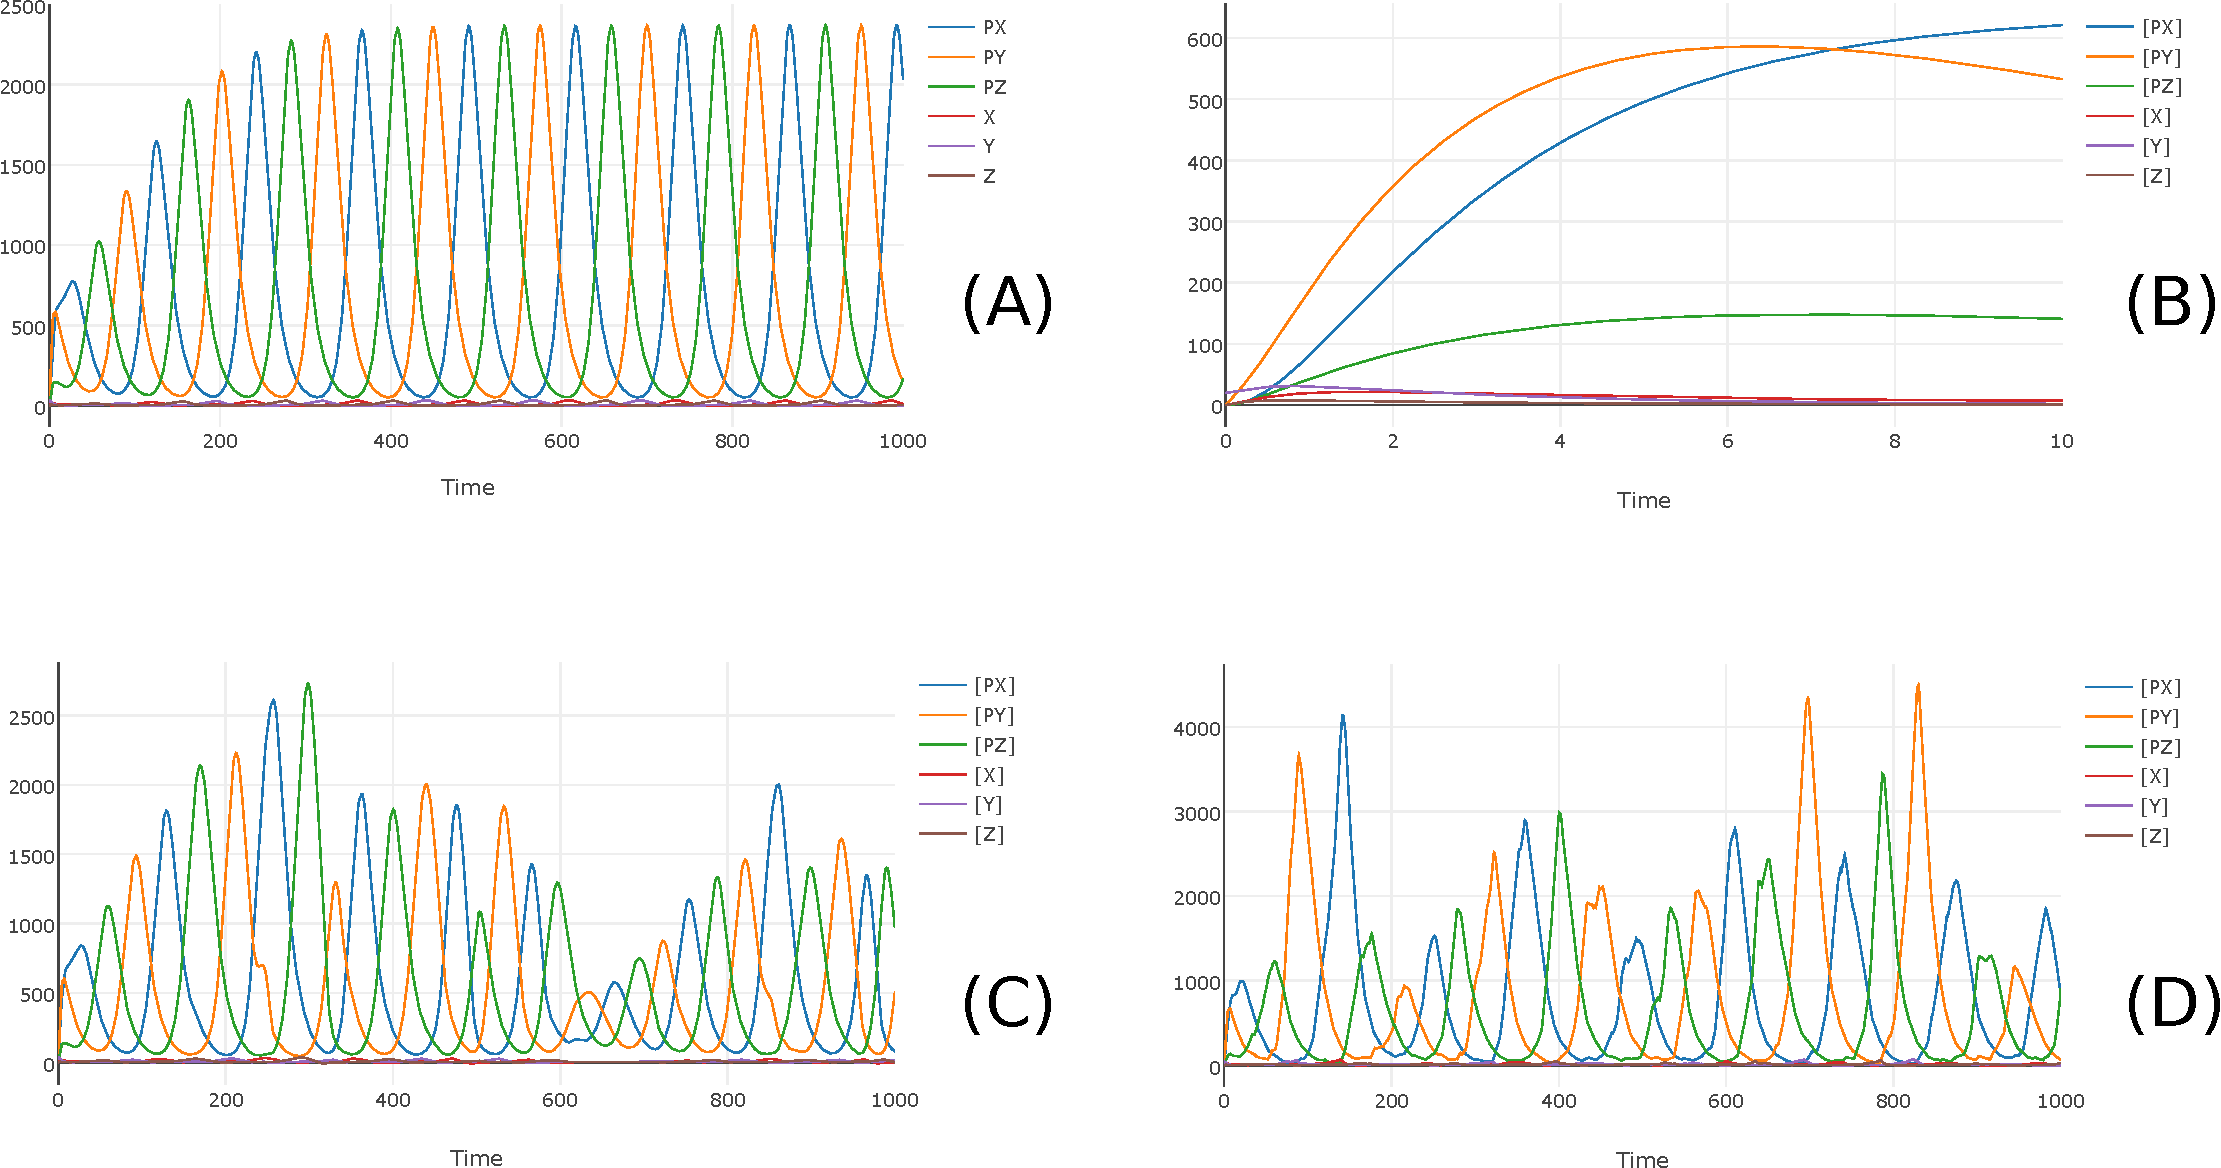
\includegraphics[width=\textwidth]{elowitz-simulations.pdf}
%   \caption{ Common mistakes in simulating a SBML model. This figure contains four different simulations of the same SBML model: the repressilator circuit \cite{elowitz2000synthetic} downloaded from the BioModels database (BIOMD0000000012). (A) shows the correct simulation with the intended timescale. (B) uses a timescale which is too short to reveal the oscillatory dynamics produced by the model. (C) uses softer tolerance values for the ODE integrator, causing an inaccurate solution. Most SBML simulators, including our software, use very stringent default tolerances in order to faithfully simulate even very sensitive models. However, reducing the stringency yields increased simulation performance, so tolerances should ideally be set on a per--model basis. Finally, (D) uses a stochastic solver based on the Gillespie method \cite{gillespie1977exact}, an easy mistake since SBML does not specify the intended solver. These mistakes can be avoided by providing a simulation experiment description in SED-ML specifying duration, time points, tolerance parameters, and simulation algorithm for the simulation. }
%   \label{fig:mistakes}
% \end{figure}

% \begin{figure}
%   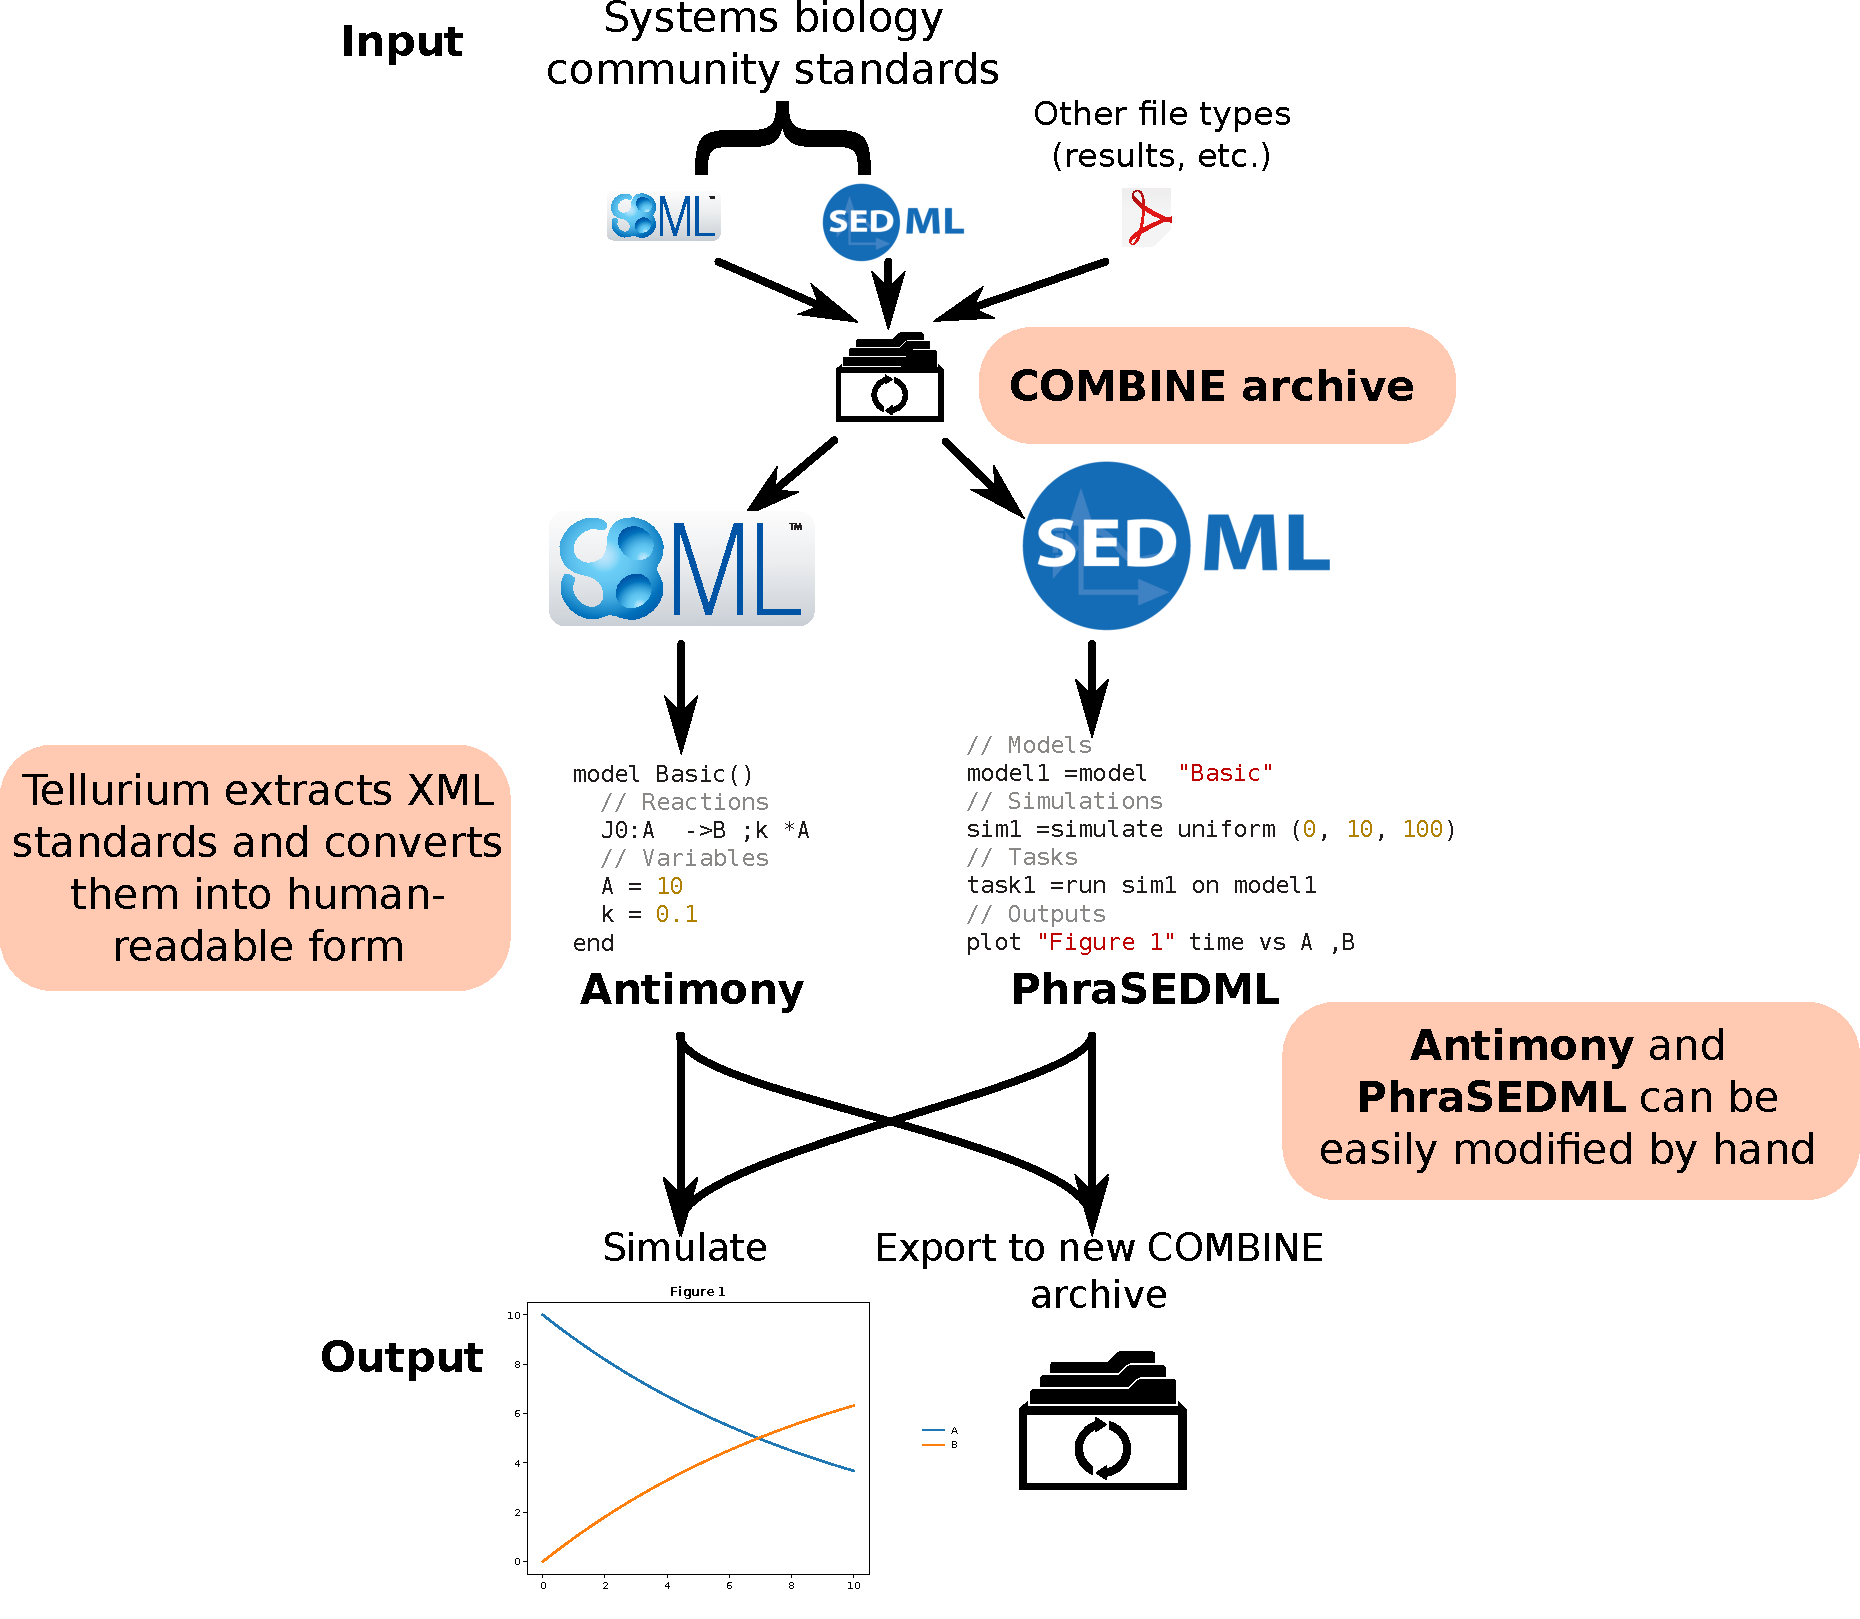
\includegraphics[width=0.75\textwidth]{fig-workflow.pdf}
%   \caption{A work-flow diagram for using Tellurium's reproducibility features. A COMBINE archive can contain standard encodings describing a model (encoded in SBML) and simulation (encoded in SED--ML). Tellurium converts these respective standard encodings into a human--readable form (Antimony \cite{smith2009antimony} and PhraSEDML \cite{choi2016phrased}) which are then used to run simulations and produce plots and reports. Any modifications made to the human--readable representations can be converted back to a COMBINE archive and re--exported.}
%   \label{fig:workflow}
% \end{figure}

% \begin{figure}
%   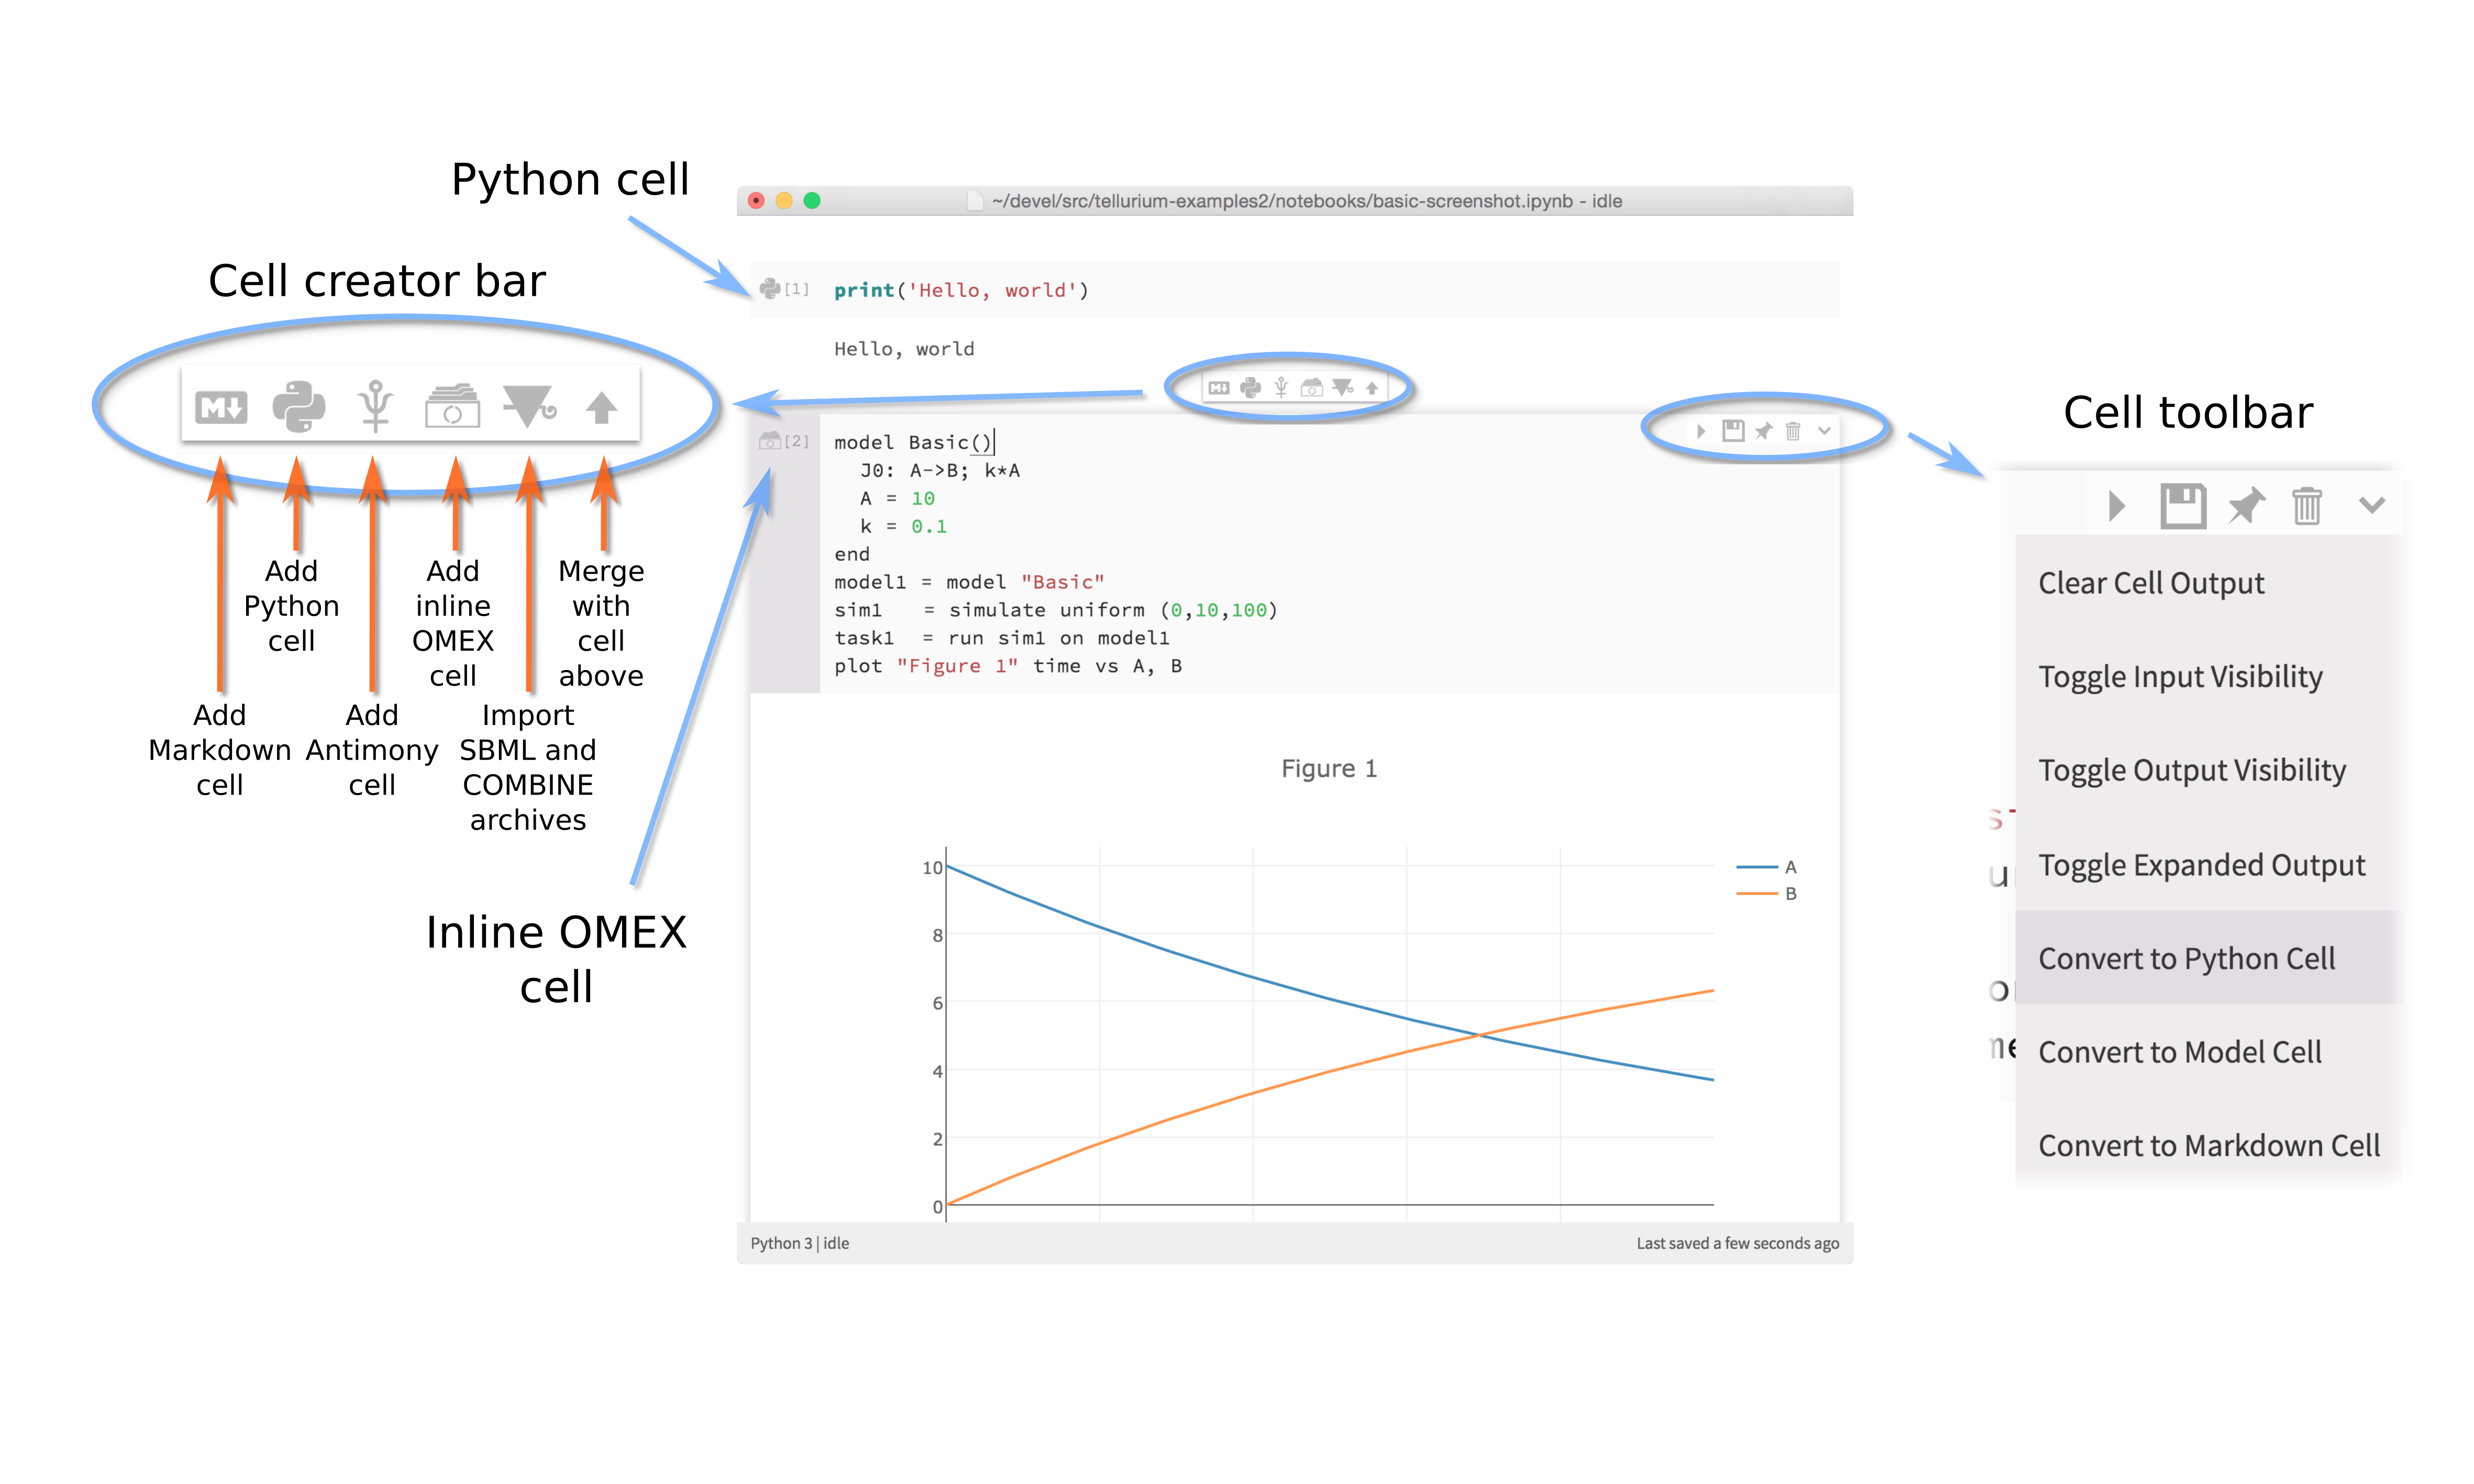
\includegraphics[width=\textwidth]{fig-interface.png}
%   \caption{The Tellurium notebook user interface, based on the \textit{nteract} app. Tellurium can also be installed as a collection of Python packages, in order to allow automated scripting or integration into a preexisting software environment. However, the notebook user interface provides additional usability features such as importing (by clicking the Tellurium icon followed by ``Import COMBINE archive'' or dropping the archive on the app) and exporting (by clicking the diskette icon in the cell toolbar) COMBINE archives and SBML files without prior knowledge of Tellurium's Python API, which eases the barrier to adoption. }
%   \label{fig:interface}
% \end{figure}

Tellurium supports embedding human--readable representations of SBML \cite{smith2009antimony} and SED--ML \cite{choi2016phrased} directly in cells. These cells can be exported as COMBINE archives which are readable by other tools. We refer to this human--readable representation as \textit{inline OMEX} (after Open Modeling and EXchange, the encoding standard used by COMBINE archives).
Inline OMEX cells operate in much the same way as code cells, i.e. they have syntax highlighting and are executable. Executing an inline OMEX cell runs all SED--ML simulations in the cell, producing any plots or reports declared in the SED--ML. A major advantage of this approach is that it offers a means of authoring transparent, exchangeable modeling studies without requiring technical knowledge of standards.


% what is it that we need in the tool requirements to work with standards. There has to be a way of representing stds in hr form. 2. take standard and translate into implementation. 3. generate specifications from implementation and repackage so others can use

% discuss what Tellurium provides: literate programming for transparency and COMBINE archive support for exchangeability

\section*{Results}

We demonstrate the benefits for reproducibility provided by Tellurium Notebook in a series of case studies. In the first case study, we explore the impact of variations in the value of a parameter in a model of yeast. Such explorations are frequently done to determine if a model is applicable to conditions beyond those in the original model, an important consideration for testing model validity. The second case study evaluates if a model implementation produces results that are comparable to those in the original study via a series of tests which cover important dynamical properties of the model.

\subsection*{Case Study 1: Assessing Previously Unexplored Model Parameters}

In order to meet our requirements for reproducibility, it is not sufficient to simply recreate a simulation. Rigorous reproducibility requires the ability to reuse, expand, and test existing models under a variety of circumstances. This first case study shows how Tellurium facilitates conducting new experiments with an existing model, including the packaging of the model and the experiments as a COMBINE archive. The study is based on a model of autonomous metabolic oscillations in yeast and associated numerical studies \cite{wolf2001mathematical}. The model has a cooperativity parameter $m$ for which no specific justification is provided. We explore a range of values of $m$ to understand how this parameter influences the dynamics in the model.

When grown in continuous culture, yeast exhibit oscillations that can be maintained for months and can cause the temporal separation of many cellular functions in a synchronized way \cite{murray2007regulation}. This type of dynamics belongs to a broader class of coupled oscillators that are thought to be highly important in the organization of circadian rhythms and play a role in the regulation of diurnal physiological activity in various species \cite{winfree1967biological,dodd2005plant}.
Wolf, et al. \cite{wolf2001mathematical} developed a model that uses metabolic coupling mediated in part by the $H_2 S$ pathway, one of the known contributors to respiratory oscillations in yeast \cite{murray2007regulation}, to explain experimentally observed synchronized oscillations in yeast cultures.

The model contains 21 reactions and is available via the BioModels repository as \texttt{BIOMD0000000090} \cite{wolfbiomod}. The reaction \texttt{v11a} is a key part of the $H_2S$ pathway. As shown in Fig  \ref{fig:comparison}, standard--encoded SBML for this reaction is difficult to decipher, much less comprehend. As with other authoring tools, Tellurium provides a concise, human--readable abstraction of this encoding. However, unlike other tools, this abstraction covers the entire SBML model and even covers entire COMBINE archives as we show shortly. We focus on the human readable representation of the reaction \texttt{v11a}, including the reaction kinetics using the Hill coefficient $m$.

\begin{figure}
  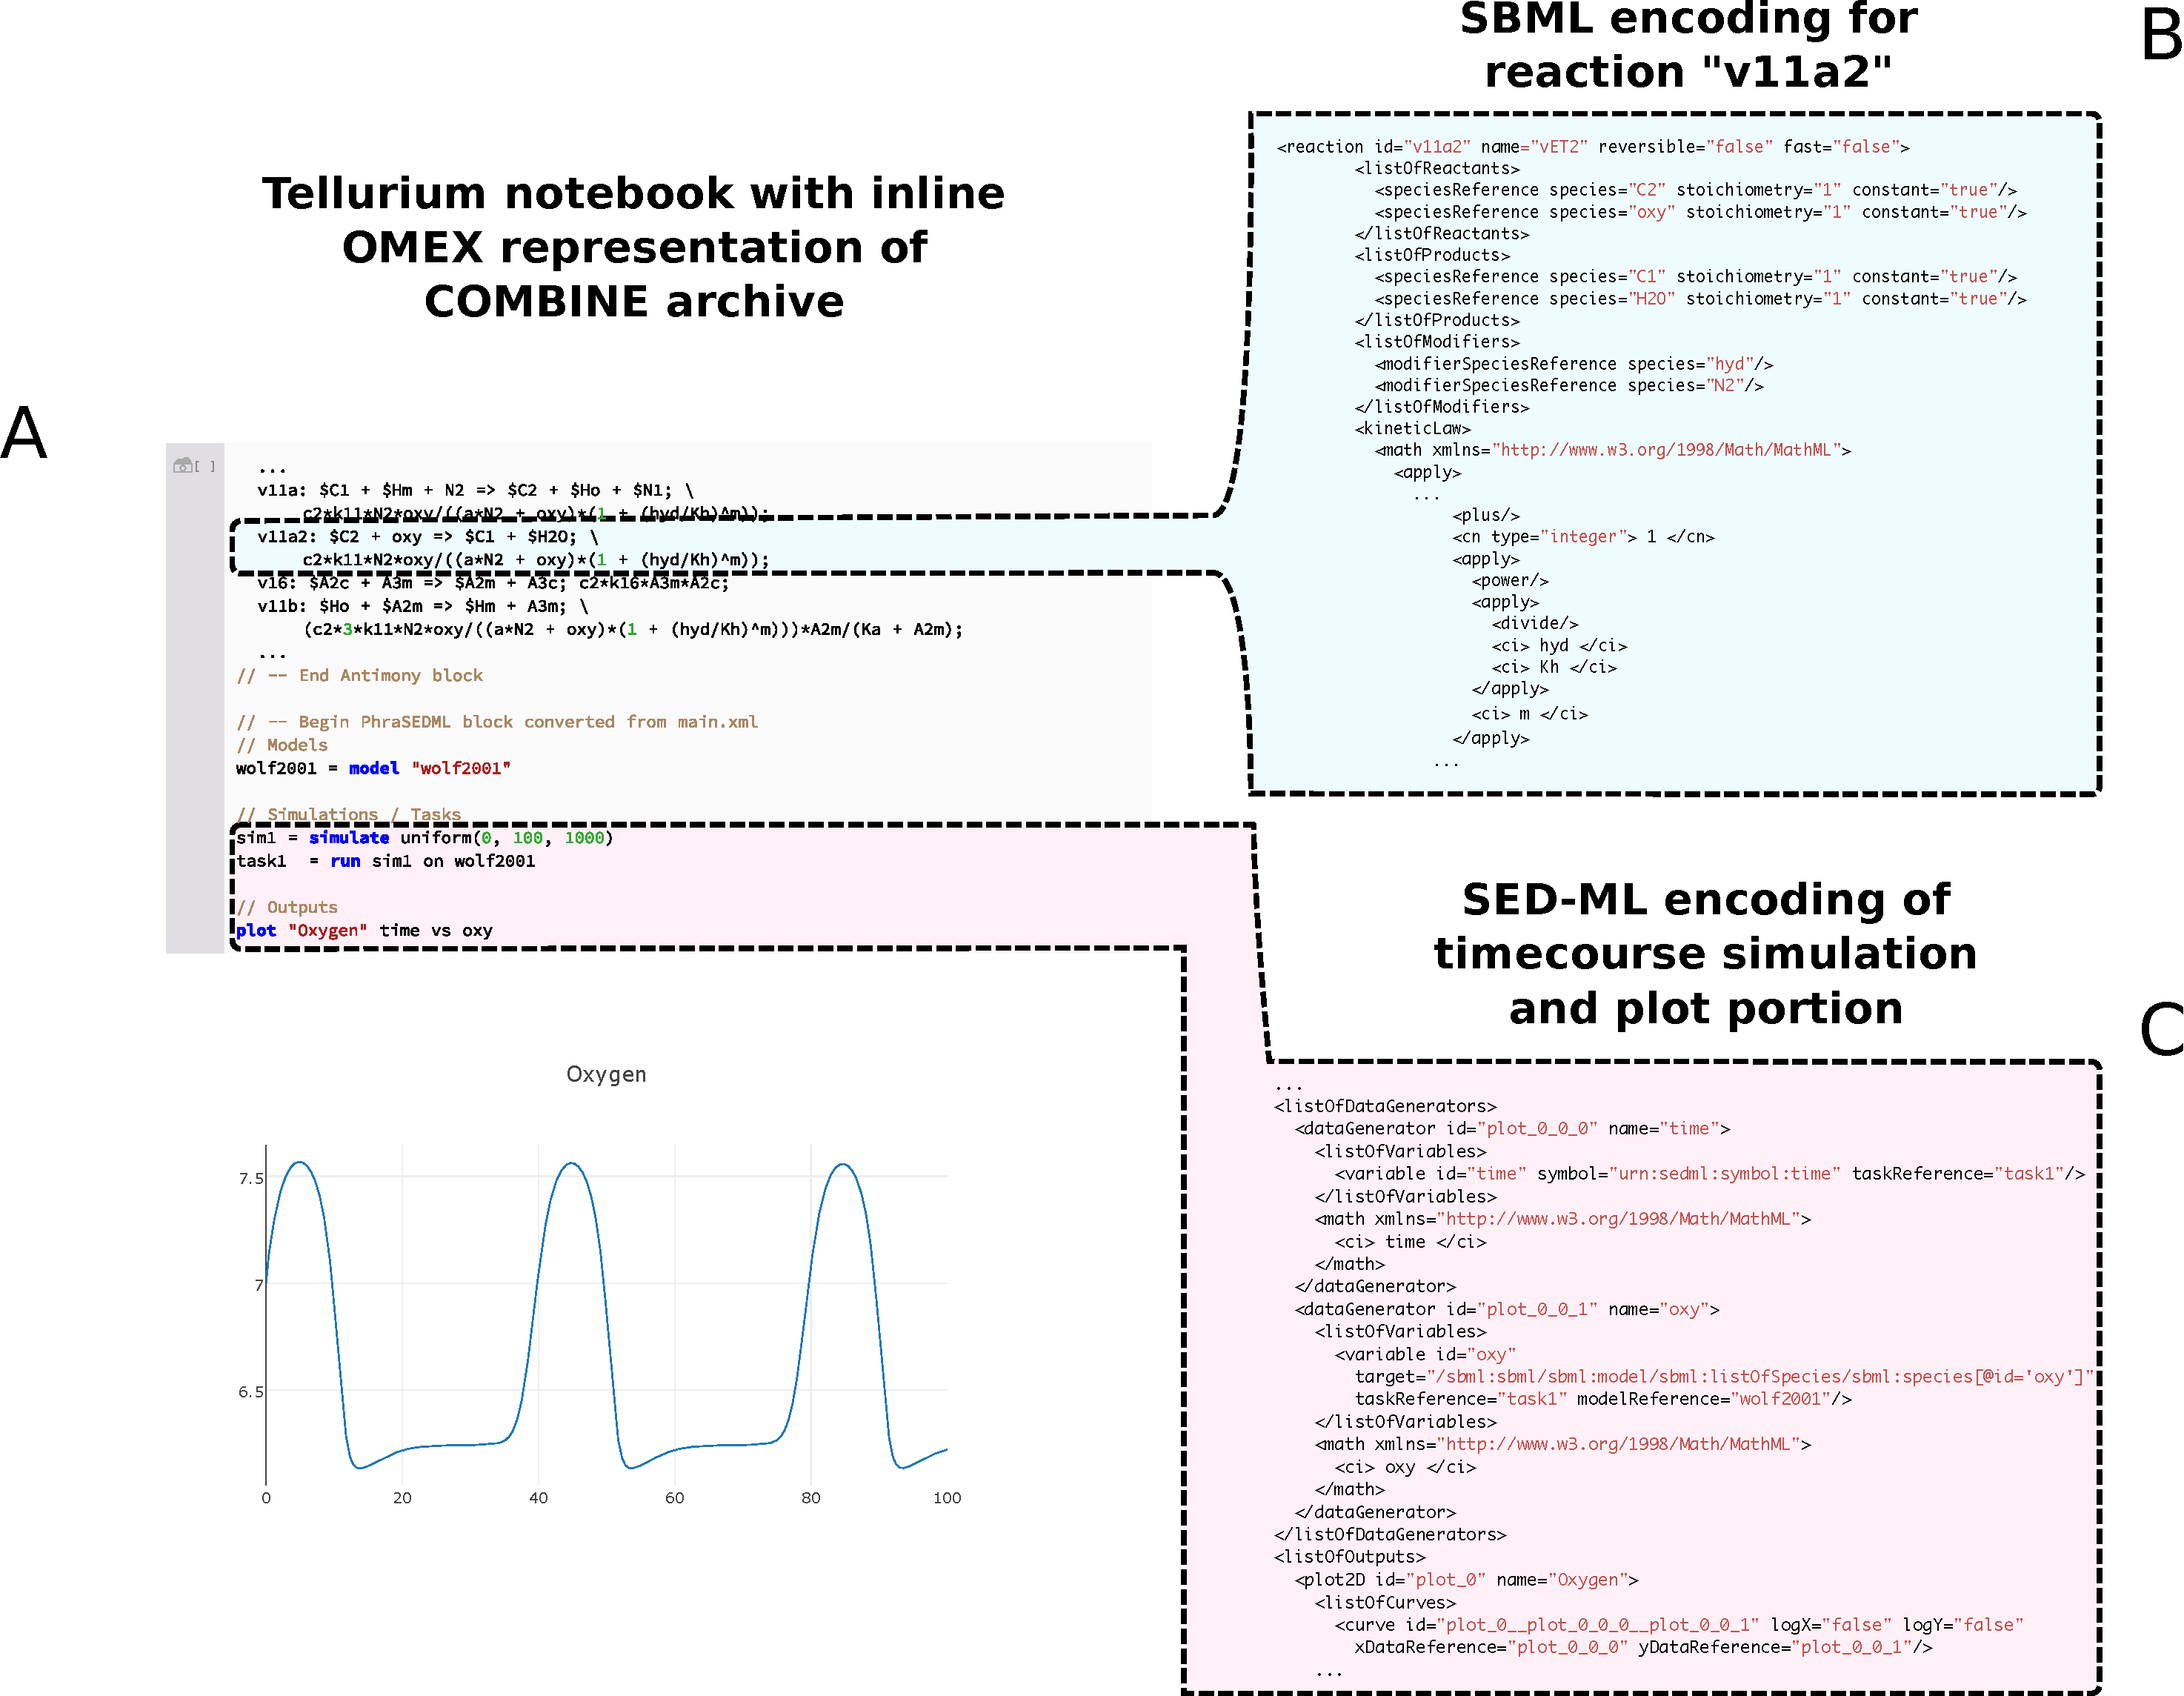
\includegraphics[width=\textwidth]{fig-comparison2.pdf}
  \caption{A comparison of Tellurium's human--readable representation of a COMBINE archive shown in a Tellurium notebook (A) and excerpts from the equivalent SBML (B) and SED--ML (C) encodings. Tellurium's in-line OMEX format contains human--readable representations of both SBML and SED--ML (A). (B) contains the SBML encoding for a single reaction. The single--line human--readable form of this reaction is highlighted in part (A) for comparison. Using the SBML encoding, it is difficult to modify the reaction stoichiometry or kinetic law, whereas this task is easy in Tellurium. This example makes use of a model of respiratory oscillations in yeast \cite{wolf2001mathematical} and is available as a COMBINE archive \cite{wolfoxy}. }
  \label{fig:comparison}
\end{figure}

Clearly, readability is essential for model transparency. However, readability is essential for model reuse as well. To demonstrate this, we convert this SBML--only model into a COMBINE archive containing both SBML portions describing the model and SED--ML portions describing the simulation.  Then, we show how Tellurium's human--readable format permits easy modification of the study contained in the COMBINE archive.

% We will begin by downloading this model and importing it into Tellurium by clicking on the \texttt{File} menu and selecting \texttt{Import SBML...} from the Tellurium notebook app. Tellurium transparently converts SBML into a human--readable form and creates a new cell displaying the model. In order to add a SED--ML simulation specification to the model, let us convert the SBML cell into an in-line OMEX cell by selecting \textit{Convert to OMEX cell} from the cell toolbar dropdown. Then, we can add four lines describing the human--readable SED--ML as shown in Fig \ref{fig:comparison}. For comparison, Fig \ref{fig:comparison} also shows the equivalent SBML (for only a single reaction) and SED--ML describing this model and simulation. Pressing shift--enter to execute the in-line OMEX cell causes Tellurium to transparently convert the human--readable format into the corresponding SBML and SED--ML and run all simulations described in the SED--ML. Clicking on the diskette icon in the cell toolbar exports the contents of the cell to a COMBINE archive containing SBML and SED--ML, which can be imported by other tools such as the SED--ML Web Tools \cite{bergmann2017sed}.

% The human--readable SBML shows that the model contains three reactions (\texttt{v11a}, \texttt{v11a2}, and \texttt{v11b}) which make use of the Hill coefficient $m = 4$. The original authors do not provide any rationale for this choice of Hill coefficient \cite{wolf2001mathematical}, so we demonstrate Tellurium's editing capabilities by exploring the effect of different values of $m$ on the model's timecourse dynamics.

In order to create a SED--ML specification for this model, we need to define four steps in the workflow, which correspond to distinct elements in SED--ML: (1) model definition, (2) simulation, (3) task specification, and (4) output generation. For (1), models can be defined in Tellurium's human--readable format by referencing SBML or CellML files in the same COMBINE archive, with the option of including parameter replacements. For (2), SED--ML simulations can be either timecourse simulations or steady state computation, and can reference a specific algorithm (e.g. LSODA), or a generic implementation using the KiSAO ontology \cite{courtot2011controlled}. Tellurium uses predefined keywords such as \texttt{lsoda} (an ODE solver implementation \cite{petzold1997lsoda}) to refer to popular implementations. In SED--ML, simulations are specified independently from models. This allows model and simulation elements to be reused in different combinations. For (3), SED--ML uses task elements to describe these combinations. Finally, the output elements of (4) can be plots or reports and allow users to access the output of tasks. Tellurium's human--readable format allows defining a SED--ML model by instantiating the same SBML model with different parameter values ($m$ in this example) using the syntax:
\newline
\newline
\texttt{mymodel = model "wolf2001" with \textbf{param1}=\textbf{value2}, \textbf{param2}=\textbf{value2} ...}
\newline
\newline
with the param/value pairs being replaced by the corresponding parameter ids and values respectively. We use this syntax to instantiate five copies of the model and explore the values $m=1,2,4,8,16$. Since we do not know \textit{a priori} if the value of $m$ affects the timescale of the dynamics, we also create two simulations using different durations. Finally, we create a task for each model/simulation combo and plot the results on their respective timescales. Fig \ref{fig:hill} shows that the value of $m$ drastically affects the dynamical behavior of the system, abolishing the periodicity of the oscillations at $m=8$ and ceasing them entirely at $m=16$. Smaller values of $m$ also affect the phase and amplitude of the oscillations.

\begin{figure}
  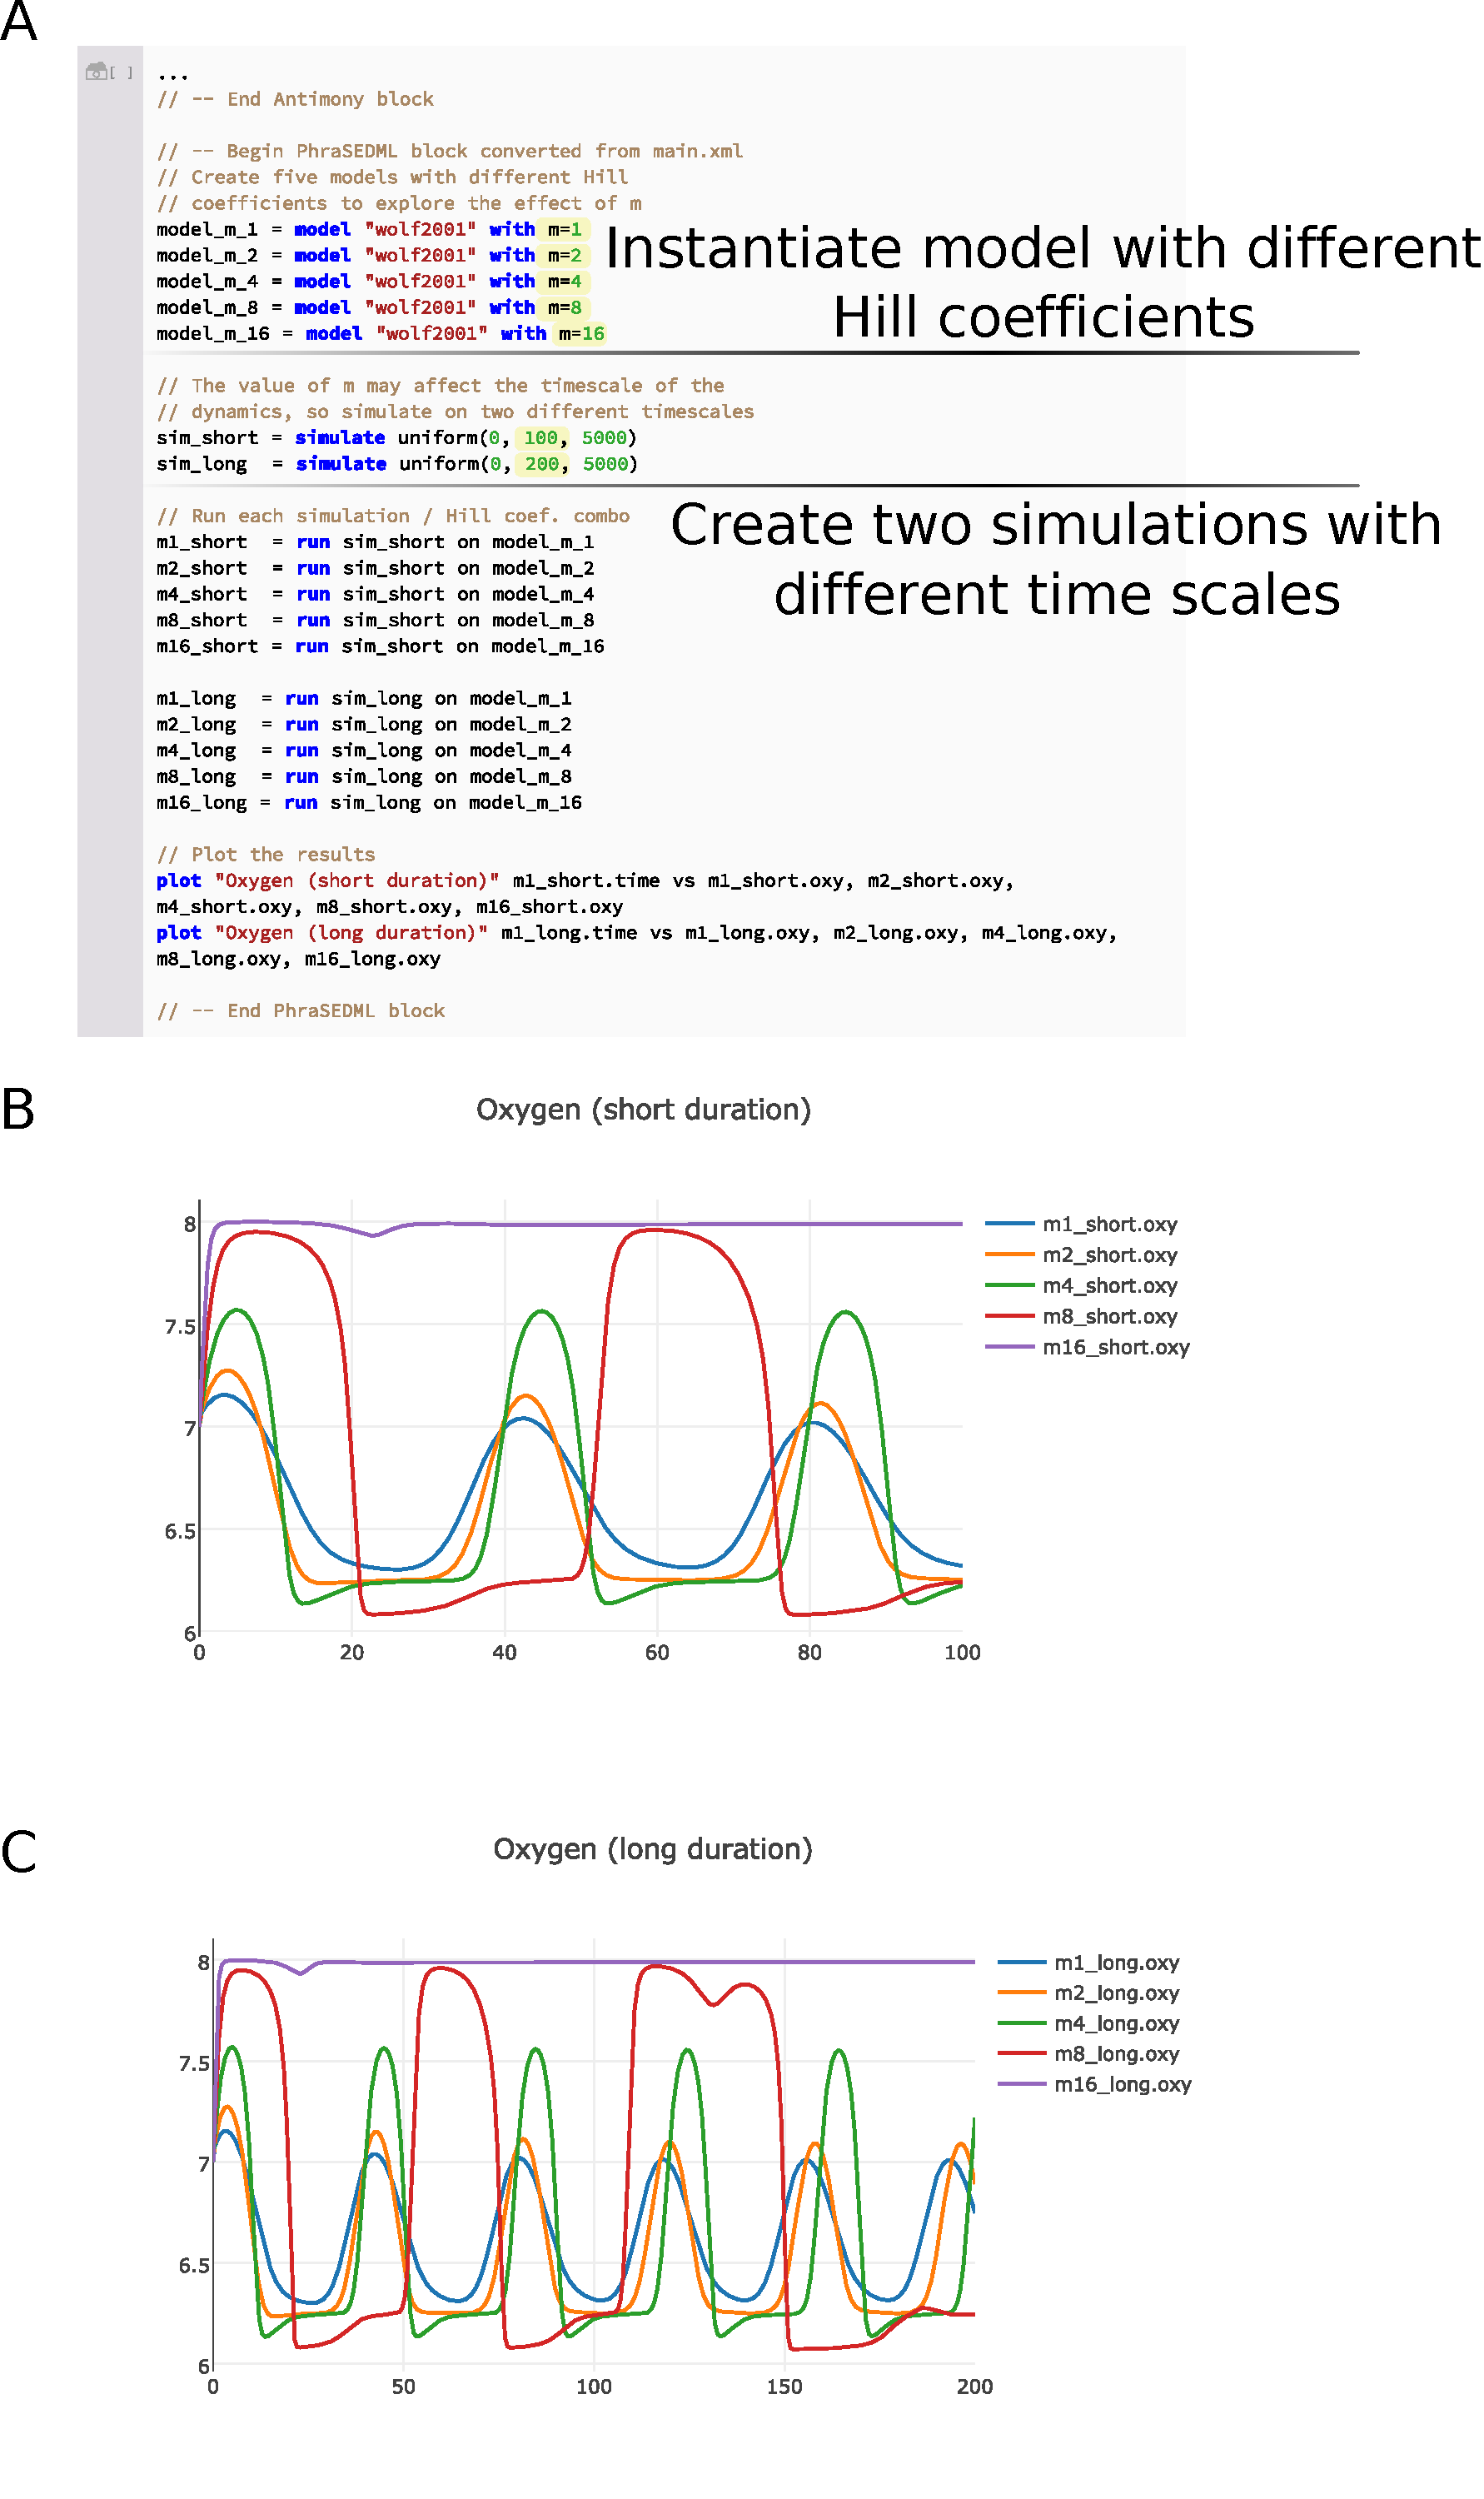
\includegraphics[width=0.85\textwidth]{fig-hill2.pdf}
  \caption{An example of using Tellurium to edit the respiratory oscillations model introduced in Fig \ref{fig:comparison}. To investigate the effect of the Hill coefficient $m$, we used Tellurium's human--readable representation of SED--ML to create five instantiations of the model using values of 1, 2, 4, 8, and 16 for $m$ (A). We then simulated each of these instantiations on two different timescales and plotted the respective results for short (B) and long (C) simulations. Tellurium's COMBINE archive support allows this model and simulation to be exported to other tools, as shown in Fig \ref{fig:swt} }
  \label{fig:hill}
\end{figure}

%This parameter exploration indicates that the cooperativity parameter $m$ is highly important for the dynamics of the model. While this conclusion does not determine whether the parameter is closely tied to biological constraints, it does establish the necessity of the original value for accurately reproducing the dynamics of the system. Tellurium allows users to easily create model variants to uncover important relationships such as these in an exchangeable workflow. Furthermore

This case study shows that Tellurium provides an efficient means of converting SBML models into exchangeable COMBINE archives containing simulation components. Furthermore, COMBINE archives can contain important dynamical information about the model, such as the influence of the parameter $m$ that we explored in this study. In order to demonstrate exchangeability of this study, we have exported it to the SED-ML Web Tools \cite{bergmann2017sed} (Fig \ref{fig:swt}) and iBioSim \cite{myers2009ibiosim} (Fig \ref{fig:ibiosim}).

\subsection*{Case Study 2: Reproducibility Through In--depth Variational Studies}

Reproducibility requires that a model implementation produces results consistent with the original study, especially if a different authoring tool is used. In order to provide criteria for judging whether a model reproduction is consistent with the original, a set of testing criteria are required, similar to the concept of unit testing in software.
However, researchers seldom perform extensive checks on the dynamics of models before using them. This is due in part to the lack of tool support for easily modifying and producing variants of models and simulations encoded in exchangeable formats.
Tellurium's authoring features enable modelers to encode dynamical unit tests in COMBINE archives, thereby providing a way to verify that a model has been correctly reproduced.

For this case study, we reproduce a highly--detailed model of syncytial nuclear divisions in the \textit{Drosophila} embryo \cite{calzone2007dynamical} through testing the model's dynamics under different conditions.
%The authors of this model conducted extensive variational studies using different parameter combinations. This large set of variants allows us to perform in--depth validation of the dynamical behavior of the model.
In many insect species, the embryo enters a period of rapid mitotic division without cytokinesis \cite{gilbertDevBiol} immediately following fertilization. In \textit{Drosophila}, 13 of these divisions occur within 3 hours of fertilization \cite{calzone2007dynamical}. These divisions are regulated by metaphase promoting factor (MPF), a complex between cyclin (specifically the cyclin CycB in this model) and cyclin--dependent kinases (Cdk). CycB subunits tend to be the limiting factor in complex formation, and are thought to regulate mitotic division. CycB availability is controlled by the anaphase promoting complex (APC), which targets CycB for degradation. However, in \textit{Drosophila}, the levels of CycB appear to remain high during the first 8 mitotic divisions \cite{edgar1994distinct}. This observation can be reconciled with known mechanisms by assuming that CycB degradation only occurs in the vicinity of the mitotic spindle \cite{calzone2007dynamical,huang2002dynamic,raff2002roles}, despite the absence of a nuclear envelope during the mitotic divisions. To account for this hypothetical local degradation of CycB, the model artificially separates the cytoplasm into two ``compartments,'' with a cytoplasmic compartment representing the cell and a nuclear compartment representing the volume in the vicinity of the mitotic spindle.%

As a starting point, we use the COMBINE archive encoding of this model by Scharm and Tour\`{e} \cite{scharmShowcase}. This archive contains SBML derived from biomodel \texttt{BIOMD0000000144} \footnote{https://www.ebi.ac.uk/biomodels-main/BIOMD0000000144}, which is intended to reproduce Fig 1 of \cite{calzone2007dynamical}. However, the archive does not contain more extensive tests of the model's dynamics, such as whether the model can be used to reproduce several other simulations described  in the paper. The initial variant encoded by the COMBINE archive and shown in Fig \ref{fig:calzone}B and C is based on a model with a constant level of the phosphatase String, whereas in reality String levels change over the course of the mitotic cycles. String regulates MPF via a positive feedback loop, and has been shown to peak at the seventh or eighth cycle of the mitotic divisions \cite{calzone2007dynamical}. To account for this, Calzone et al. \cite{calzone2007dynamical} posited that String mRNA is degraded by a hypothetical factor ``X,'' causing the synthesis rate of String to drop over time.
Therefore, we have modified the SED--ML of the original COMBINE archive \cite{scharmShowcase} as follows to include the synthesis and degradation of String. With these modifications, we are able to reproduce Fig 3 of \cite{calzone2007dynamical}:

\begin{figure}
  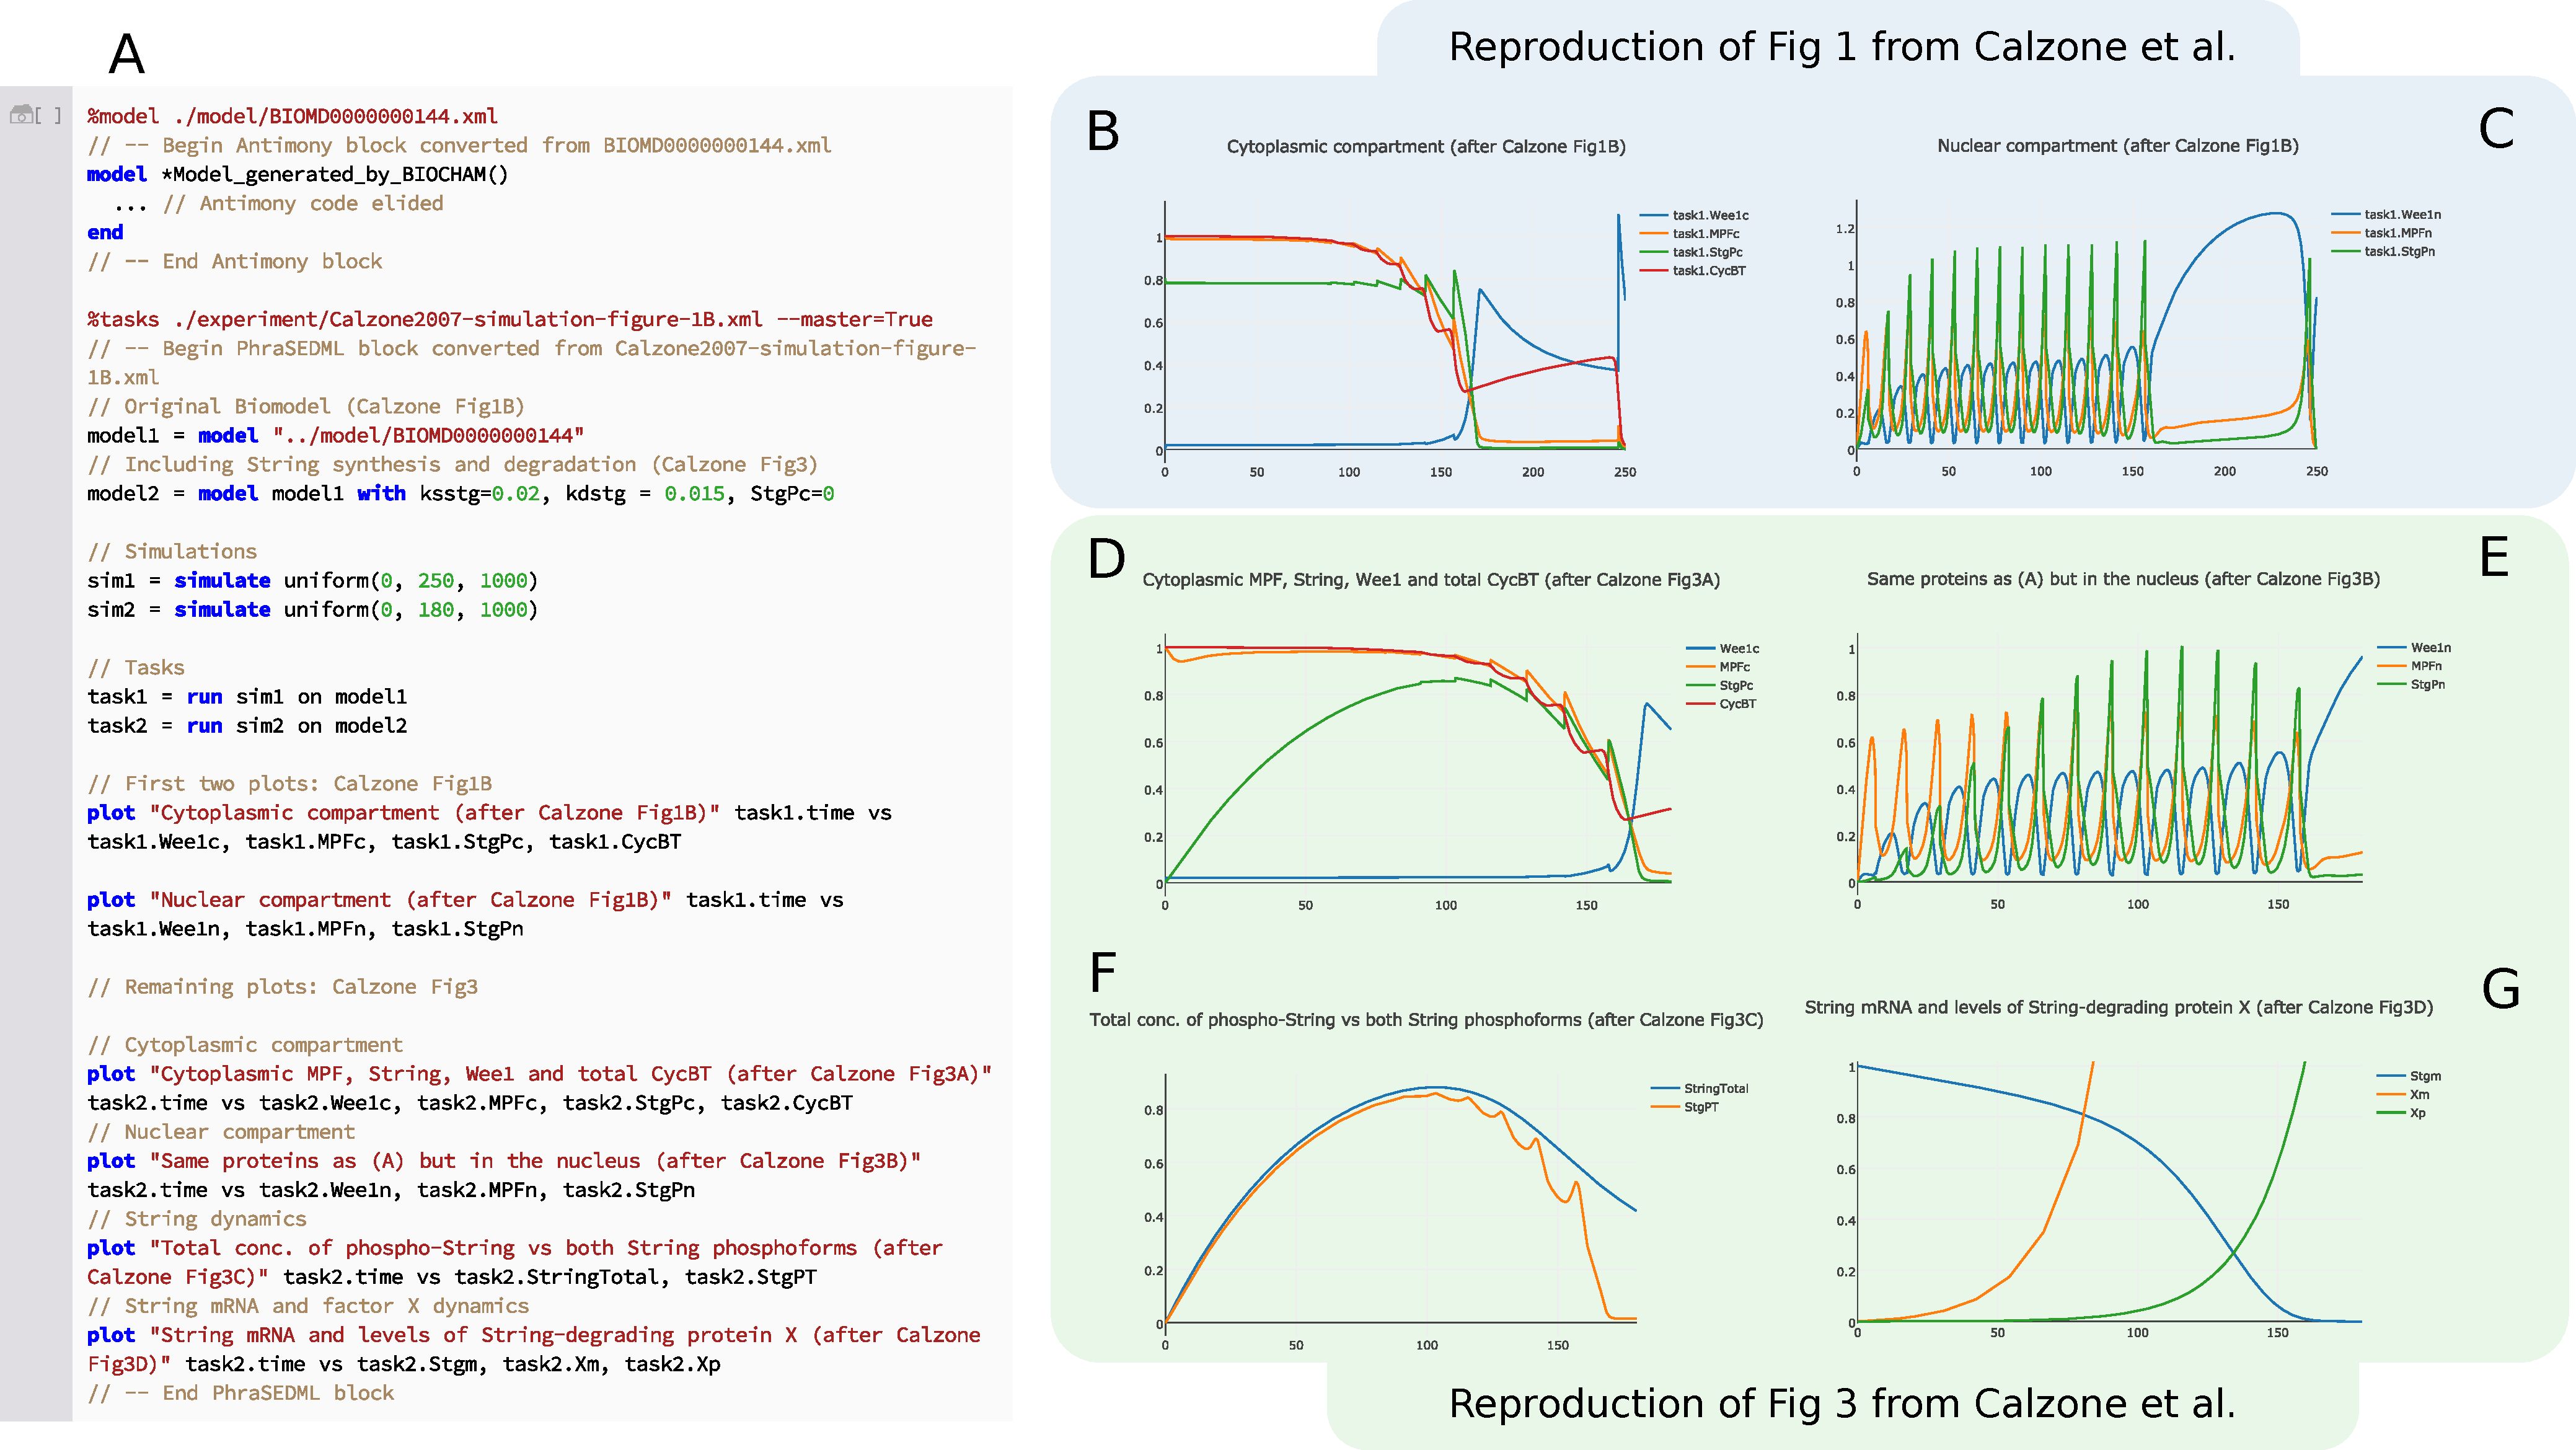
\includegraphics[width=1.0\textwidth]{fig-calzone.pdf}
  \caption{Using Tellurium to reproduce model variants in \cite{calzone2007dynamical} and repackage as a COMBINE archive. To demonstrate the use of COMBINE archives for encoding model variants, we began with a COMBINE archive describing a single variant of this model without String synthesis or degradation \cite{scharmShowcase}, which reproduces Fig 1B of \cite{calzone2007dynamical} (plots B and C here). We then used Tellurium to add a variant describing String degradation, which reproduces Fig 3 of \cite{calzone2007dynamical} (plots D through G here). Plots B and D show the cytoplasmic compartment of the model. Plots C and E show the nuclear compartment (defined as the spatial region around the mitotic spindle). Plot F shows the levels of total String and its phosphorylated state. Plot G shows the level of String mRNA and protein factor X, which degrades String mRNA. The y--axis scale on plot G was manually adjusted to show the mRNA dynamics. The COMBINE archive for this example is available online \cite{calzone-fig1-fig3}. The subplots in this figure intentionally have different durations, after Calzone et al \cite{calzone2007dynamical}. The model in \cite{calzone2007dynamical} was authored using BIOCHAM \cite{calzone2006biocham}. }
  \label{fig:calzone}
\end{figure}

\begin{itemize}
\item Enable synthesis and degradation of String by setting the parameters \texttt{ksstg=0.02} and \texttt{kdstg=0.015} respectively.
\item Set the initial concentration of total String to zero by setting \texttt{StgPc=0}.
\item Compute the total amount of unphosphorylated String by adding the rule \newline \texttt{StgT := (1 - N*E\_1)*Stgc + N*E\_1*Stgn}.
\item Compute the total amount of String in the cell by adding the rule \newline \texttt{StringTotal := StgPT + StgT}.
\end{itemize}

Tellurium makes it easy to encode both the original variant, without String synthesis and degradation, and the variant including these terms, in a COMBINE archive \cite{calzone-fig1-fig3}. Fig \ref{fig:calzone} shows the results of executing this COMBINE archive in Tellurium. We have thus expanded the dynamical test cases for this model, as it now reproduces two simulations from two different variants described by the original authors (Fig 1 and 3 of \cite{calzone2007dynamical}), enabling better coverage of the model's dynamics.

In order to gain insight into the regulatory mechanism controlling the mitotic divisions, and understand the transitions that control the exact number of these divisions, Calzone et al. performed a one--parameter bifurcation analysis \cite{calzone2007dynamical}. Bifurcation analyses probes the number and position of steady states and other types of attractors as a function of a parameter. The oscillations shown in Fig \ref{fig:calzone} are the result of discrete division events, and the behavior shown does not represent a limit cycle. However, the model can be shown to exhibit limit cycle behavior by 1) removing all discrete events and 2) fixing the number of divisions by introducing the variable $C$ as a cycle counter. The number of nuclear compartments is then given by $N = 1.95^C$ (1.95 is a scaling factor described in \cite{calzone2007dynamical}). For a given cycle number $C$, MPF exhibits limit cycle oscillations, although the amplitude and period of these oscillations changes with the cycle number. At low cycle number, Calzone et al. observed that these oscillations were dominated by the negative feedback effect of cyclin degradation, whereas for large cycle number ($C \ge 12$), positive feedback via control of phosphorylated MPF by the kinase Wee and phosphatase String contributes to the oscillations.

SED--ML does not support bifurcation analysis, precluding us from reproducing that part of the study in an exchangeable format. However, it is still possible to test the change in regulatory shift from negative to positive feedback. Instead of a bifurcation diagram, we compare the limit cycle behavior of the original model to a model variant with reduced Wee and String activation and deactivation rates. This slows the timescale of the positive feedback component of the model. Fig \ref{fig:calzone-limit-cycles} compares the behavior of the original model at early and late cycle numbers with the variant containing attenuated positive feedback. Whereas the normal model exhibits stable limit cycle oscillations at both $C=1$ and $C=12$, the oscillations in the attenuated model are transient at late cycles ($C=12$) but not at early cycles ($C=1$). This observation suggests that String and Wee dynamics are indeed crucially important for late cycle oscillations, but not for early cycle oscillations, confirming the shift in regulatory mechanism. These simulation thus form a third set of unit tests for the model, encoded as a COMBINE archive \textbf{TODO: ADD ARCHIVE}.

\begin{figure}
  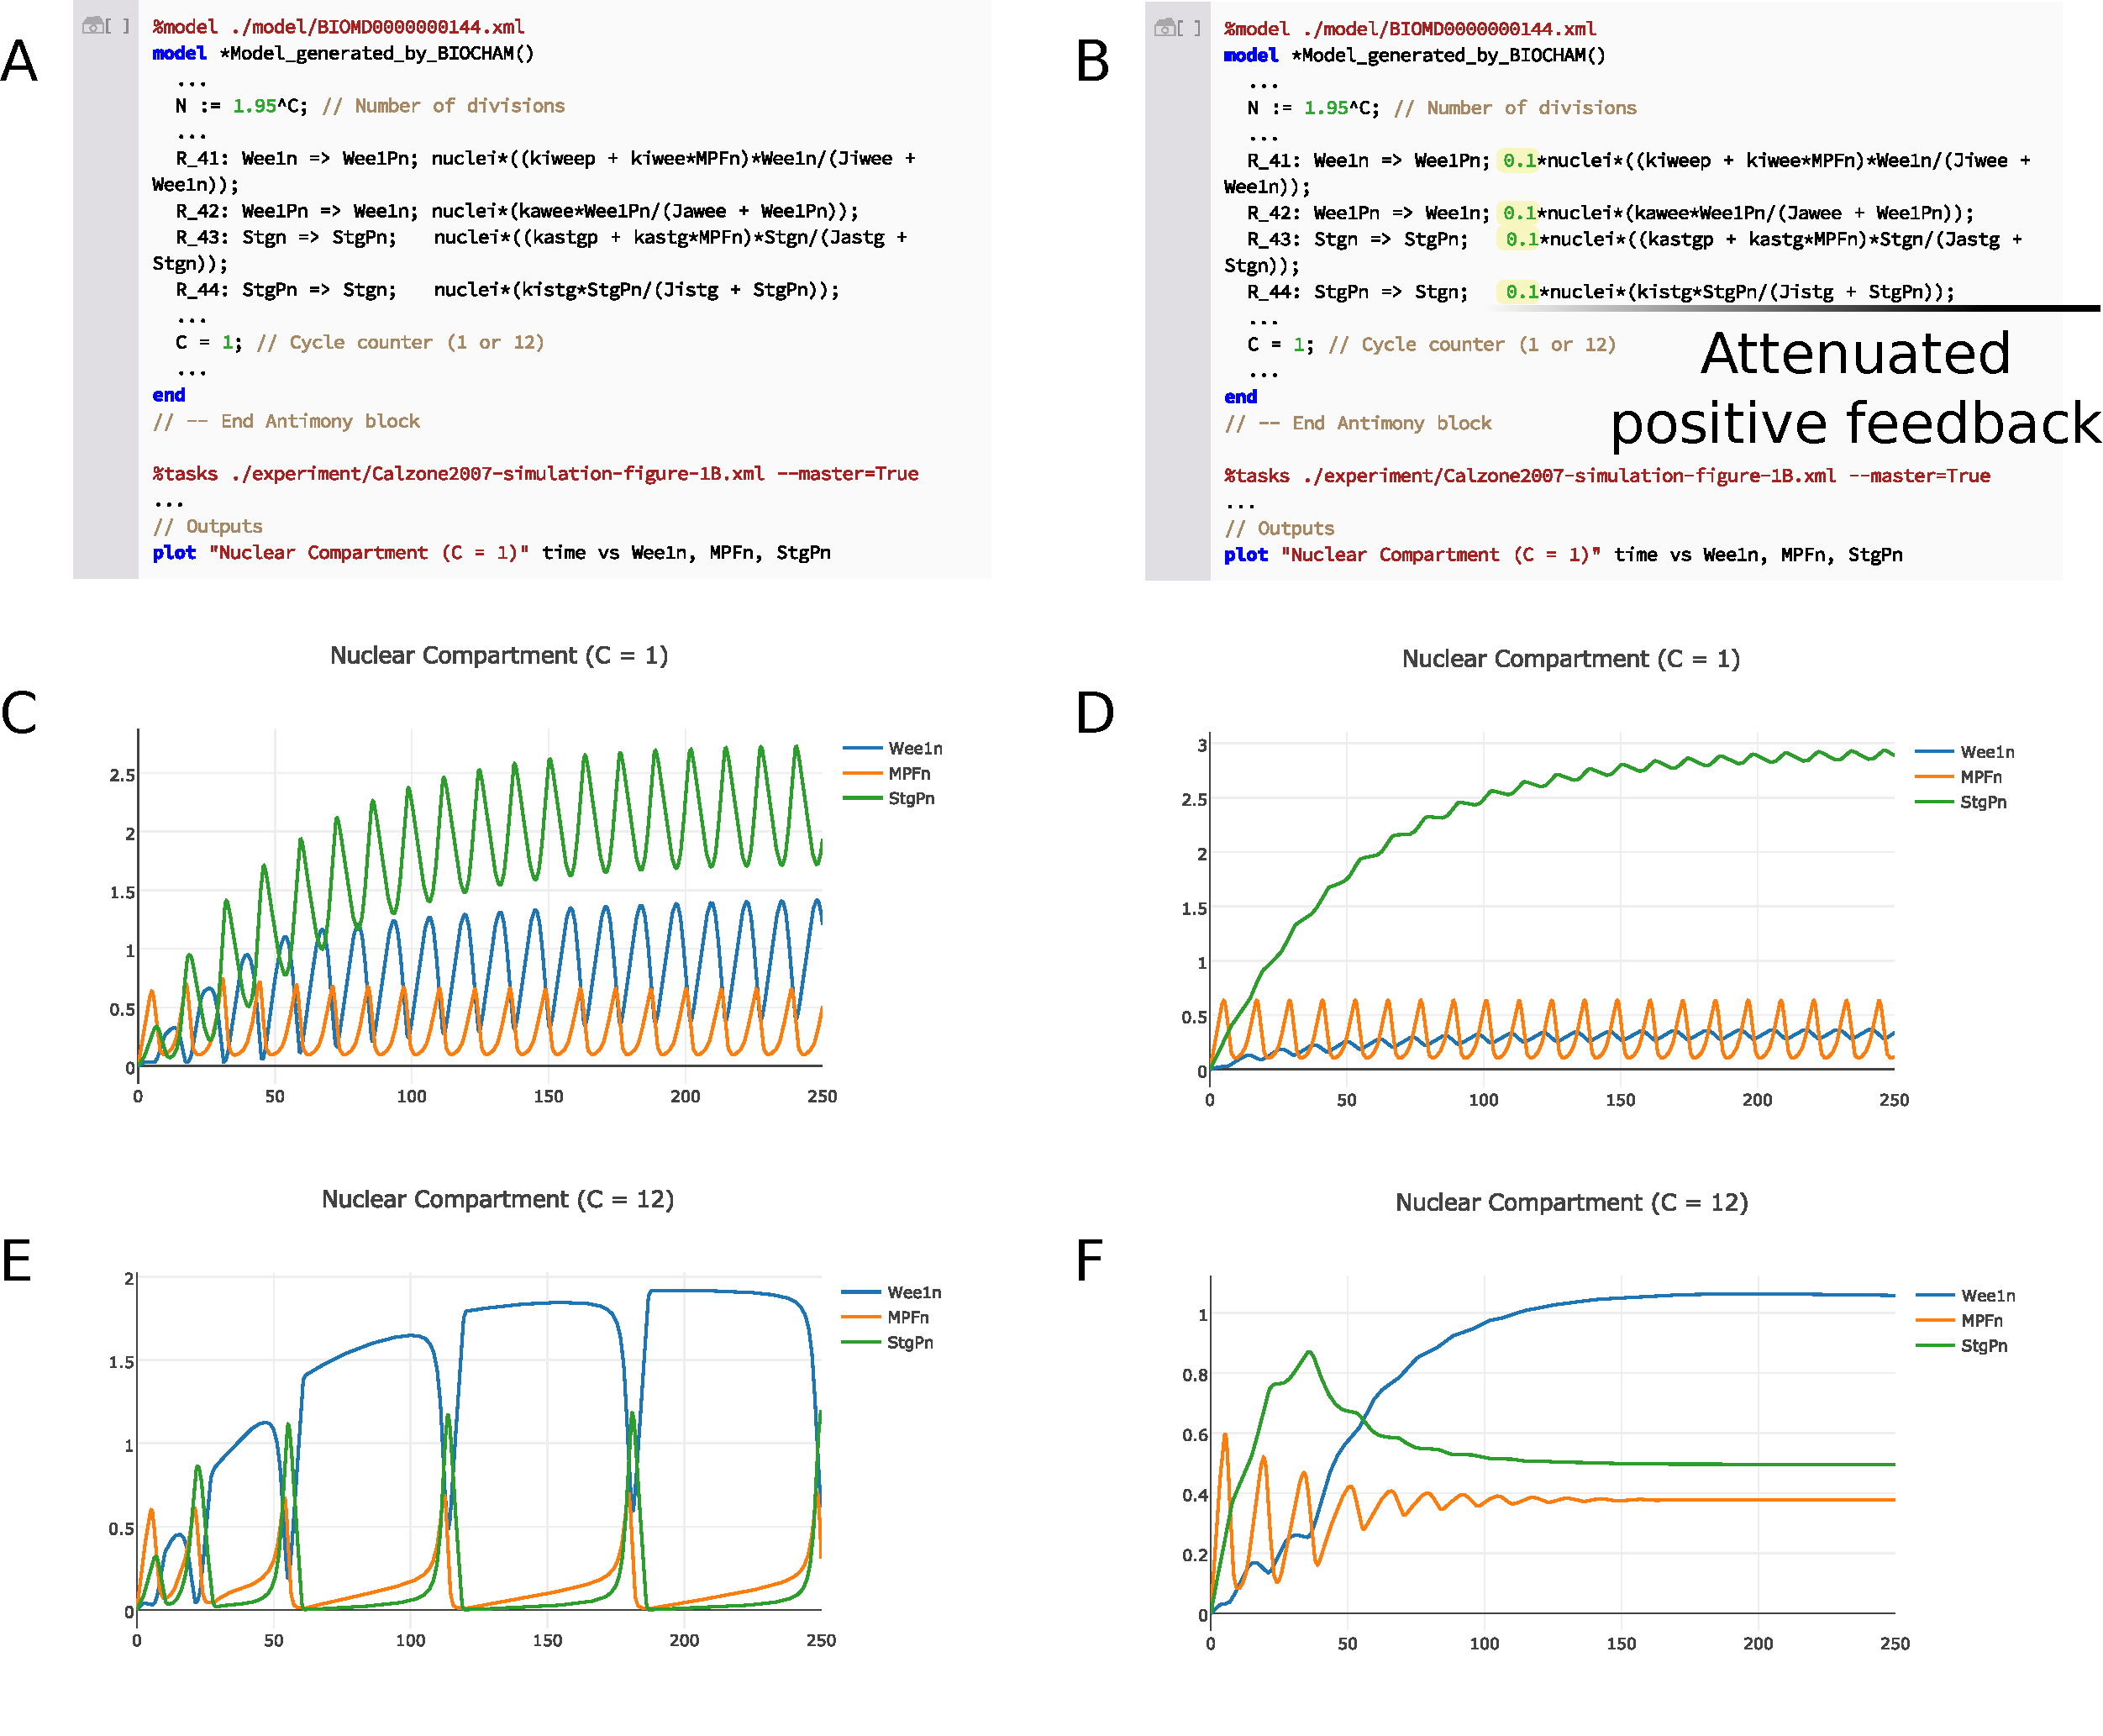
\includegraphics[width=1.0\textwidth]{calzone-limit-cycles.pdf}
  \caption{Testing the shift in regulatory mechanism of mitotic oscillations. To verify the observation \cite{calzone2007dynamical} that the number of mitotic divisions in the \textit{Drosophila} embryo is governed by a shift from negative to positive feedback, we first removed all discrete events and introduced the variable $C$ such that $N=1.95^C$. We then compared the limit cycles produced by this eventless model (left) with those produced by a variant with attenuated positive feedback from the regulators Wee and String (right). Attenuation was achieved by decreasing the rates of the phosphorylation and dephosphorylation of Wee and String. The original model exhibits stable limit cycle oscillations for both early cycles (C), which are putatively dominated by negative feedback, and late cycles (E), which are putatively dominated by positive feedback. The attenuated model only exhibits stable oscillations at early cycles (D), suggesting that positive feedback does indeed play a role in late cycle oscillations (F). This study is available as a COMBINE archive \cite{calzone-feedback-archive}. }
  \label{fig:calzone-limit-cycles}
\end{figure}

In summary, using Tellurium's editing capabilities, we have created an extensive set of unit tests for dynamical behavior this model, which we exported as a COMBINE archive and imported into another tool as shown in Fig \ref{fig:swt-calzone}. Creating these tests required a means of quickly editing and expanding upon both the SBML and SED--ML embedded in the COMBINE archive. Tellurium's notebook approach allows us to satisfy these requirements, and provides an integrated workflow for testing the dynamical behavior of the model.

\subsection*{Interoperability Concerns \& Test Cases}

In order to achieve the exchangeability requirement of reproducibility, broad standards compliance is necessary. A small number of test cases, such as the first two case studies, is not sufficient to ensure interoperability with other software.
%Due to the recent introduction of the COMBINE archive specification \cite{bergmann2014combine} and supporting libraries \cite{bergmann_frank_t_2016_154158}, many tools do not yet support the standard.
%Unfortunately, there are few examples of COMBINE archives.
During Tellurium's development, we gathered a number of COMBINE archive exemplars from the literature, other software tools, and our own archives. We have provided these archives as a resource to other developers by making it publicly available online. The test archives are structured to separate examples with advanced SED--ML features from those with basic SED--ML usage, enabling tool developers to implement incremental support for the standard. Table \ref{combine-archive-tests} lists all test archives and how to obtain them.

%These tests help ensure that is broadly standards compliant. The tests may also help others to implement support for COMBINE archives. Therefore, we have collected the extensive set of COMBINE archives used for our internal testing in a repository. This repository all case studies used in this manuscript. In order to aid other tools in implementing COMBINE archive support, the test suite contains archives ranging from basic examples to advanced usage of the SED--ML standard. The test suite a combination of cases generated by us and cases derived from other tools. The test cases are available at \texttt{https://github.com/0u812/tellurium-combine-archive-test-cases} and is derived from the following sources. %All of these archives can be imported by Tellurium.
% The Tellurium COMBINE archive test suite is available online \cite{catests} and is structured as follows:

% the way tellurium addresses the requirements, acquire model, experiment
% now that we know where m appears, lets explore different values of m
% want to modify m, tellurium supports your authoring, show you can run it, produce simulation
% new study, can share with other tools

% We used the COMBINE test suite to assess the standards compliance of Tellurium Notebook. We note that the test suite can also be used by other tools to assess their compliance with standards related to COMBINE archives.

\subsection*{Advanced SED--ML Support}

In order to address the requirement of broad standards compliance, we tested Tellurium against a set of tests provided by the SED--ML Web Tools \cite{bergmann2017sed}. These tests utilize advanced features of the SED--ML standard, and are designed to demonstrate the standard's coverage of different types of analysis. Table \ref{swt-examples} lists all files used in this test set, and Fig \ref{fig:swt-roundtrip} shows the results of exporting these files to Tellurium and back again.

\subsection*{SBML Test Suite COMBINE Archives}

The SBML Test Suite \cite{sbmltestsuite} is a collection of dynamical models along with expected trajectories designed to test software tools for compliance with the SBML standard. Each test case contains a SBML model, simulation parameters encoded in SED--ML, expected trajectories encoded as a common--separated values (CSV) file, and graphical plots for reference. We systematically converted each of these 1196 test cases into COMBINE archives containing the SBML models, SED--ML simulations, and CSV expected results and used these COMBINE archives as a benchmark for Tellurium's support for standards. The results of this benchmark are shown in Table \ref{sbmlbenchmark}.

% Interoperability concerns \& test cases: include all of Frank's models \& expand upon them (especially basic models)

% Three tiers:

% Tier 1: simple models and simulations, Fig \ref{fig:inlineomex}

% Tier 2: real--world models (Bergmann 2014 and 2017 as well as te published models notebook)

% Tier 3: Hard cases, Frank's SED--ML demos (include different forcing functions in pulse demo, include different stochastic models in traces demo)

% Include Stan's SBML test suite COMBINE archives here.

% \begin{eqnarray}
% \label{eq:schemeP}
% 	\mathrm{P_Y} = \underbrace{H(Y_n) - H(Y_n|\mathbf{V}^{Y}_{n})}_{S_Y} + \underbrace{H(Y_n|\mathbf{V}^{Y}_{n})- H(Y_n|\mathbf{V}^{X,Y}_{n})}_{T_{X\rightarrow Y}},
% \end{eqnarray}

% \section*{Materials and methods}
% \subsection*{Etiam eget sapien nibh}
%
% % For figure citations, please use "Fig" instead of "Figure".
% Nulla mi mi, Fig~\ref{fig1} venenatis sed ipsum varius, volutpat euismod diam. Proin rutrum vel massa non gravida. Quisque tempor sem et dignissim rutrum. Lorem ipsum dolor sit amet, consectetur adipiscing elit. Morbi at justo vitae nulla elementum commodo eu id massa. In vitae diam ac augue semper tincidunt eu ut eros. Fusce fringilla erat porttitor lectus cursus, \nameref{S1_Video} vel sagittis arcu lobortis. Aliquam in enim semper, aliquam massa id, cursus neque. Praesent faucibus semper libero.
%
% % Place figure captions after the first paragraph in which they are cited.
% \begin{figure}[!h]
% \caption{{\bf Bold the figure title.}
% Figure caption text here, please use this space for the figure panel descriptions instead of using subfigure commands. A: Lorem ipsum dolor sit amet. B: Consectetur adipiscing elit.}
% \label{fig1}
% \end{figure}


%PLOS does not support heading levels beyond the 3rd (no 4th level headings).
% \subsection*{\lorem\ and \ipsum\ nunc blandit a tortor}
% \subsubsection*{3rd level heading}
% Maecenas convallis mauris sit amet sem ultrices gravida. Etiam eget sapien nibh. Sed ac ipsum eget enim egestas ullamcorper nec euismod ligula. Curabitur fringilla pulvinar lectus consectetur pellentesque. Quisque augue sem, tincidunt sit amet feugiat eget, ullamcorper sed velit. Sed non aliquet felis. Lorem ipsum dolor sit amet, consectetur adipiscing elit. Mauris commodo justo ac dui pretium imperdiet. Sed suscipit iaculis mi at feugiat.

% \begin{enumerate}
% 	\item{react}
% 	\item{diffuse free particles}
% 	\item{increment time by dt and go to 1}
% \end{enumerate}
%
% \begin{itemize}
% 	\item First bulleted item.
% 	\item Second bulleted item.
% 	\item Third bulleted item.
% \end{itemize}

\section*{Discussion}

As an exchangeable format, SED--ML is confined to the intersection of the most common features available in dynamical modeling tools, which leaves out certain useful types of analysis (e.g. bifurcation analysis). However, we argue that the use case of SED--ML is not to serve as a replacement for current analysis methods. Instead, SED--ML is a tool to test the dynamical behavior of models before using them. In order for the conclusions of a research study to be valid, the models used in the study must be reliable. Using SED--ML to reproduce the dynamics of a model and compare these dynamics with expected values adds crucial value to the integrity and validity of studies that reuse or expand on the model. For example, while we were not able to reproduce the bifurcation analysis of the mitotic division study \cite{calzone2007dynamical} in an exchangeable format, we were able to verify the observations regarding the shift in regulatory mechanism, and in doing so gained new insight from this alternative study.
%At a more basic level, testing can simply refer to reproducing a simple timecourse simulation or computed steady state.
%Even this simple form of dynamical testing carries immense benefits for improving the accuracy and rigor of studies utilizing dynamical models. Tellurium's support for exchangeable standards is intended to serve as a first--step in reusing a model. If the model passes these basic validation tests, subsequent steps can make use of more generalized analysis using Tellurium or some other tool.
%Going beyond this basic validation, it is ideal to ensure that certain model parameters and initial conditions satisfy known values. For example, the concentrations of metabolites should be within physiological limits, the copy numbers of proteins should be realistic, and known binding/dissociation constants should be respected. These constraints can change over time and most researchers will want to use their own knowledge to verify that a model respects the known values of these parameters. Finally, the
A researcher may also wish to verify that the model reproduces certain expected behaviors. For example, if the model is expected to exhibit switch--like behavior, does this behavior occur at the correct input threshold? For models with feedback, such as integral feedback control \cite{briat2016antithetic}, does the output exhibit robustness in the presence of perturbations? These types of validation require expert knowledge of the system. While there are tools and resources to help with this, the most important point for conveying this information to other researchers is to encode it as transparently and lucidly as possible using e.g. the literate notebook approach described here.

Tellurium's approach of blending standards with literate coding enables researchers to create rich, detailed workflows incorporating community standards. Tellurium allows the models and simulations from these notebooks to be shared with other tools via COMBINE archives. This allows other users to import these models and simulations and reproduce them using independently developed software tools. This is in--line with our original definition of reproducibility, as it enables robust cross--validation of results between tools, as opposed to simply repeating a previous simulation. It also helps ensure that the tools themselves are accurate and free of idiosyncrasies that could affect the analysis results. Model repositories such as BioModels \cite{le2006biomodels,li2010biomodels}, JWS Online \cite{olivier2004web}, and the CellML model repository \cite{lloyd2008cellml} have enabled widespread support for the SBML and CellML standards. We believe that better tool support for SED--ML and COMBINE archives will help create a trend toward better adoption of these formats by repositories. % This would have immense benefits for research. For example, it would enable automated mining of dynamical information from these repositories, which is important given the proliferation of machine learning and its growing use in systems biology research \cite{angermueller2017deepcpg,jurtz2017deeplearning}.

\subsection*{Comparison with Existing Software}

Many dynamical modeling tools support exchanging models via the SBML format, including COPASI \cite{hoops2006copasi,mendes2009computational}, SBW~\cite{bergmann2006sbw}, iBioSim~\cite{myers2009ibiosim}, PathwayDesigner~\cite{pathwaydesigner}, CellDesigner~\cite{Funahashi2008,Funahashi2003159}, VCell~\cite{moraru2008virtual,schaff2016rule,vcell2017}, CompuCell3D~\cite{swat2012multi}, PySCeS~\cite{olivier2005modelling}, BioNetGen~\cite{blinov2004bionetgen}, and PySB~\cite{lopez2013programming}. These tools have diverse feature sets and intended use cases, such as tissue modeling (CompuCell3D), rule--based modeling of molecular complexes (BioNetGen, PySB, VCell), and general modeling and simulation (all others). The tools also have different forms of user interaction, such as graphical user interfaces (COPASI, iBioSim, VCell) and graph--based network editors (CellDesigner, PathwayDesigner). Python--based tools such as PySCeS~\cite{olivier2005modelling} and PySB~\cite{lopez2013programming} can be used with a Jupyter notebook, but do not feature integration of standards with the notebook itself. In general, Tellurium is useful when the user wishes to interactively edit and test standard--encoded models and simulations or produce presentations and PDFs of modeling studies. %Tellurium notebooks can be exported as PDFs for creating high--quality publications and slides. These PDFs can be exchanged with other researchers as a way to communicate information about the study without the need for the other researchers to install Tellurium. We have incorporated custom syntax highlighting rules for Tellurium's human--readable representation of standards, thereby allowing inline OMEX cells to be rendered with the same level of clarity as Python code cells. This aids the visual clarity of exported PDFs. %

% A unique aspect to Tellurium is that is also supports Plotly for creating interactive plots which can be visualized on the Web. With the exception of syntax highlighting for in-line OMEX cells, Tellurium notebooks can be rendered by Jupyter notebook renderers used in e.g. GitHub.

Tellurium's Python foundation makes it easy to combine with other Python--based software such as PySCeS, COBRApy \cite{ebrahim2013cobrapy}, and PySB. There are also many specialized Python packages for specific tasks such as moment closure approximation for stochastic models \cite{fan2016means}, parameter estimation \cite{Swaminathan121152}, Bayesian inference \cite{liepe2010abc}, and estimating rate laws and their parameter values \cite{Theisen065177}. % Tellurium provides a convenient interface for installing packages from PyPI using the \texttt{tellurium.installPackage(`name-of-package')} function.

In biomedical research, certain tools have been created specifically to facilitate reproducible research. One such tool is Galaxy \cite{goecks2010galaxy}. Galaxy is a web--based tool which allows users to create workflows describing experiments, e.g. metagenomic studies \cite{pond2009windshield}. Galaxy allows users to annotate each step of the simulation workflow, which provides a way for others to follow and understand the chain reasoning used in the workflow's construction. This satisfies the requirement of transparency, as it allows users to view the sequence of steps used to produce a result. Although this approach is very different from a literate notebook in terms of the way the user interacts with the system, it shares the goal of allowing the user to see the sequence of steps used to produce a result and interrogate the specific procedure used in each of the steps. Galaxy also allows users to share workflows via the web. However, Galaxy does not attempt to address the problem of exchangeability with other software tools.

VisTrails \cite{callahan2006vistrails} is another workflow system based on visual design. VisTrails focuses primarily on generating rich, three--dimensional diagrams and visualizations based on input data and a specific sequence of steps. VisTrails also saves all changes made to a workflow and allows users to view previous versions, a concept termed ``retrospective provenance'' \cite{piccolo2016tools}.
%Some of the strengths of this approach include the fact that it does not require programming expertise, it provides provenance tracking for intermediate data which is created during the execution of the workflow, and it facilitates transparency by allowing users to annotate and examine each step.
However, this approach also lacks exchangeability. Furthermore, while the lack of a programming environment may make the software more accessible, it also makes it difficult to isolate and correct software errors.

Many other research software systems make use of notebooks, and some incorporate special extensions. StochSS \cite{drawert2016stochastic}, the GenePattern Notebook \cite{reich2017genepattern}, the SAGE math system \cite{erocal2010sage}, and the commercial Mathematica software \cite{wolfram1996mathematica} all utilize notebooks which are specially tailored or feature special extensions for the associated application. However, none of these approaches attempt to solve the problem we address: workflow integration with exchangeable standards. Our usage of the literate notebook approach is intended to satisfy two specific requirements, which are distinct from other use cases: 1) to make these standards easy for humans to read, understand, and modify, without requiring expert knowledge of the technical specifications of the standards, and 2) provide an integrated workflow which facilitates exchangeability with other software.

The notebook approach used by Tellurium also has disadvantages. For example, it is difficult to use notebooks with a version control system in a meaningful way. Furthermore, large or complex analyses can be difficult to orchestrate using notebooks, as interacting with a large notebook with many cells can be cumbersome. % The analysis can be broken up into smaller notebooks, but this defeats the logical ordering imposed by the notebook cells.
% {\color{orange} MK: add that you can use tellurium also as a standalone python package which allows to run more complex analysis and handle everything in git. This is mainly my workflow: prototyping and experimenting in notebooks than using the tellurium package with additional code to run the production code on the same models. This is a big advantage, because your testing and protyping is running on the same system like your production analysis. I would see this as advantage and formulate as such.}
Nevertheless, we believe that Tellurium's approach is highly useful in certain crucial use cases, including testing models, experimenting with model variants, and as a final step in producing an analysis for other researchers in a transparent, visual presentation.

% \textbf{ Literate notebooks are often used for prototyping and experimenting with nascent projects. Once the project reaches a sufficient level of maturity, it usually transitions into a stage of iterated development where it is helpful to maintain detailed records of changes and to test each new iteration via a set of unit tests. In this stage, notebooks are less useful, and the project is usually stored in a versioned repository using a tool such as git \cite{gitscm}. To support this workflow, Tellurium's API can be used without the notebook viewer app by installing Tellurium via PyPI. We provide binary packages for all of Tellurium's dependencies, enabling a faster installation and obviating the need for a C compiler during installation. This added flexibility allows Tellurium to be used throughout a project's lifecycle. }

\section*{Conclusion}

In order to build larger, more complete, and more accurate dynamical models of cells and tissues, it will be necessary to reuse models of subsystems. This is currently very difficult due to the time--consuming and laborious process of manually reconstructing models from the literature, or manually verifying third--party SBML models. Tellurium provides support for encapsulating both a model and its dynamics in a community--developed standard format, the COMBINE archive. This archive can contain the model as well as a number of simulations which test various dynamical properties of the model. Tellurium allows users to create COMBINE archives easily from SBML models, or import and modify preexisting COMBINE archives.

Tellurium integrates SBML, SED--ML, and COMBINE archives within a notebook environment, making it exceptionally easy for users to work with these standards, and obviating the need for users to understand the technical specifications of the standards. The availability of authoring tools such as Tellurium will make it possible for model repositories to begin implementing support for SED--ML and COMBINE archives. Indeed, the JWS Online repository \cite{olivier2004web} already has support for exporting COMBINE archives of models and simulations, which can be read by Tellurium. We hope that other databases will follow suit so that it will be possible to automatically extract dynamical information from model simulations.

% It is easy to overlook the importance of supporting exchangeable formats such as COMBINE archives, but this misses an important facet of the scientific method: the ability to independently converge on results. In our definition of reproducibility, we required that different software using different algorithms be able to converge on the same result. For example, many different algorithm implementations are available for solving systems of ODEs. The default solver used by Tellurium is CVODE \cite{cohen1996cvode}; for COPASI the default is LSODA \cite{petzold1989computing}, and for iBioSim the default is the Runge–Kutta–Fehlberg method. Whereas some of these tools also support multiple solvers, no single tool can be expected to support all of them. Exchangeable formats allow cross--validating the results of these simulation tools.

% Software tends to become obsolete over time, causing files created with the software to eventually become unusable. There are still ways to defeat this system, such as if the PyPI repository is taken offline at some point, but this system offers the best guarantee possible that models and notebooks created with Tellurium will still be usable in the future.

Tellurium's human--readable representation of COMBINE archives is highly important for facilitating model modification as we describe here. This feature enables researchers to experiment with models using alternate parameterizations in order to test the dynamical behavior of the models under varying conditions. We hope that this will lead to more robust models which lead to biological insight by providing predictions under a wide range of circumstances, as with the case studies presented here.

\section*{Future Work}

There is a clear need to support exchangeability of simulation experiments in order to allow researchers to build larger, better tested, and more comprehensive models. Tellurium's built--in support for exchangeability comes from the SBML and SED--ML standards. This allows Tellurium to support the widest possible range of software tools, but also prevents exchanging studies not covered by SED--ML's vocabulary of predefined simulation types. Due to delays associated with standardizing and implementing features, SED--ML tends to lag several years behind other systems which do not rely on standardization. Thus, SED--ML has the advantage of stable support from a wide range of tools, but has the disadvantage of lacking the flexibility to encode custom studies based on recent advancements in model simulation.

In order to provide a more flexible platform for encoding simulation studies, new solutions are need. One such solution would be to extend SED--ML with generic scripting capabilities. Another solution would be to build an alternative platform for exchanging simulation experiments. For example, the SESSL \cite{ewald2014sessl} software tool also provides a means for encoding and exchanging simulations. Whereas SED--ML uses a standardized XML schema to describe simulations, SESSL uses a domain--specific--language implemented using the Scala language. This allows users to mix in Scala code to access features not yet available via SESSL's public interface. However, this has the disadvantage of forcing downstream users of SESSL to comply with Scala and its low--level execution engine. The SED--ML standard, in contrast, does not constrain the low--level operation of its implementations.
%Since Tellurium runs on Python, this interface layer would carry a significant overhead and be difficult to distribute to end users. Yet another solution would be to provide a simulation exchangability platform based on language-agnostic technologies such as representational state transfer (REST) web services, which are supported in a variety of languages and environments.

In this paper, we have argued for modelers to construct ``unit tests'' for dynamical models by including model variants as in the study by Calzone et al. \cite{calzone2007dynamical}. We have shown that these variants are easy to construct and encode in COMBINE archives using Tellurium, but we have not addressed how to validate these tests in an automated way. Due to simulation algorithm differences between tools and the presence of multiple steady states in some models, performing a direct numeric comparison between steady state values or timecourse traces may be too fragile to be useful.

The BIOCHAM software tool \cite{calzone2006biocham} employs an interesting solution by using temporal logic constructs to make assertions about properties of model timecourse dynamics. Using this approach, it would be possible, for instance, to make semi-quantitative assertions such as ``species X exhibits oscillations with a period of $100 \pm 50 mHz$''. These logical constructs could be used in lieu of a direct numerical comparison to validate the dynamics of a model. A practical solution to the problem of validating model timecourse dynamics would likely make use of semi-quantitative assertions such as ``Is the number of oscillations of X at least 10,'' ``Does Y exhibit a peak value of at least 100 nM,'' or ``Does the response time of the system fall within a certain range?''

However, we believe that several important questions remain before such a validation method will be useful in practical contexts, such as what is the minimal set of formal logic expressions sufficient to capture any useful assertions, and what are the best practices for encoding assertions? For example, should the assertions strive to use relative relationships between model quantities, such that reparameterizing the model does not affect the assertions, or should they be valid only for a single given parameterization? In the former case, how should model variations be generated to test assertions? We believe that implementing automated testing of dynamical models requires addressing these questions in a well thought--out way. Until then, we believe that manually comparing results encoded as COMBINE archives as in the studies presented here will provide immediate benefits to reproducibility. For moderate--size models such as the Calzone study, we have shown that this approach is a practical solution.

% Due to the large number of tools with SED--ML support, Tellurium will continue to support the standard. However, alternative approaches to storing and exchanging simulations and results may become an active area of exploration in the future. For example, the SESSL \cite{ewald2014sessl} software tool also provides a means for encoding and exchanging simulations. Whereas SED--ML uses a standardized XML schema to describe simulations, SESSL uses a domain--specific--language implemented using the Scala language. This allows users to mix in Scala code to access features not yet available via SESSL's public interface. In order to be used with a particular simulation system, SESSL requires a binding to be created for it. However, these bindings are typically very terse, containing between 250 and 500 lines of code \cite{ewald2014sessl}. In contrast, Tellurium's SED--ML logic amounts to more than 2000 lines of code.

% Ideas: automated model merging,

% Not sure about this part
% SESSL would be difficult to integrate with Tellurium due to the language barrier between Python and Scala and the necessity of including two language runtimes. However, language-agnostic technologies such as representational state transfer (REST) web services could in principal be used in a manner similar to SESSL. Standardizing a two--way application programming interface (API) for allowing simulators on one end to communicate with front--end systems on the other could provide a future means of running simulation experiments.

% Tellurium's human--readable representation of COMBINE archives is highly important for facilitating model modification as we describe here. However, it is {\color{green}LS:This obviously needs to be finished.}

%SED--ML: what's missing from it, what's coming. Is SED--ML the right tool? Computational experiments are not declarative, they are sequential.
%Frank's recent paper on COPASI % http://www.sciencedirect.com/science/article/pii/S0168165617314967
%Dagmar's stuff
%SESSL

\section*{Availability}

Tellurium Notebook is available as a standalone app (\texttt{tellurium.analogmachine.org}) or as a collection of Python packages hosted on the Python Package Index (\texttt{pypi.python.org}) for 64-bit versions of Mac OS X, Windows, and Linux. The Tellurium Python packages support Python 2.7, 3.4, 3.5, and 3.6. The notebook app comes bundled with Python 3.6 and all requisite packages. The source code of Tellurium (\texttt{github.com/sys-bio/tellurium}) is licensed under the Apache license, version 2.0. Tellurium incorporates or makes use of other software, such as \textit{nteract}, \textit{Plotly} (\texttt{http://plot.ly}), \textit{Python}, \textit{libSBML}, \textit{libSEDML}, and others, which are licensed under their respective terms. See \texttt{tellurium.analogmachine.org} for links to installation instructions, documentation (\texttt{tellurium.readthedocs.io}), and the source code (\texttt{github.com/sys-bio/tellurium}).

\section*{Acknowledgments}

JKM, KC, LS, SG, and HMS were supported by NIH grant R01 GM081070, NHLBI U01HL122199-02. JH is supported by the Moore/Sloan Data Science Environments Project at the University of Washington supported by grants from the Gordon and Betty Moore Foundation (Award \#3835) and the Alfred P. Sloan Foundation (Award \#2013-10-29). MK is supported by the Federal Ministry of Education and Research (BMBF, Germany) within the research network Systems Medicine of the Liver (LiSyM, grant number 031L0054). SG was supported by NIAID Modeling Immunity for Biodefense HHSN266200500021C. The content is solely the responsibility of the authors and does not necessarily represent the views of the National Institutes of Health, the Betty Moore Foundation, or the Alfred P. Sloan Foundation.
We wish to thank Frank Bergmann and Chris Myers for their help and guidance in diagnosing and fixing interoperability problems.

\section*{Supporting information}

% ******************* SUPPLEMENTARY ************************

% \section*{Supplement}

\beginsupplement

% \clearpage

\begin{figure}[h]
  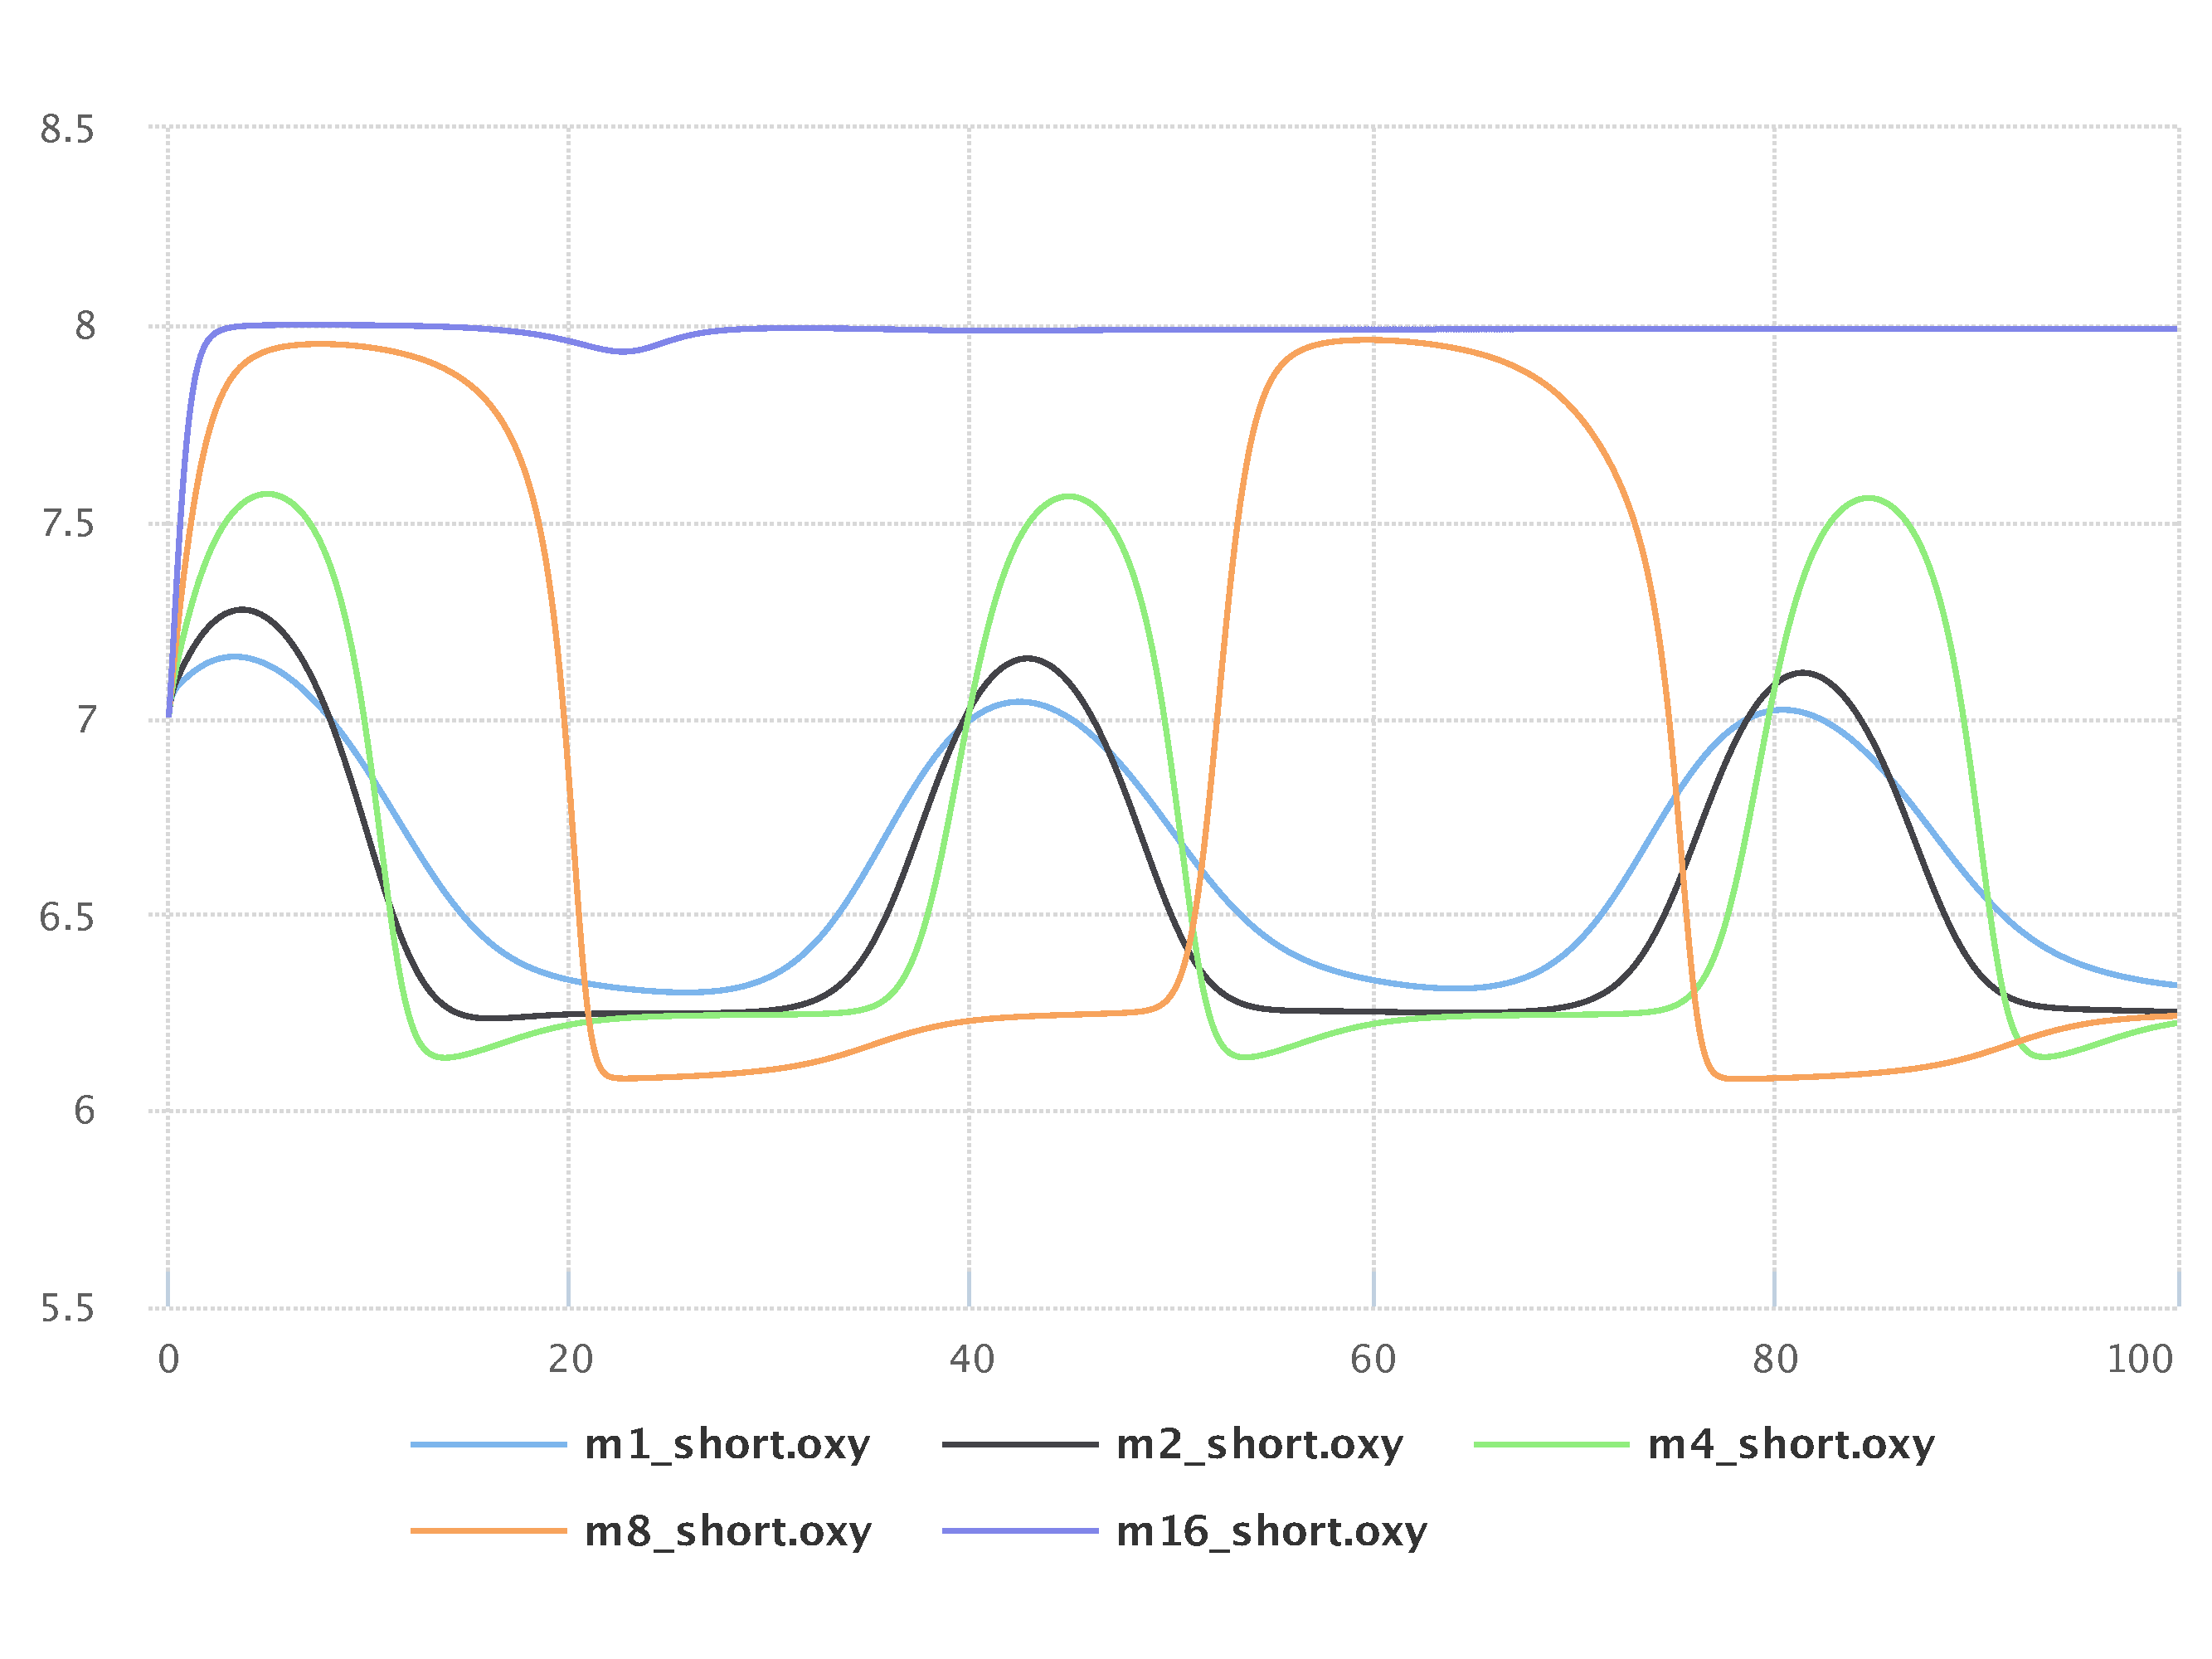
\includegraphics[width=0.75\textwidth]{swt-fig1.pdf}
  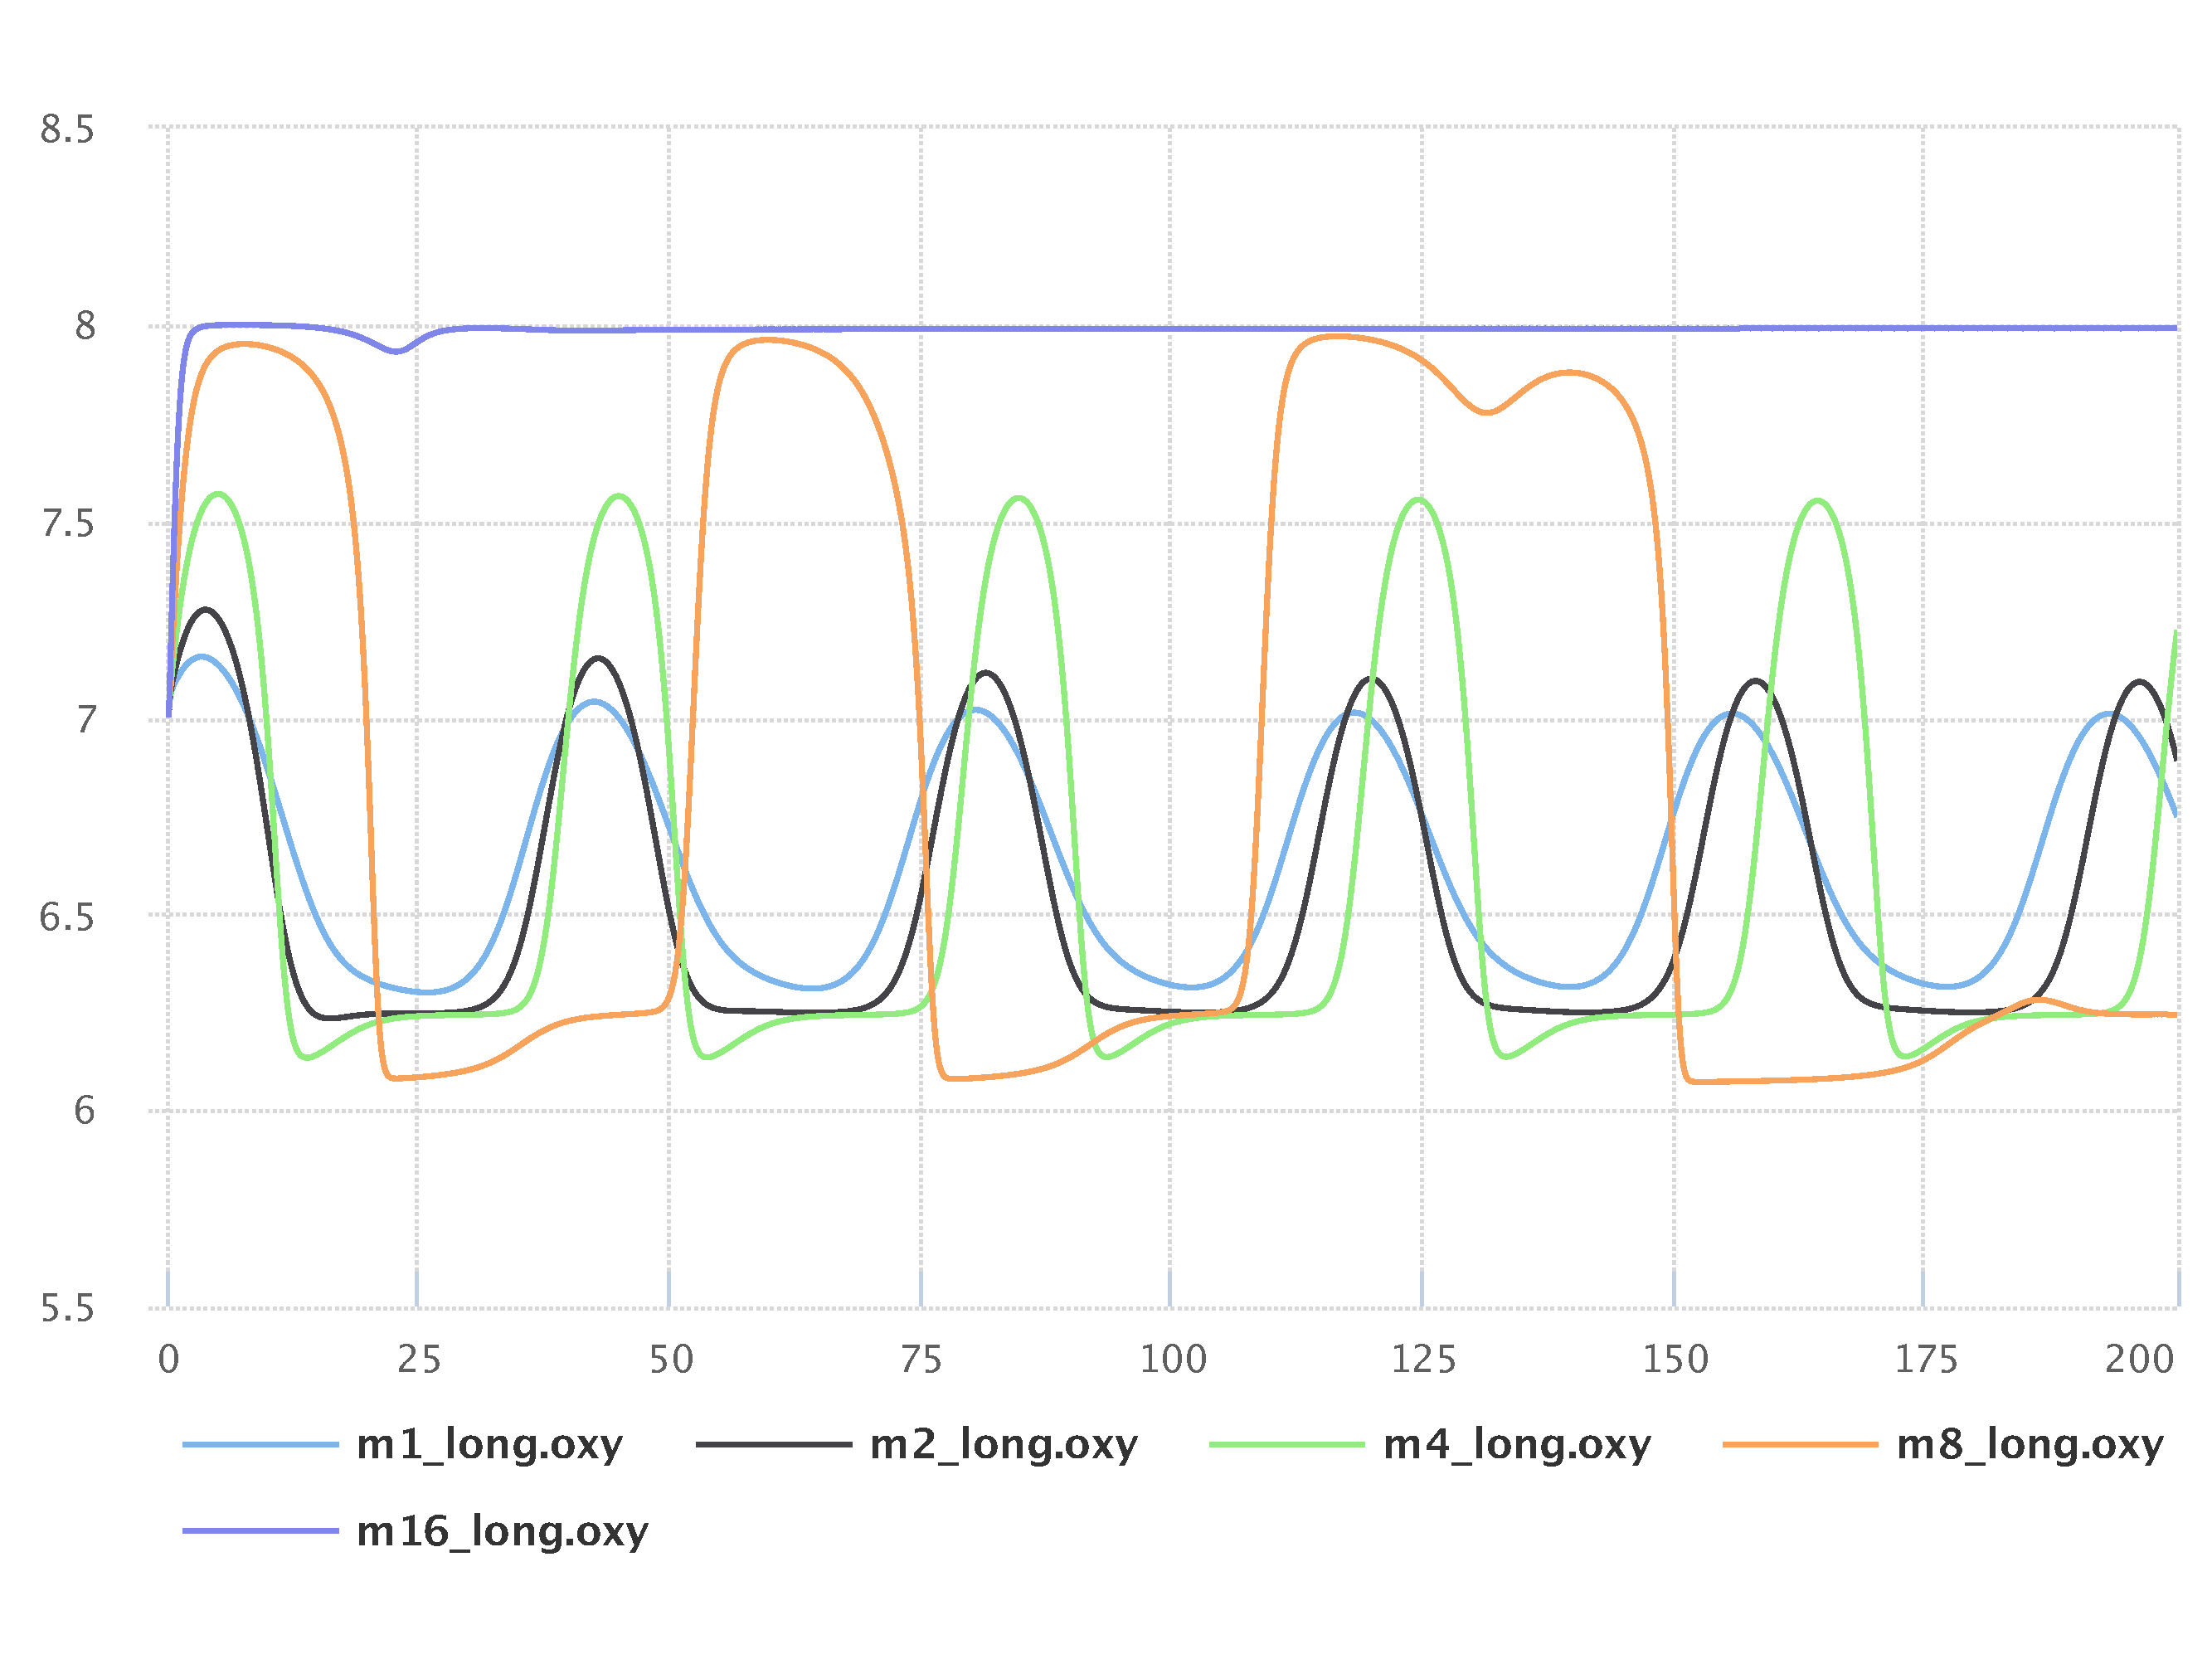
\includegraphics[width=0.75\textwidth]{swt-fig2.pdf}
  \caption{Demonstrating exchangeability of COMBINE archives containing SBML and SED--ML. The respiratory oscillation case study in Fig \ref{fig:hill} was exported to a COMBINE archive from Tellurium, imported into the SED--ML Web Tools \cite{bergmann2017sed}, and used to generate plots to verify that the simulation results were identical to Fig \ref{fig:hill}. The COMBINE archive used to create this example can be found online \cite{wolfhillstudy}. }
  \label{fig:swt}
\end{figure}

\clearpage

\begin{figure}
  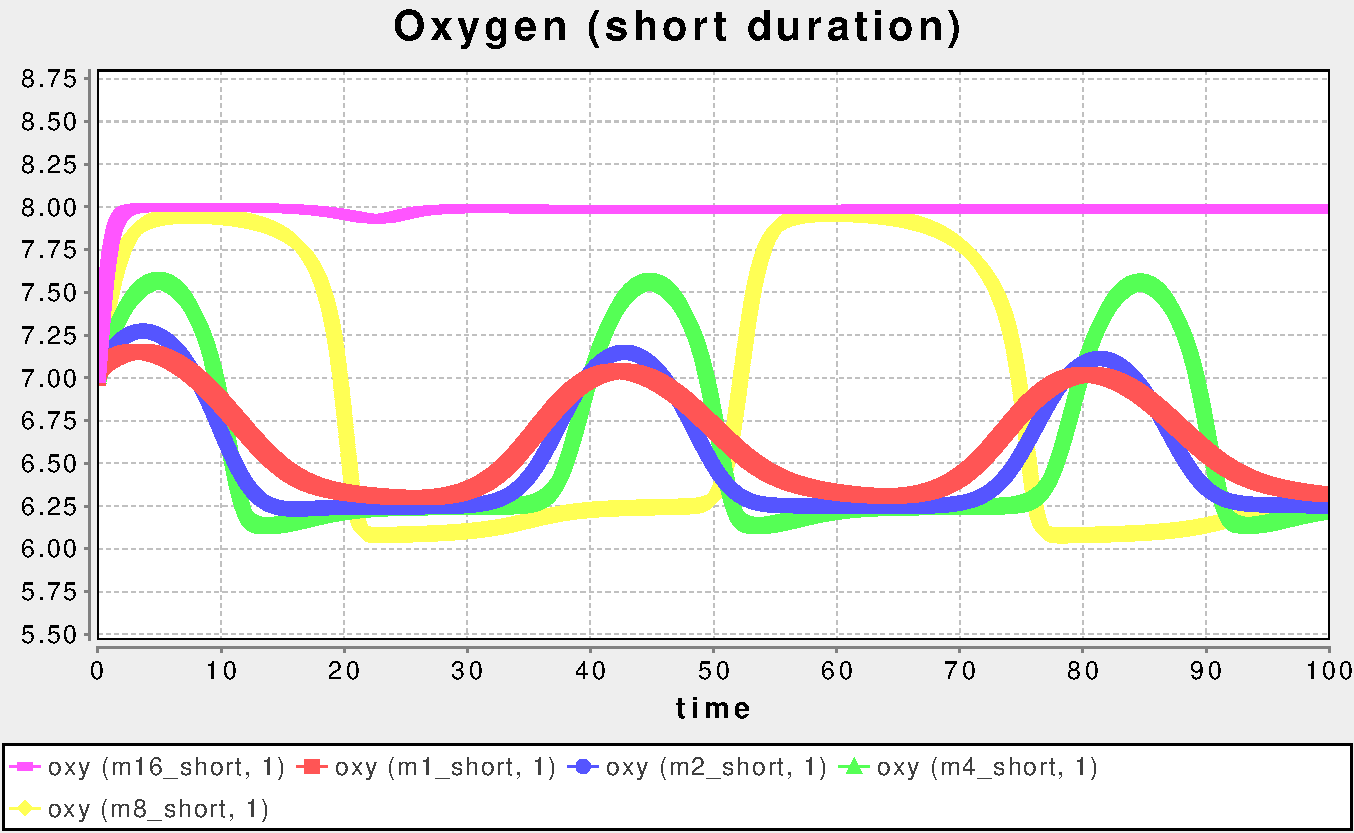
\includegraphics[width=0.9\textwidth]{wolf-ibiosim-short.pdf}
  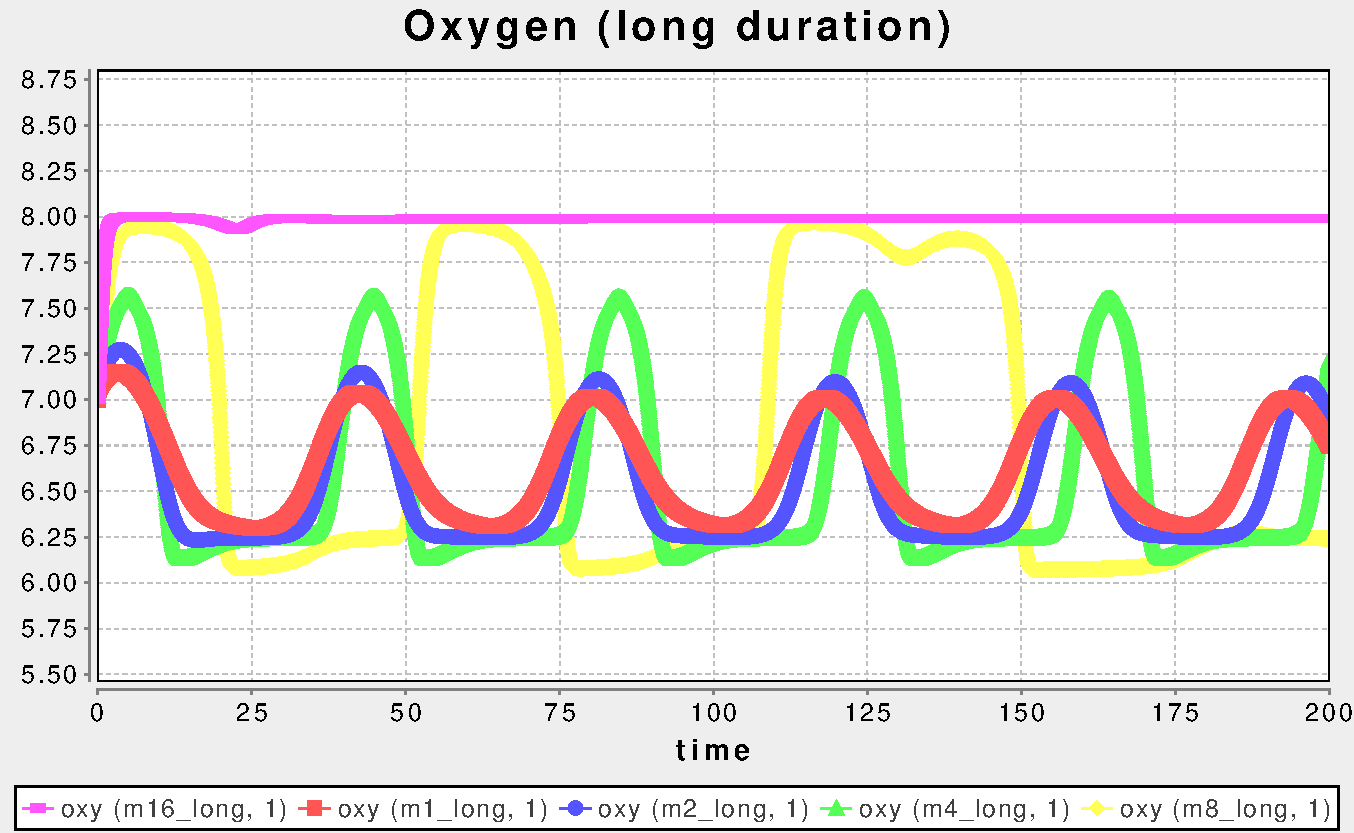
\includegraphics[width=0.9\textwidth]{wolf-ibiosim-long.pdf}
  \caption{A second test of exchangeability. To demonstrate exchangeability between multiple tools, the same Hill coefficient case study as shown in Fig \ref{fig:swt} was exported to iBioSim \cite{myers2009ibiosim} and used to produce identical plots. This shows that COMBINE archives are sufficiently flexible to be exchanged between different tools, despite the limited number of tools which currently support the format. }
  \label{fig:ibiosim}
\end{figure}

\clearpage

\begin{figure}
  \begin{subfigure}{0.5\textwidth}
    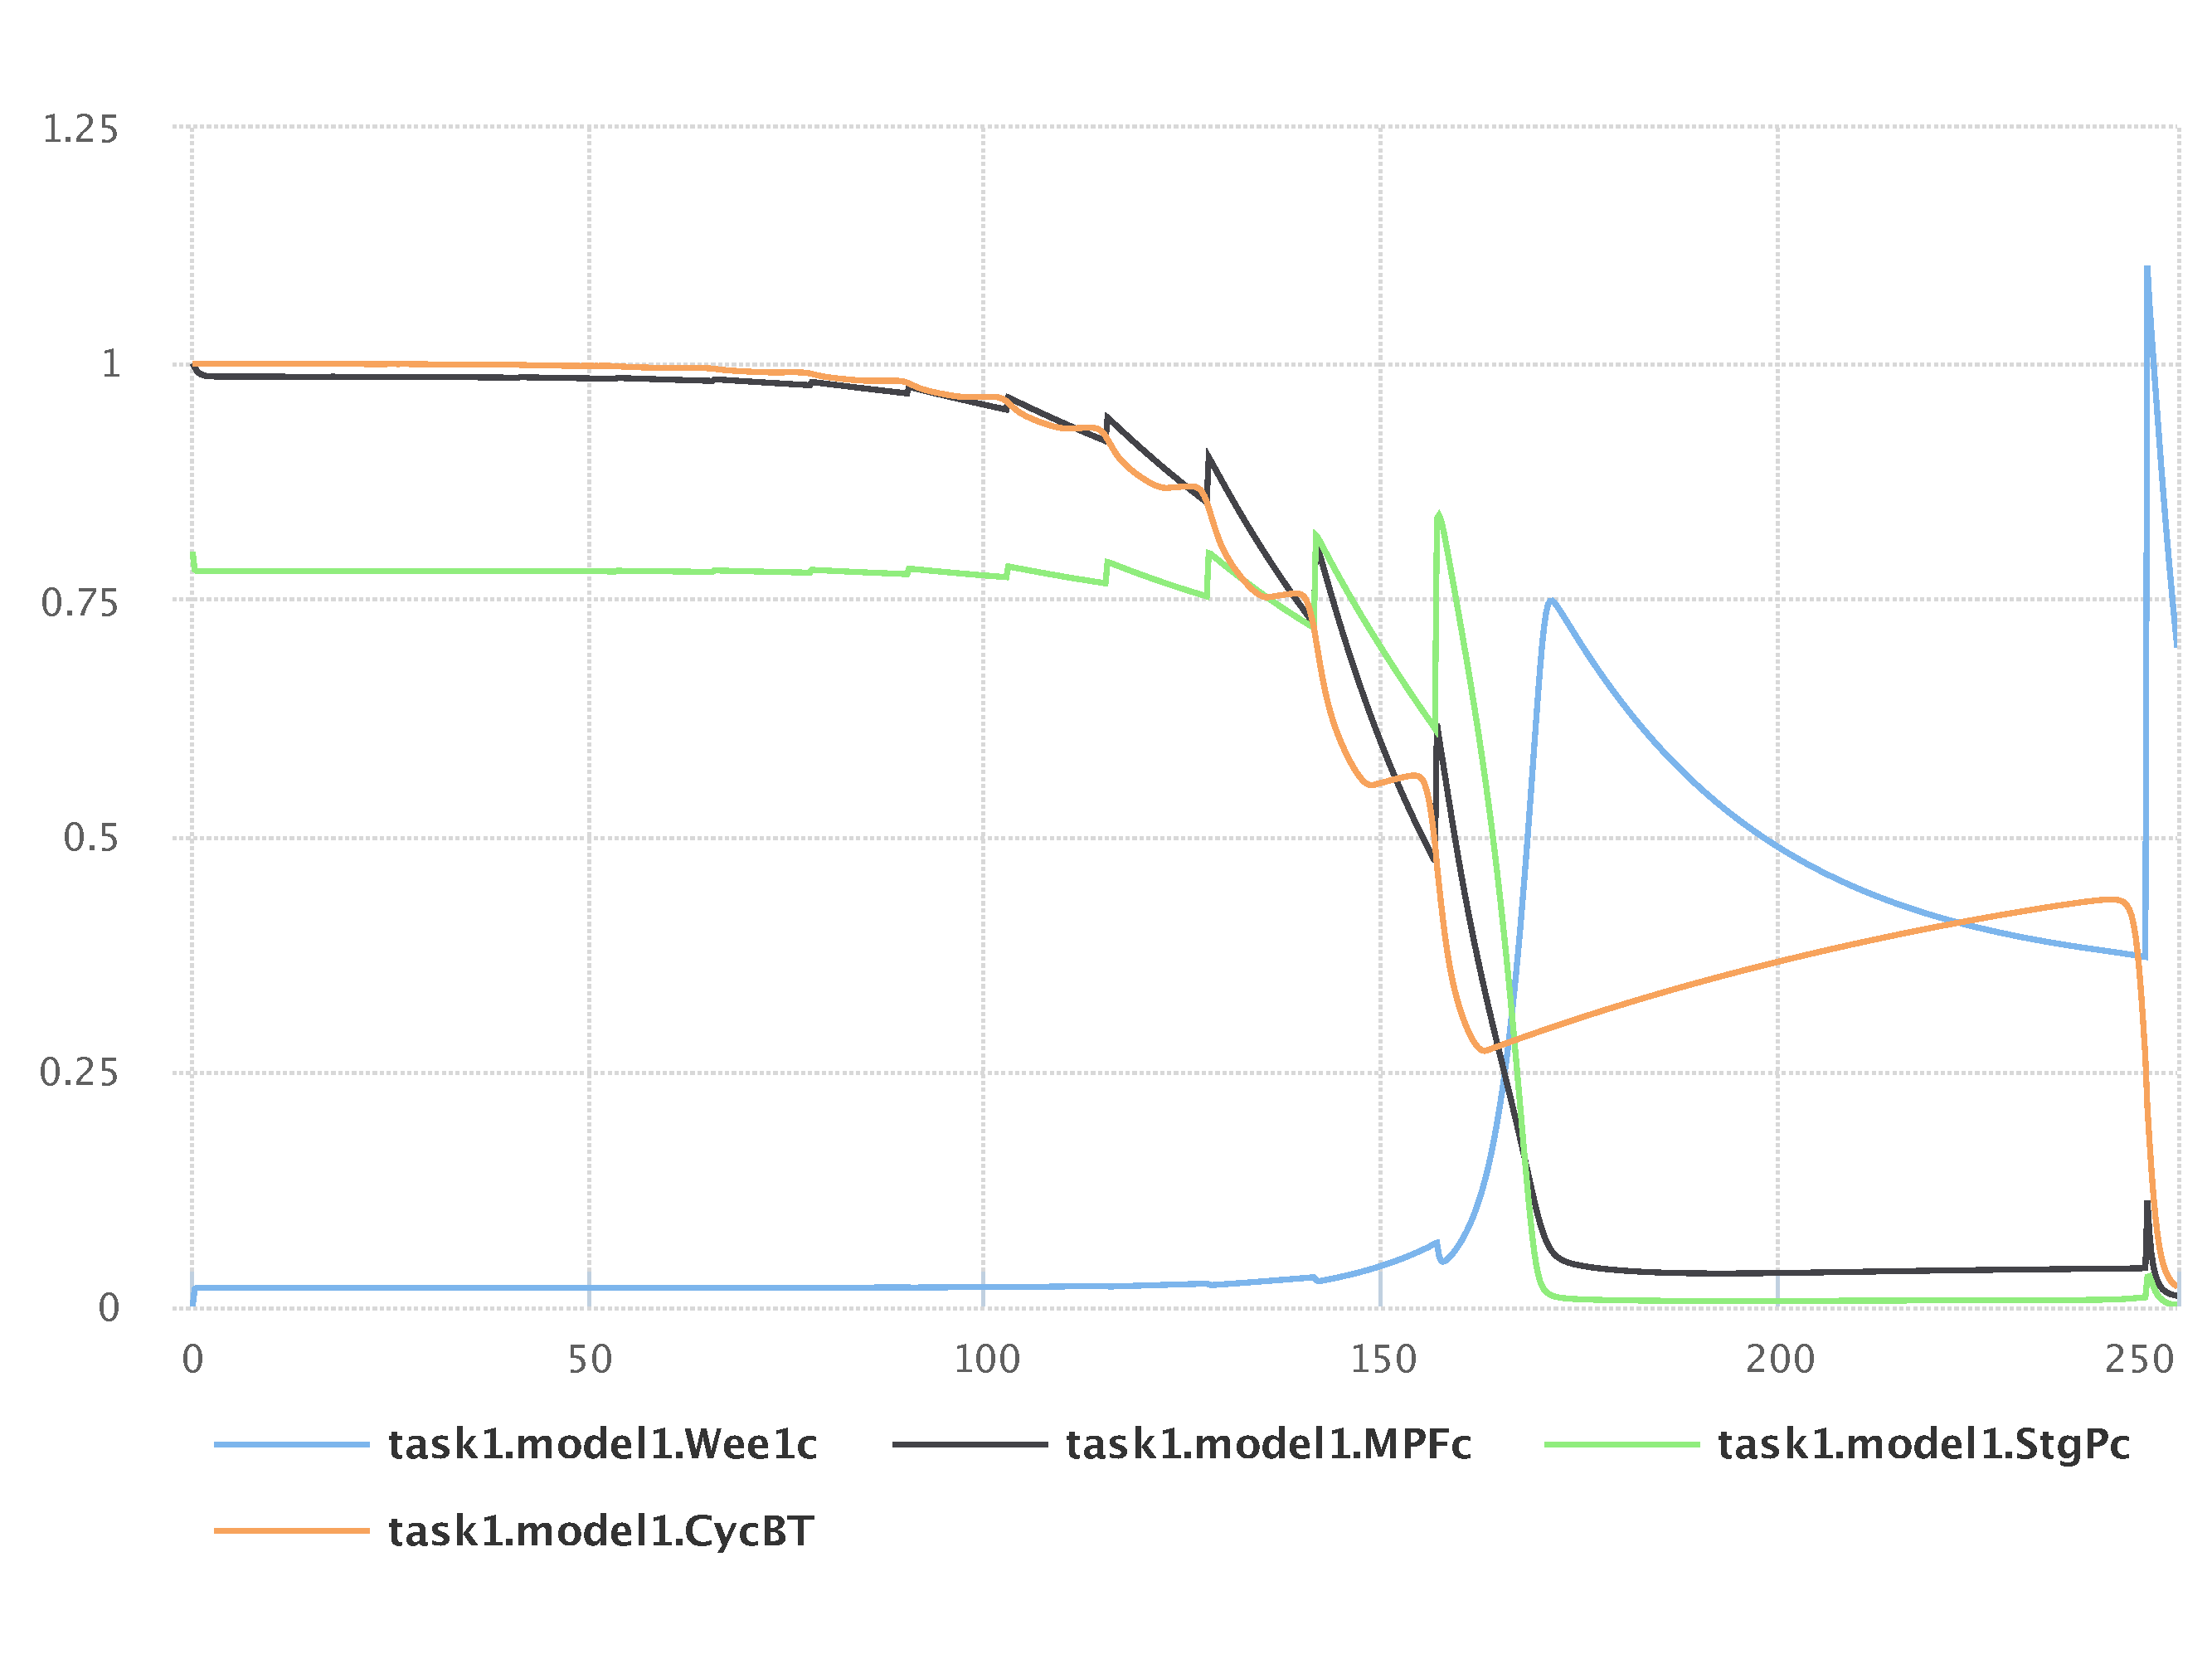
\includegraphics[width=0.75\textwidth]{swt-calzone1.pdf}
    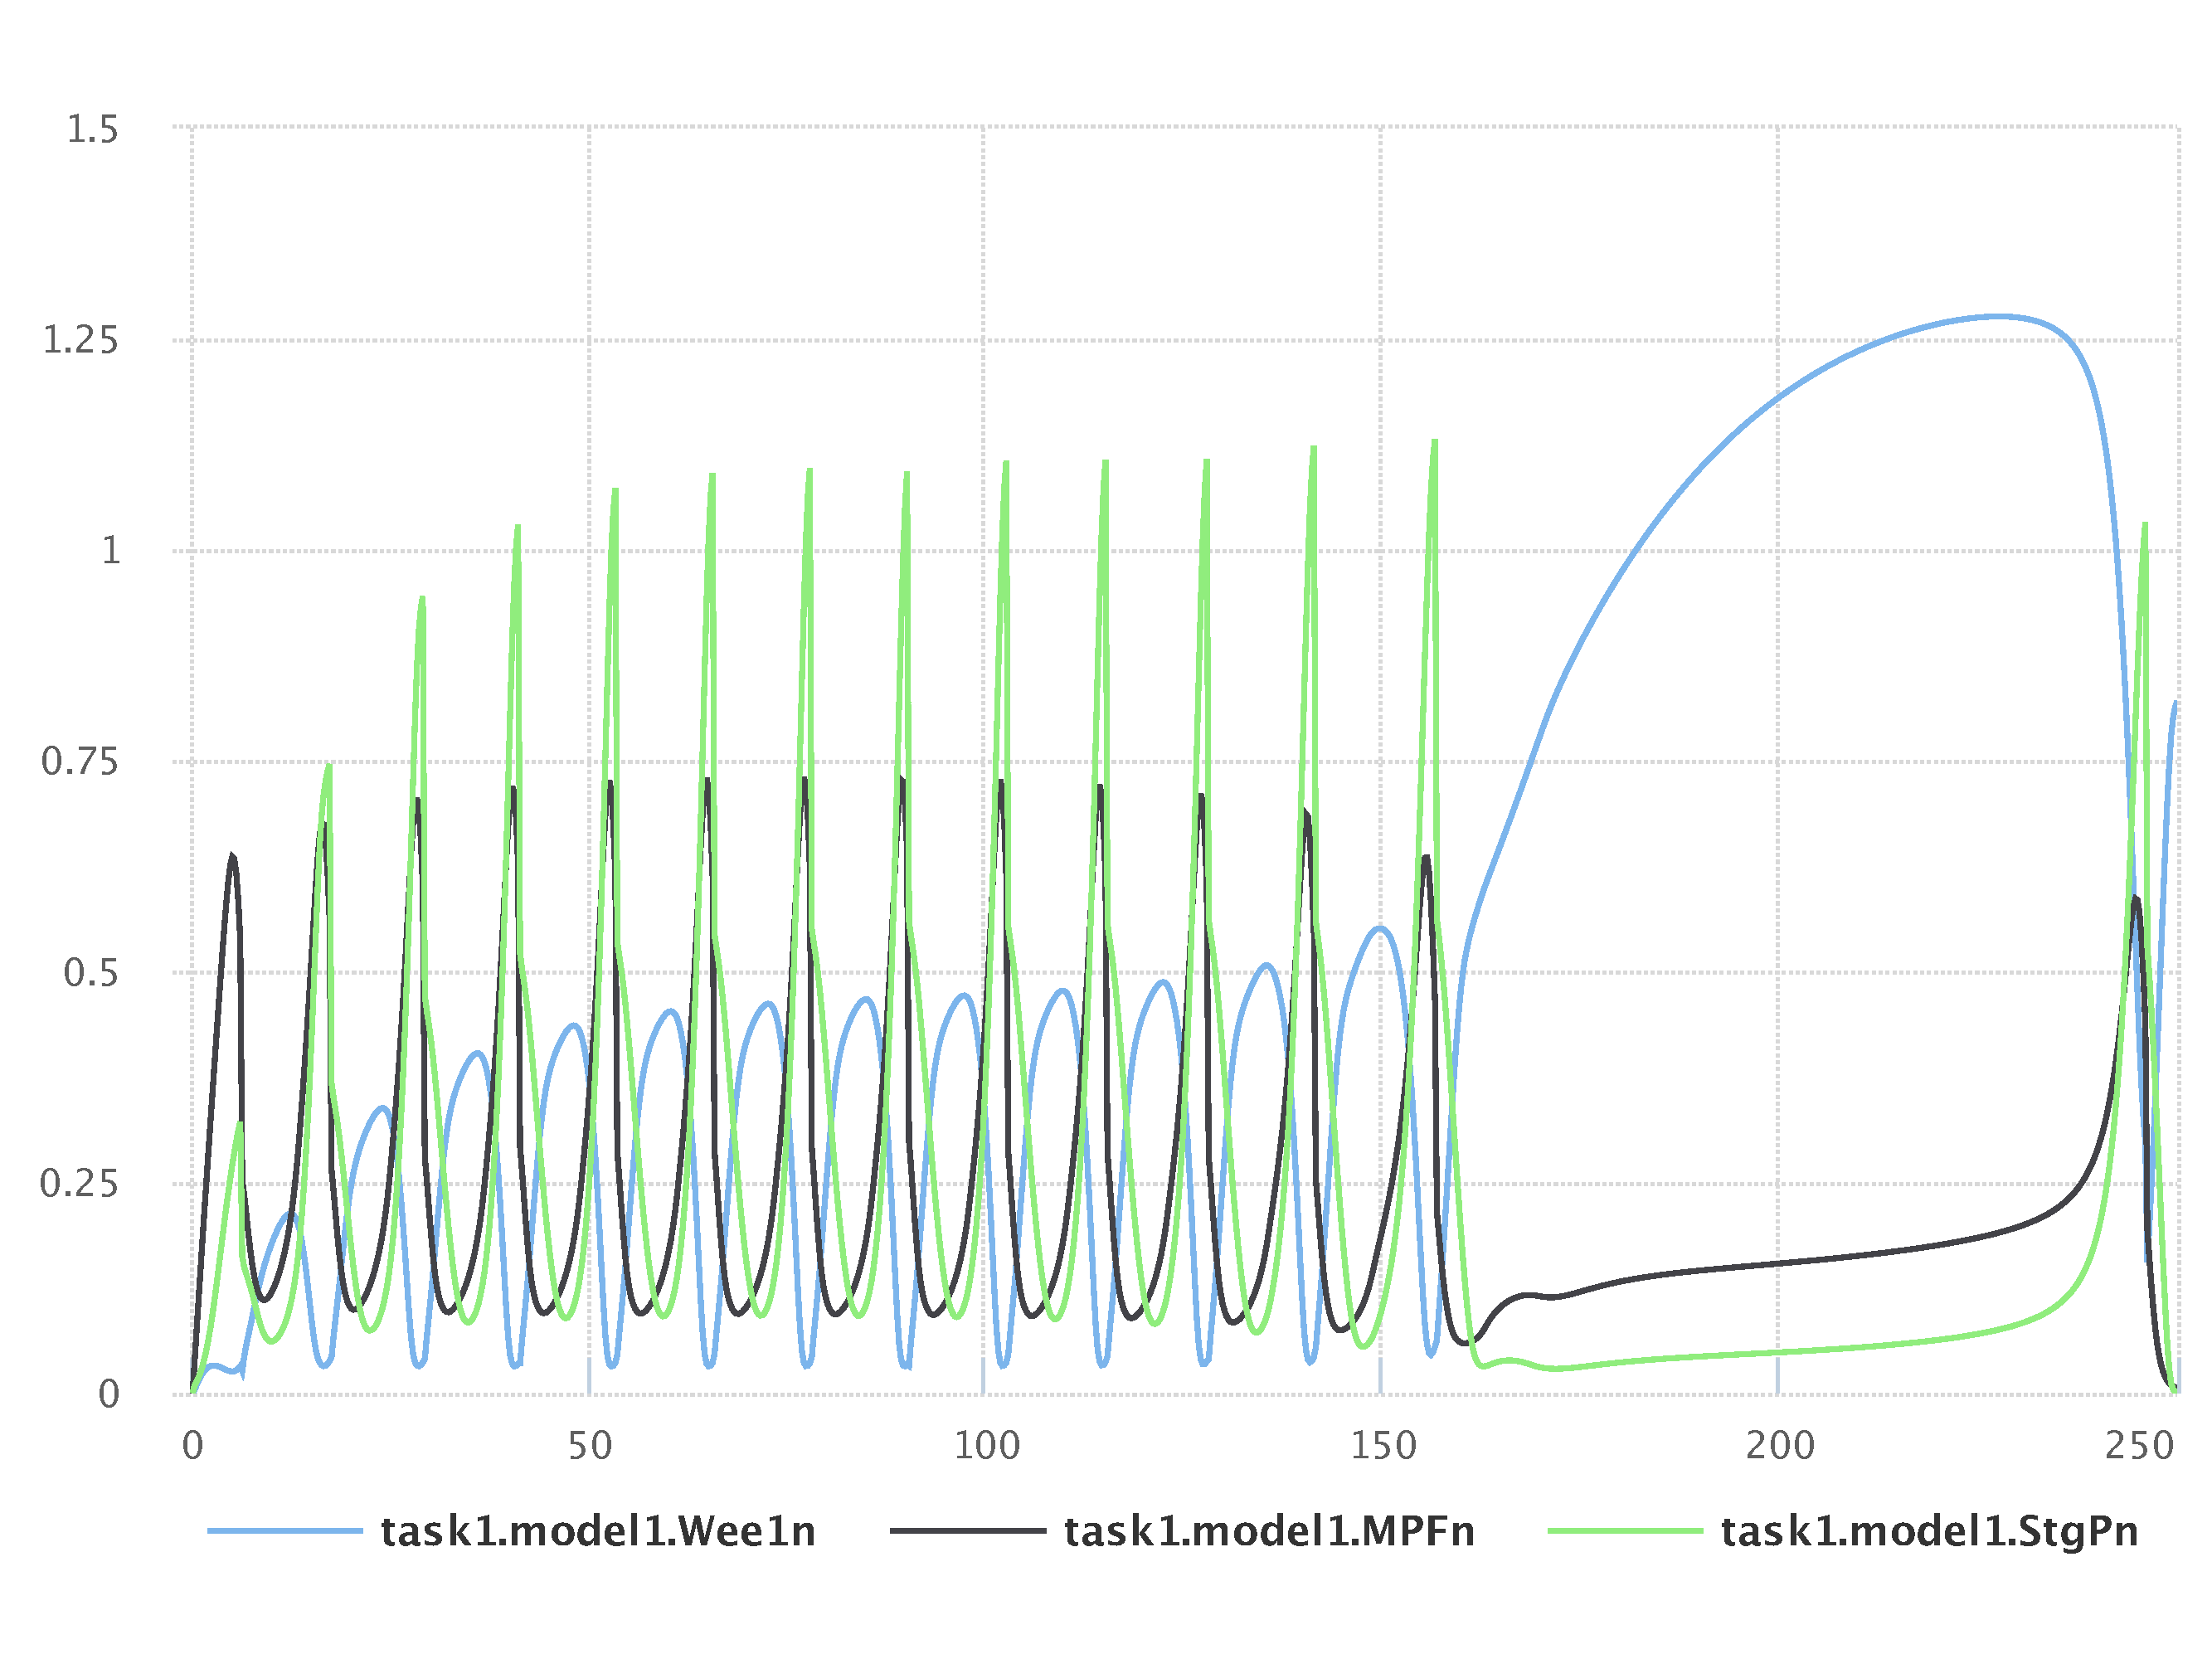
\includegraphics[width=0.75\textwidth]{swt-calzone2.pdf}
    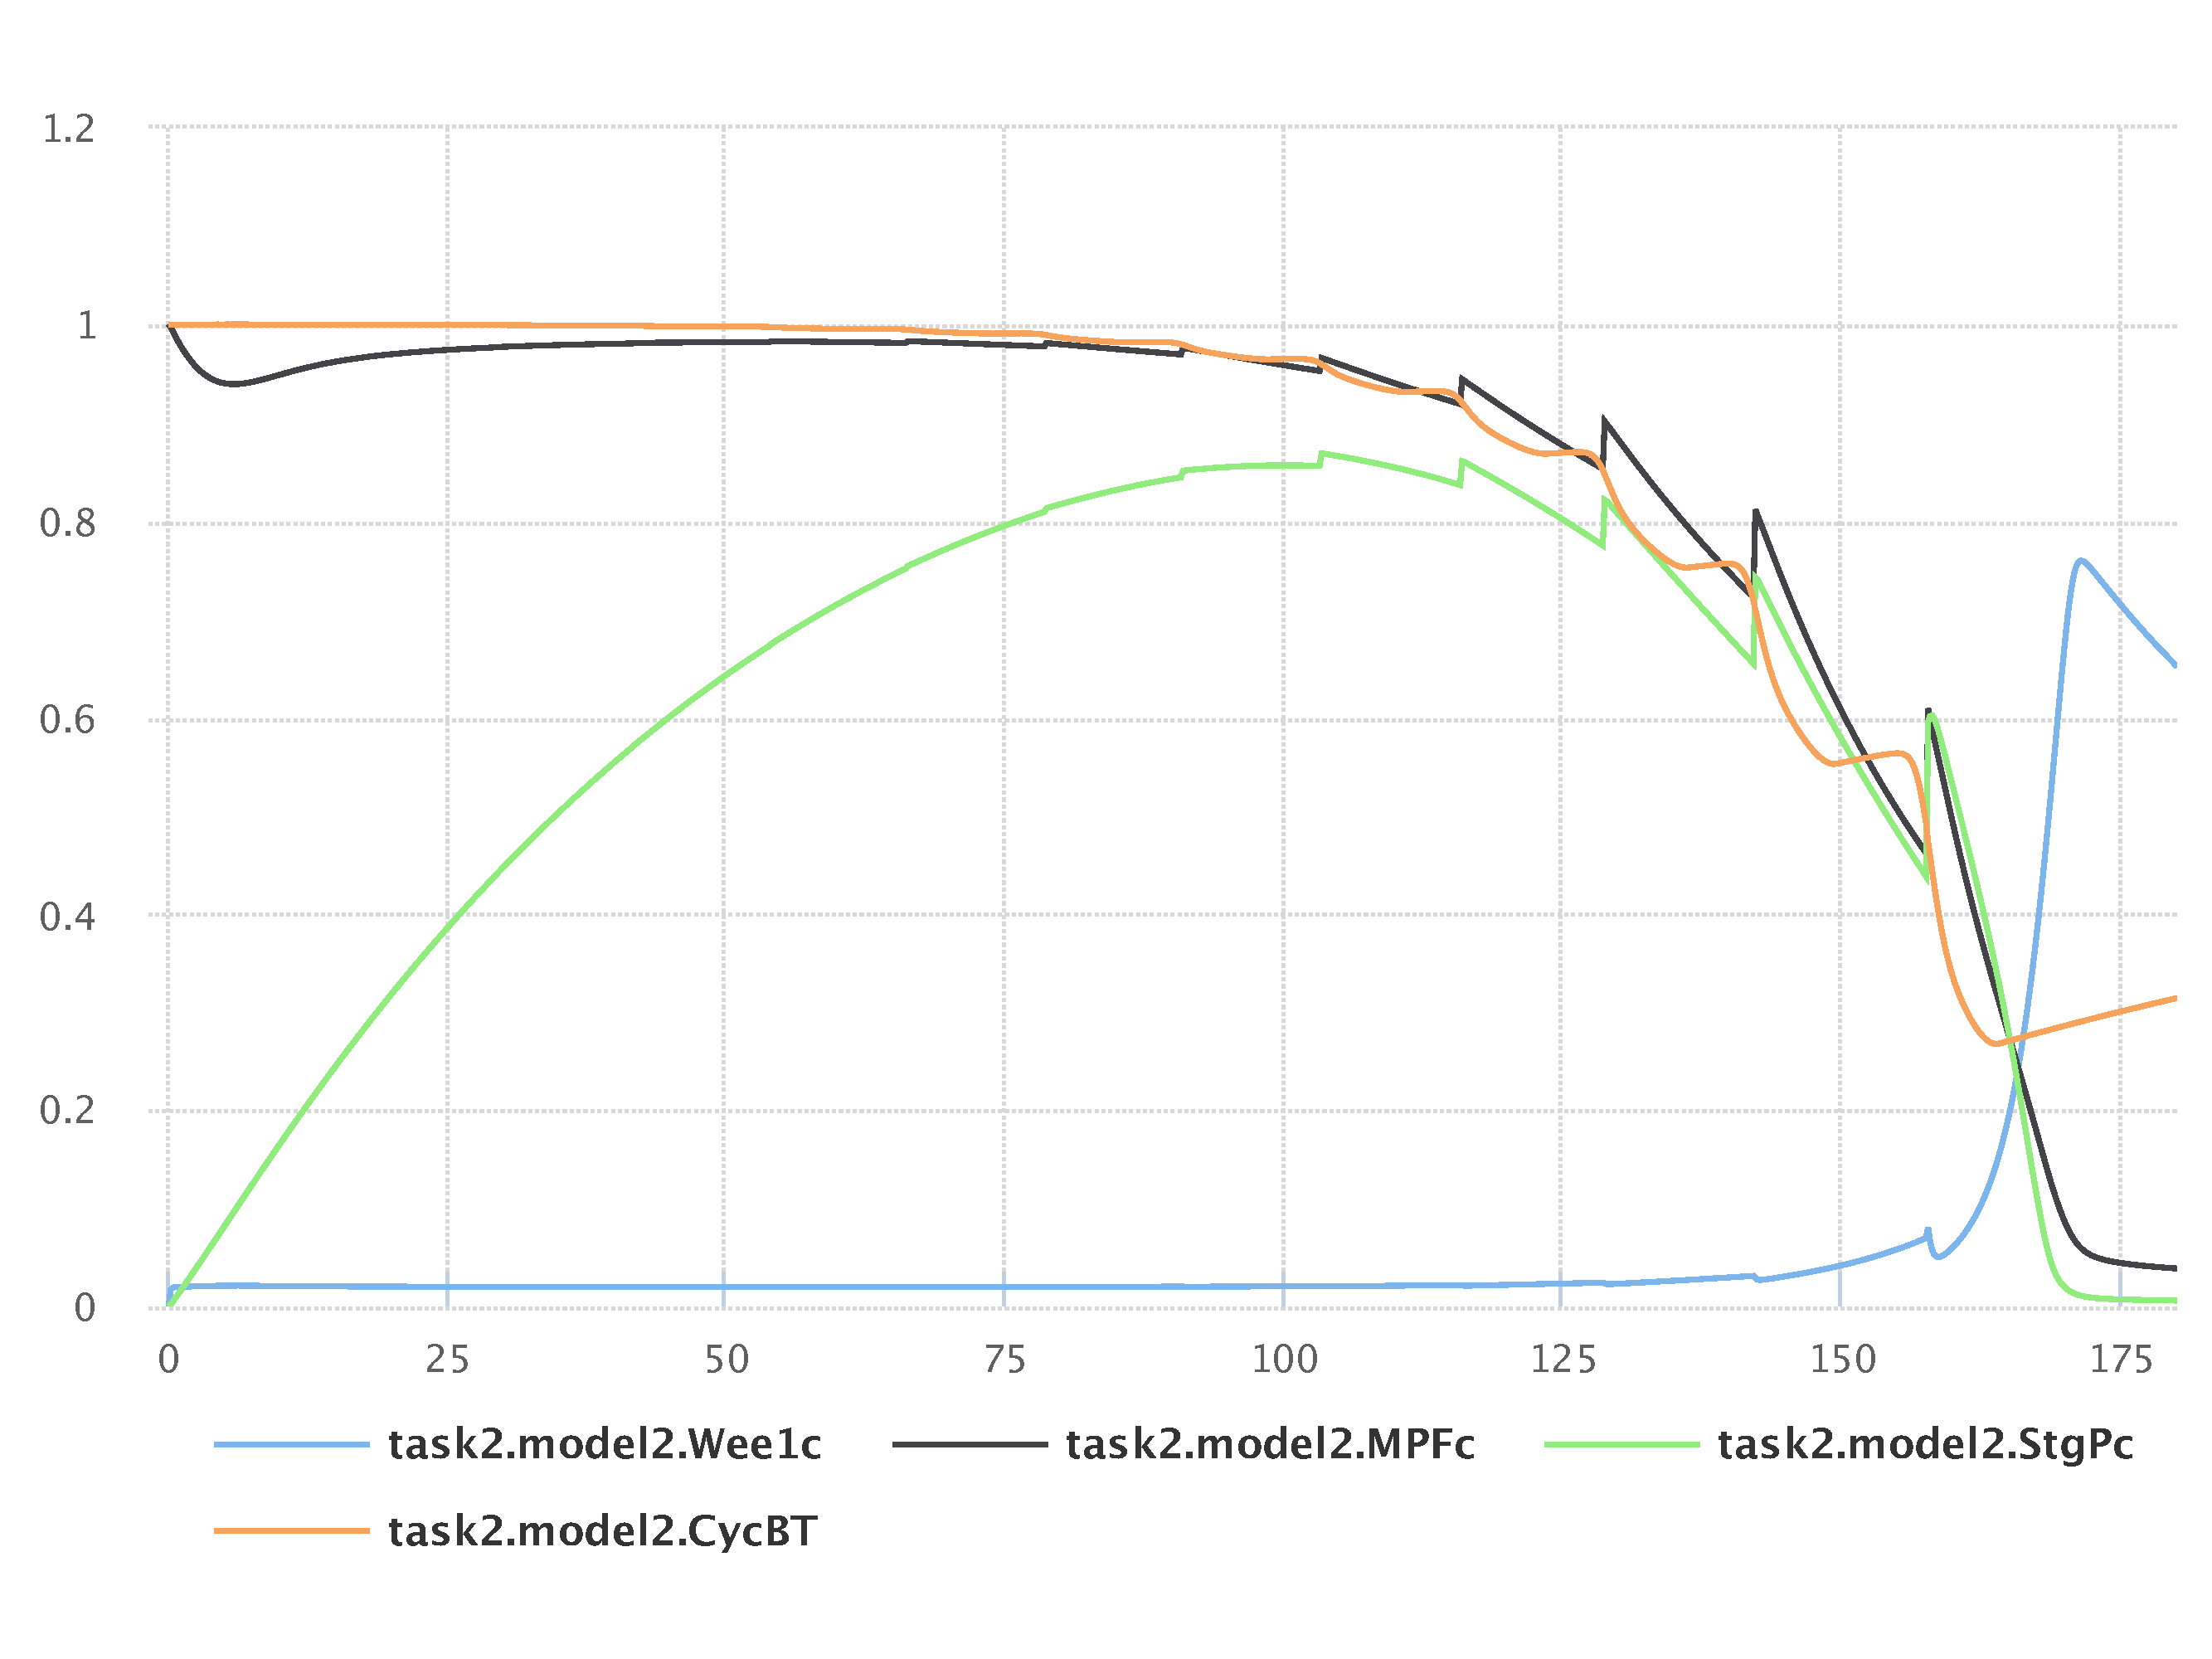
\includegraphics[width=0.75\textwidth]{swt-calzone3.pdf}
  \end{subfigure}
  \begin{subfigure}{0.5\textwidth}
    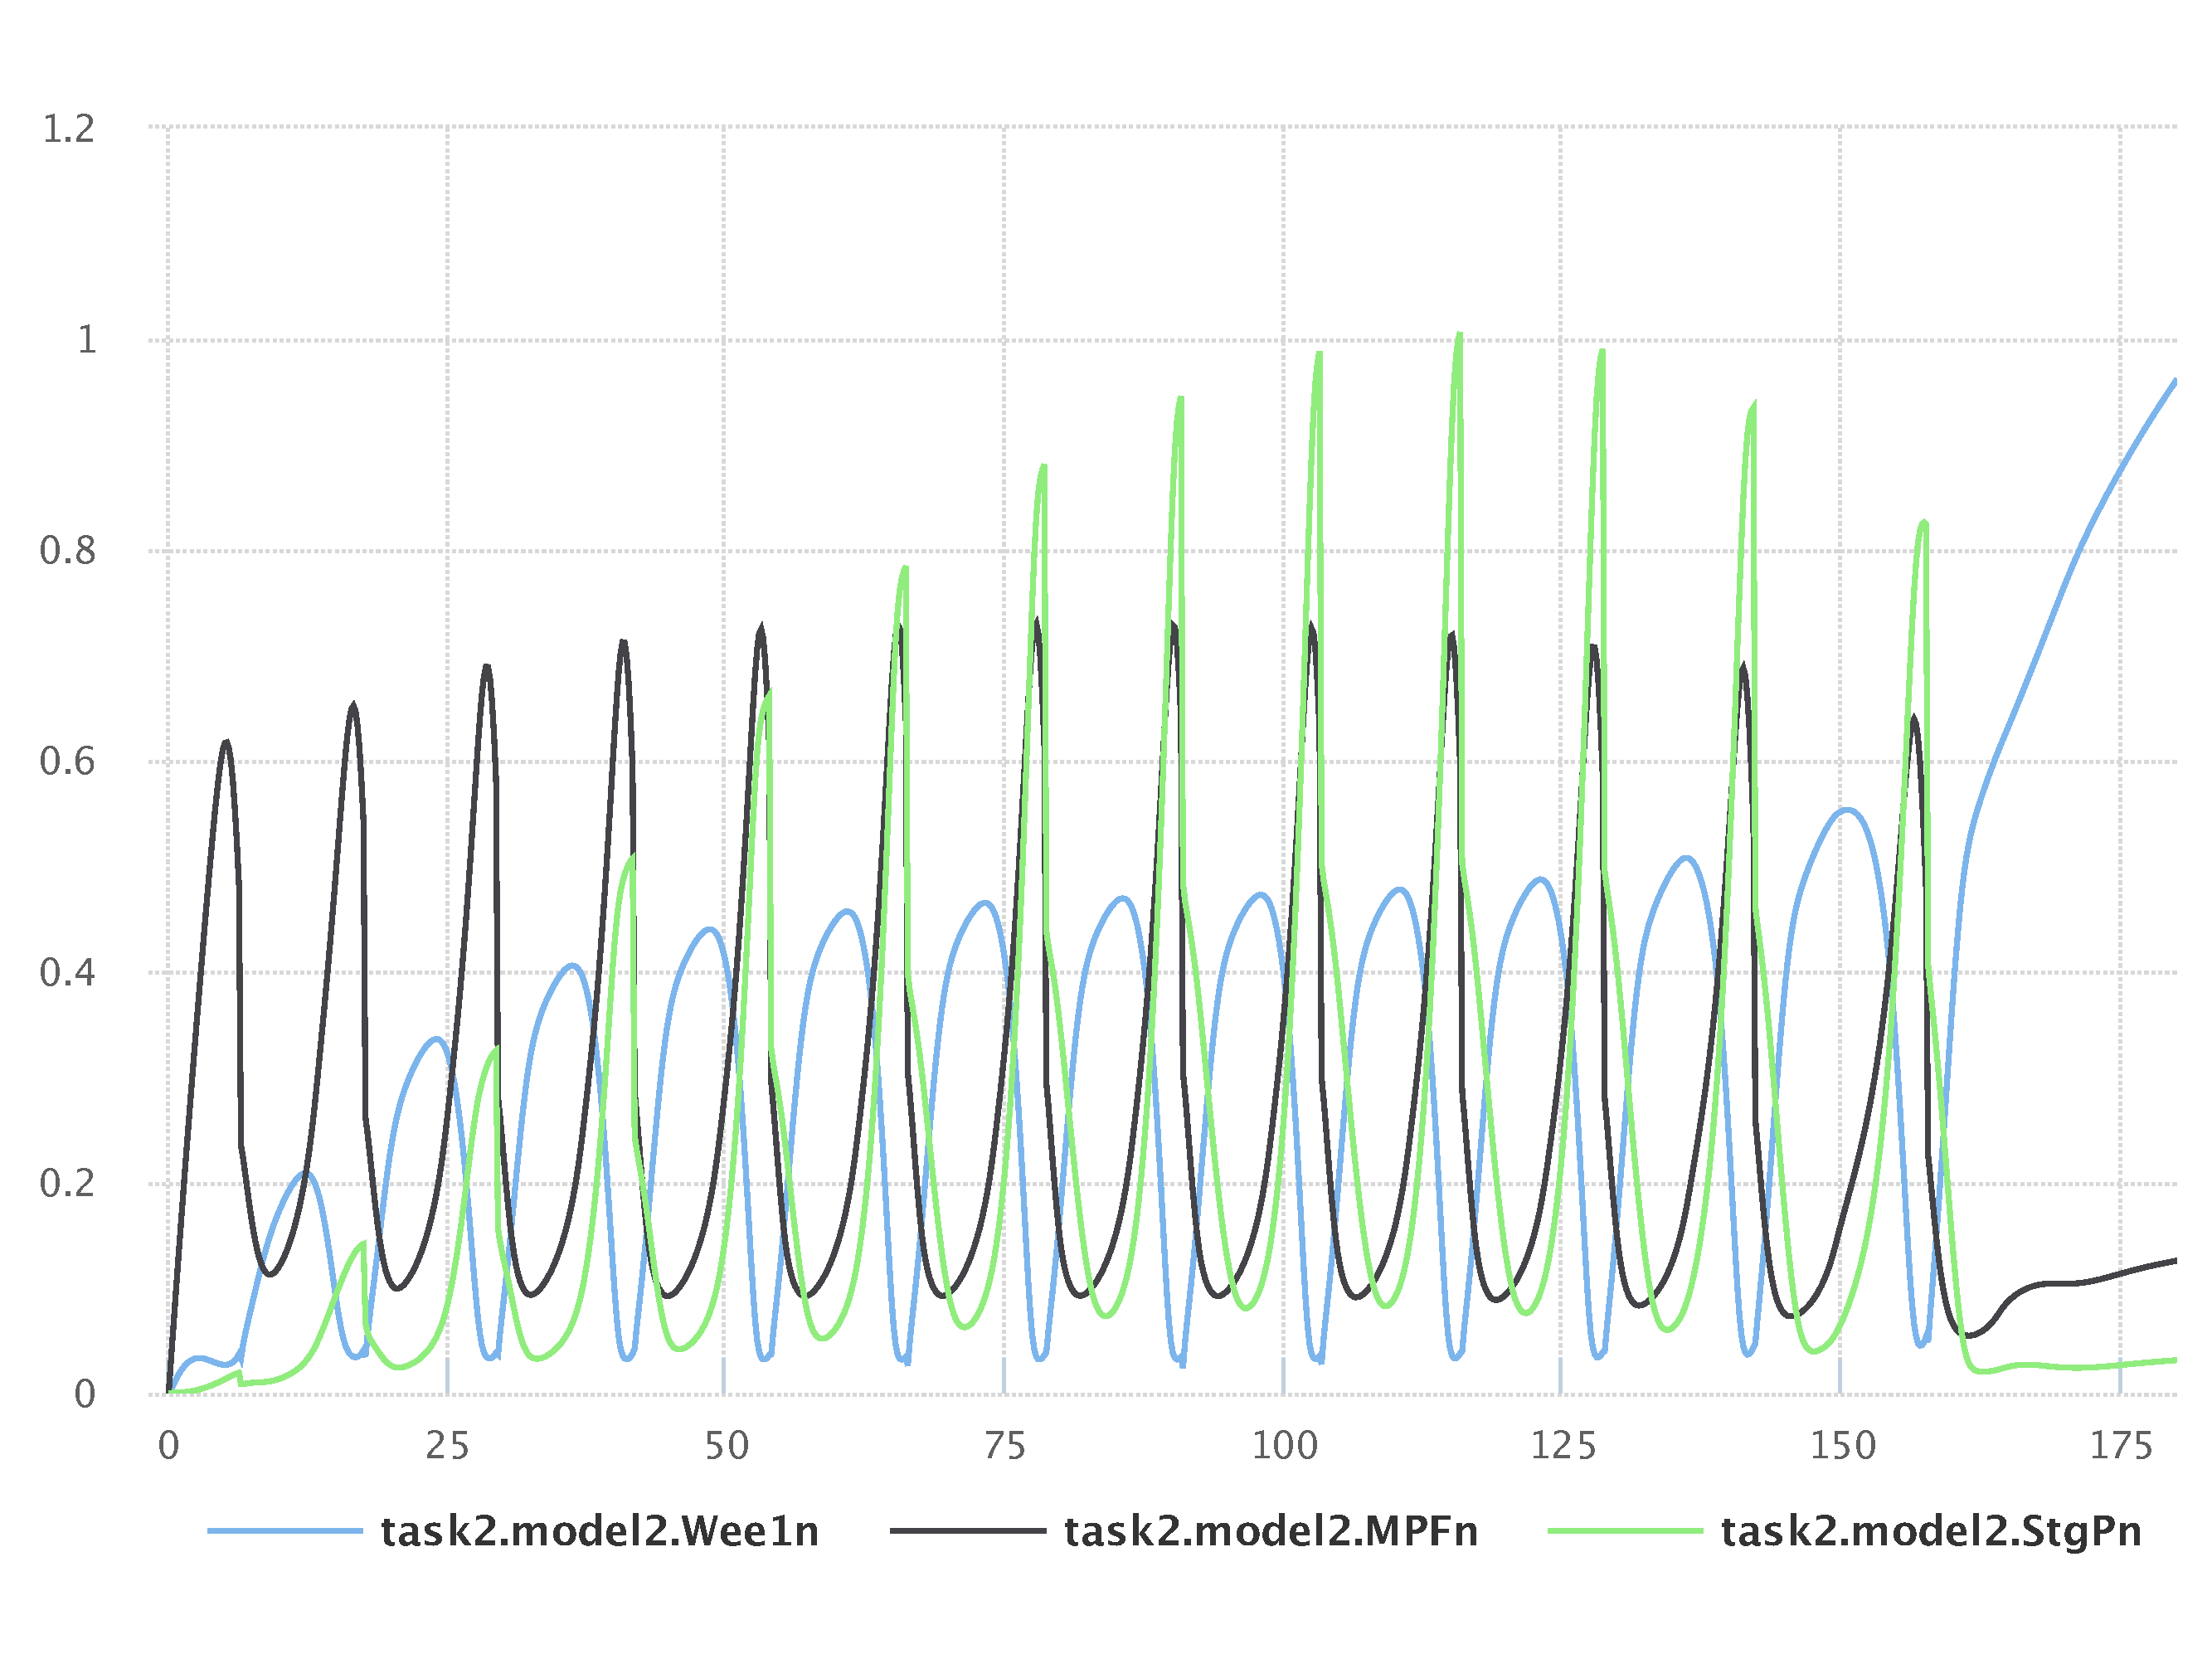
\includegraphics[width=0.75\textwidth]{swt-calzone4.pdf}
    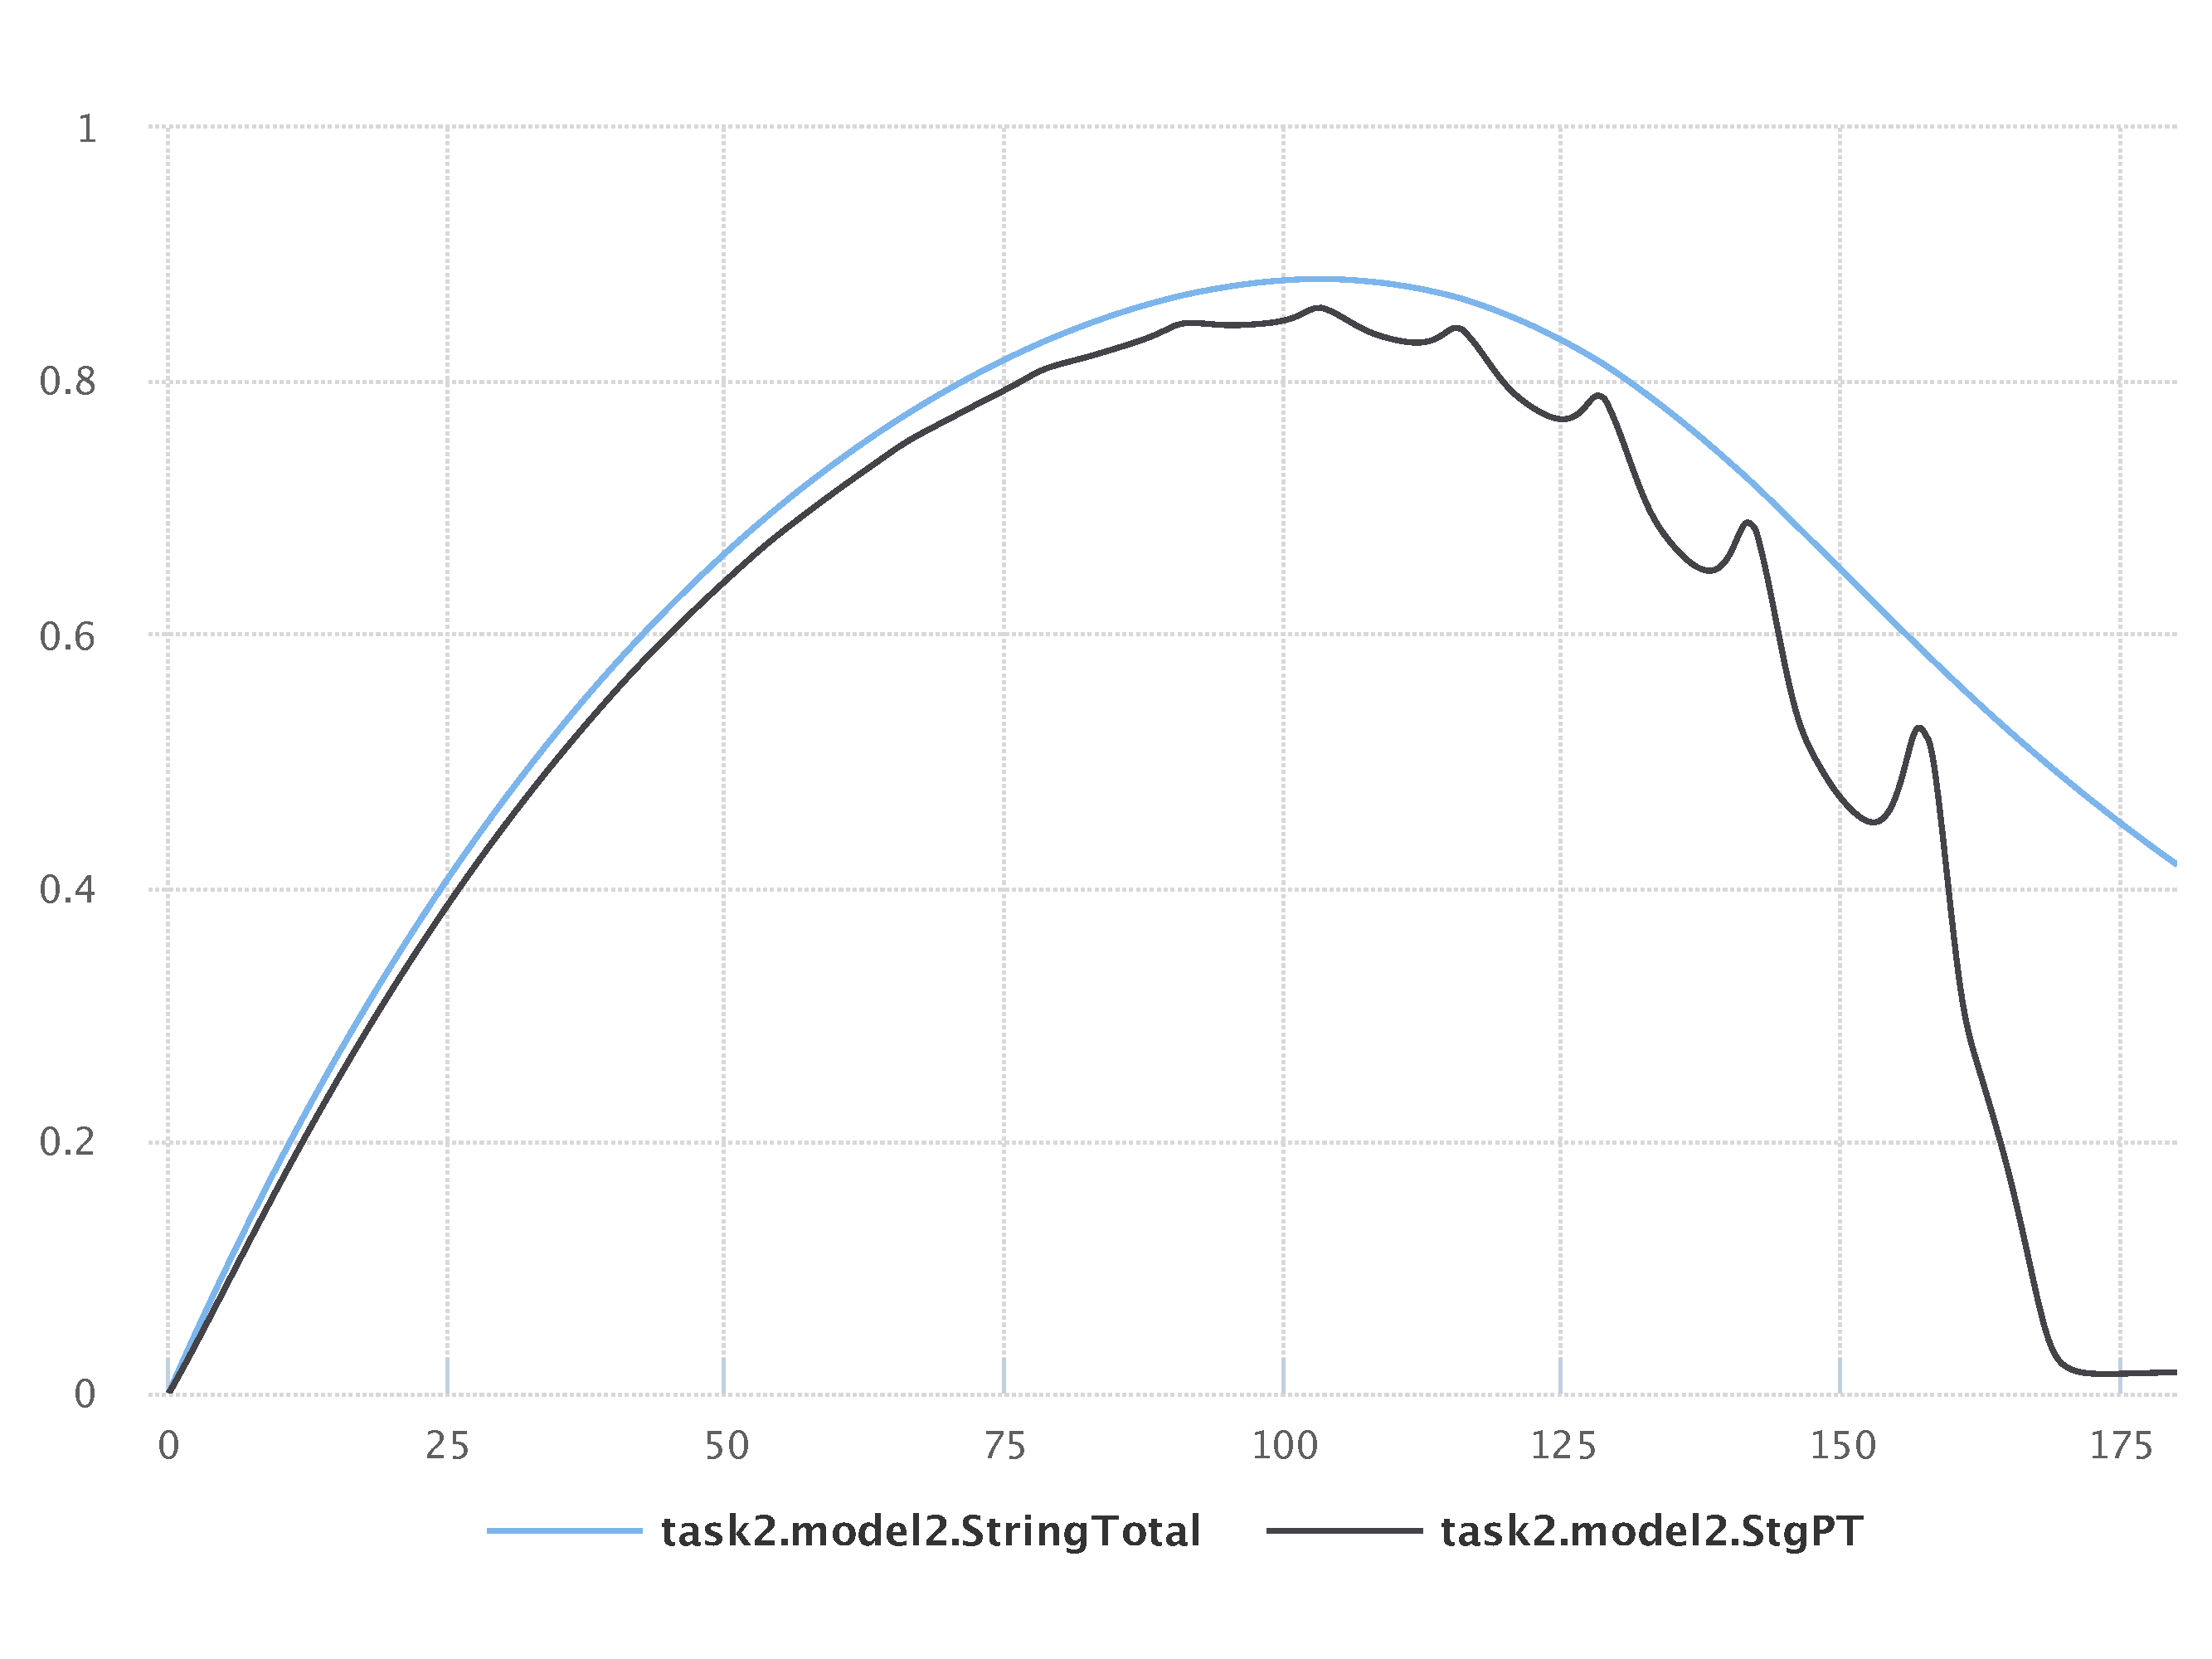
\includegraphics[width=0.75\textwidth]{swt-calzone5.pdf}
    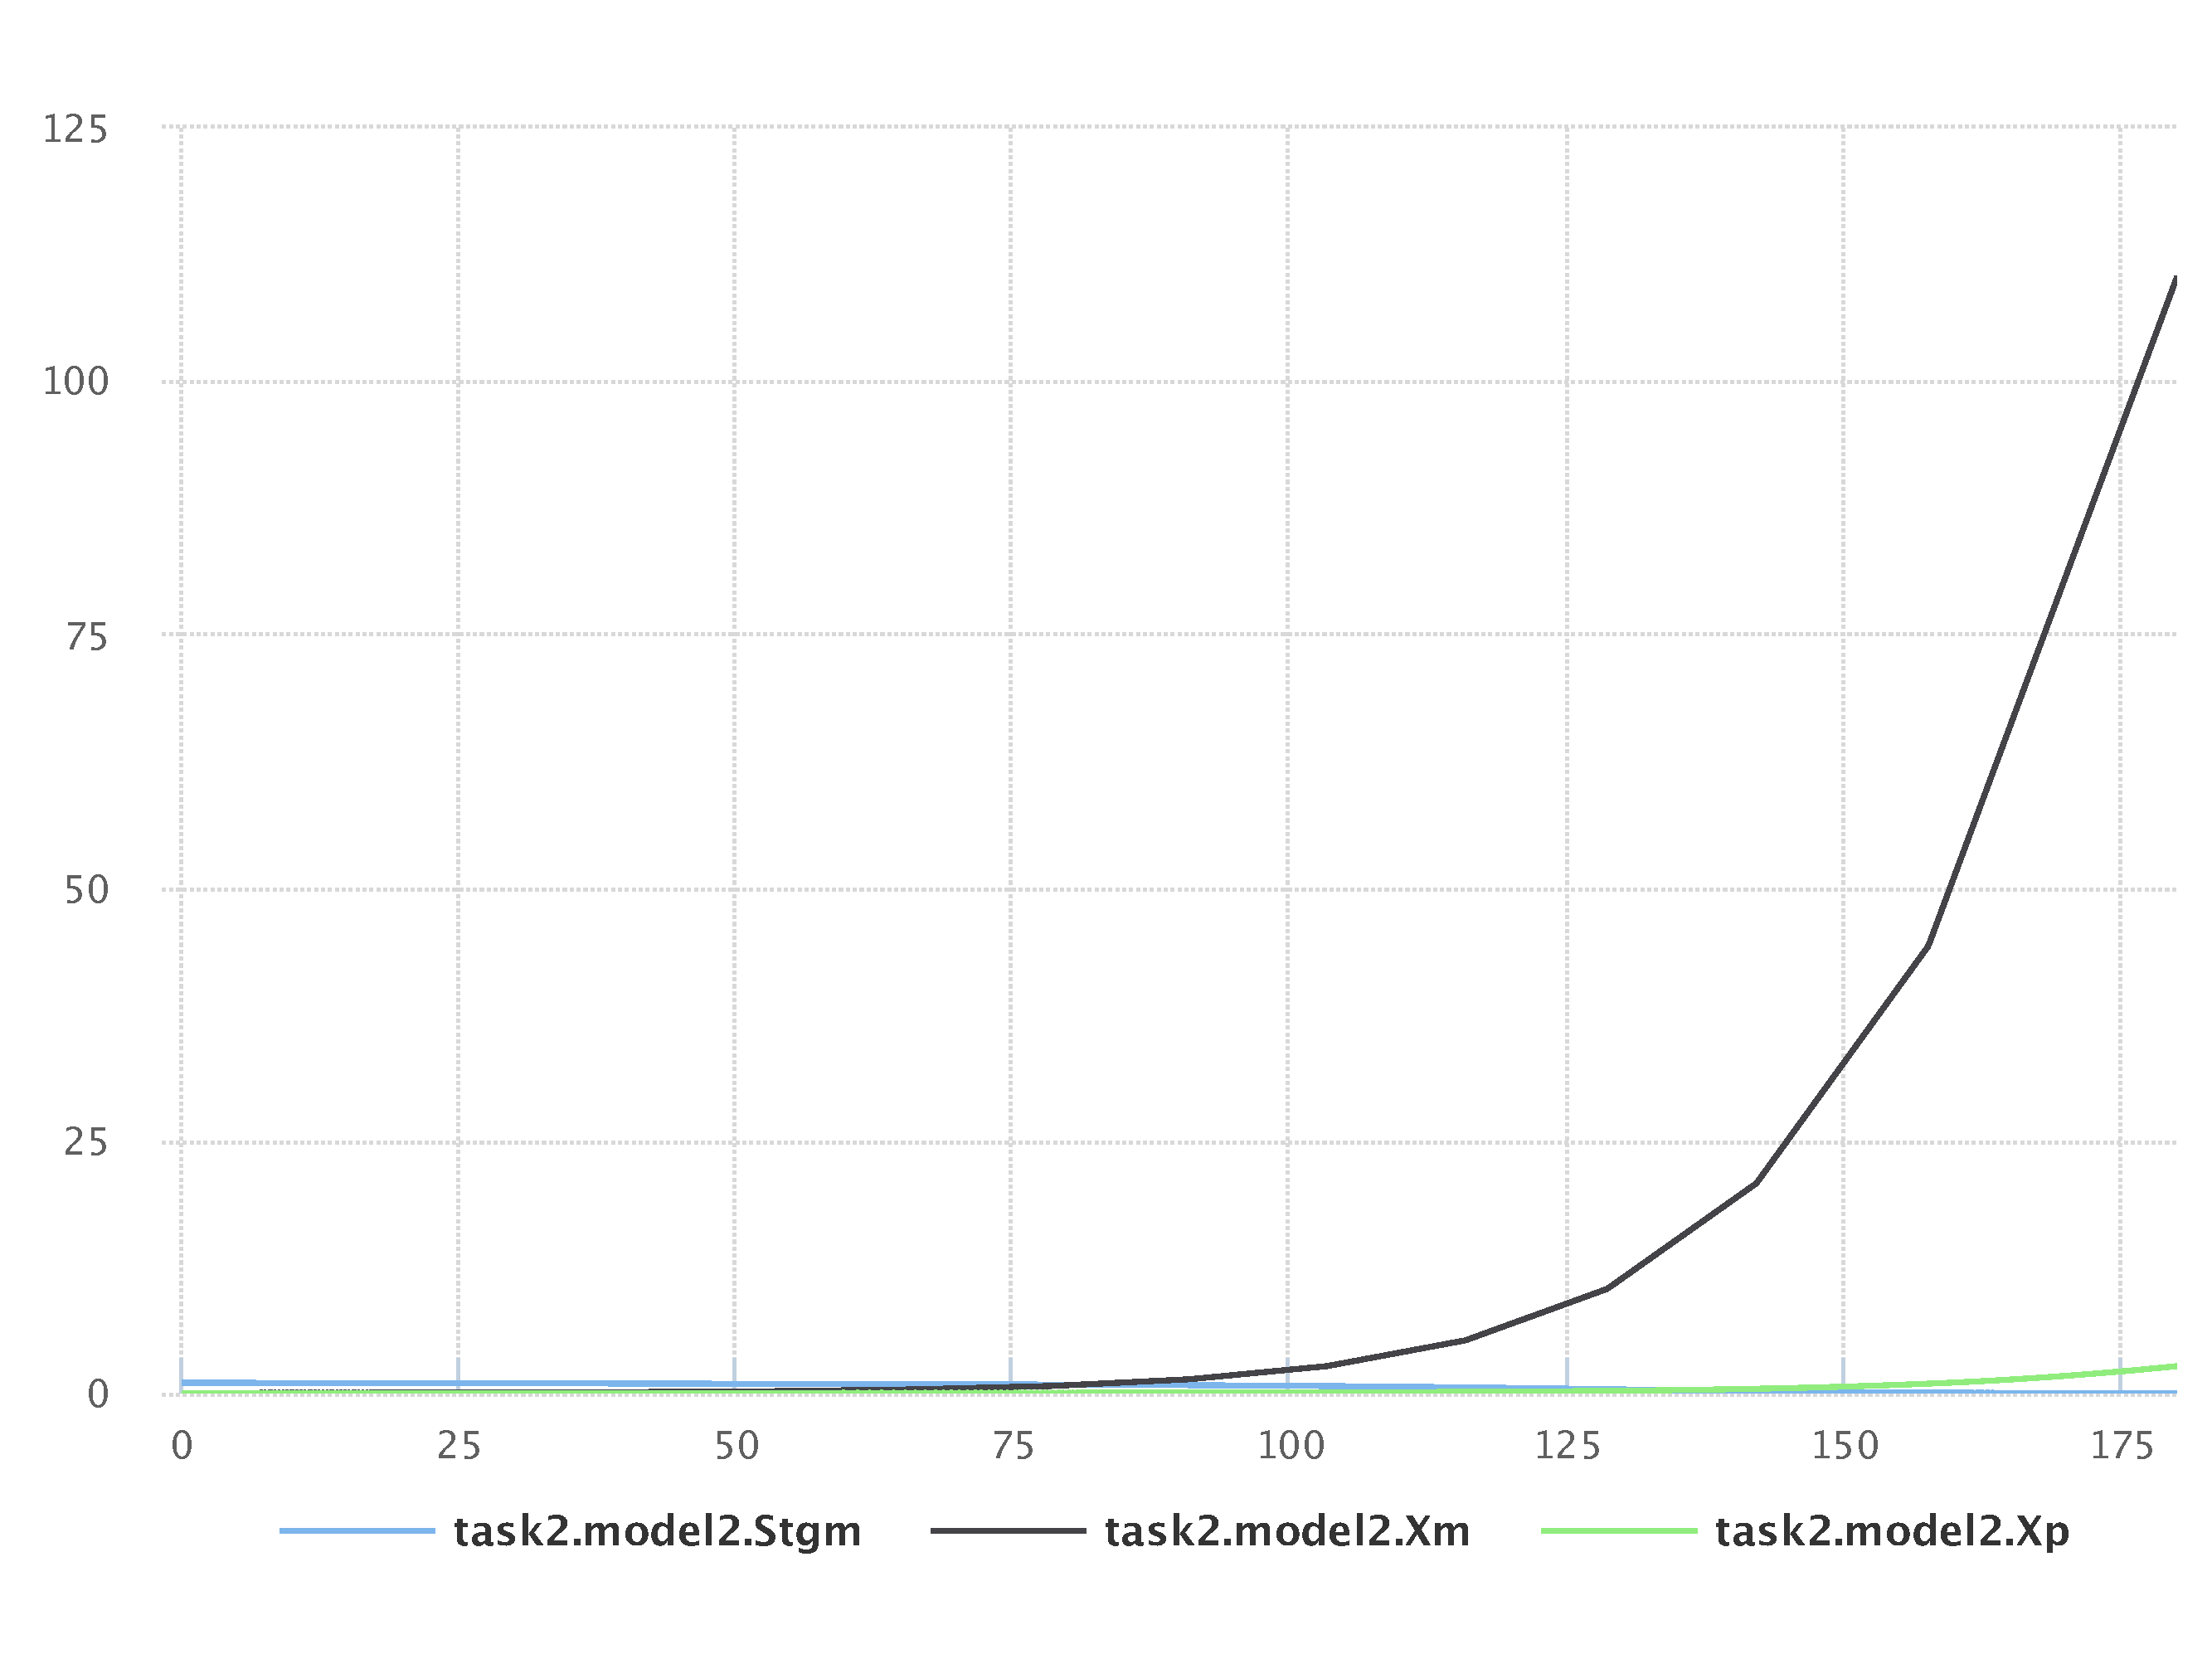
\includegraphics[width=0.75\textwidth]{swt-calzone6.pdf}
  \end{subfigure}
  \caption{ Demonstrating exchangeability of the second case study. To show that the extended set of simulations from Fig \ref{fig:calzone} can be exchanged with other tools via a COMBINE archive, we exported the study in Fig \ref{fig:calzone} to the SED--ML Web Tools and verified that the plots were identical to Fig \ref{fig:calzone}. }
  \label{fig:swt-calzone}
\end{figure}

\clearpage

\begin{figure}
  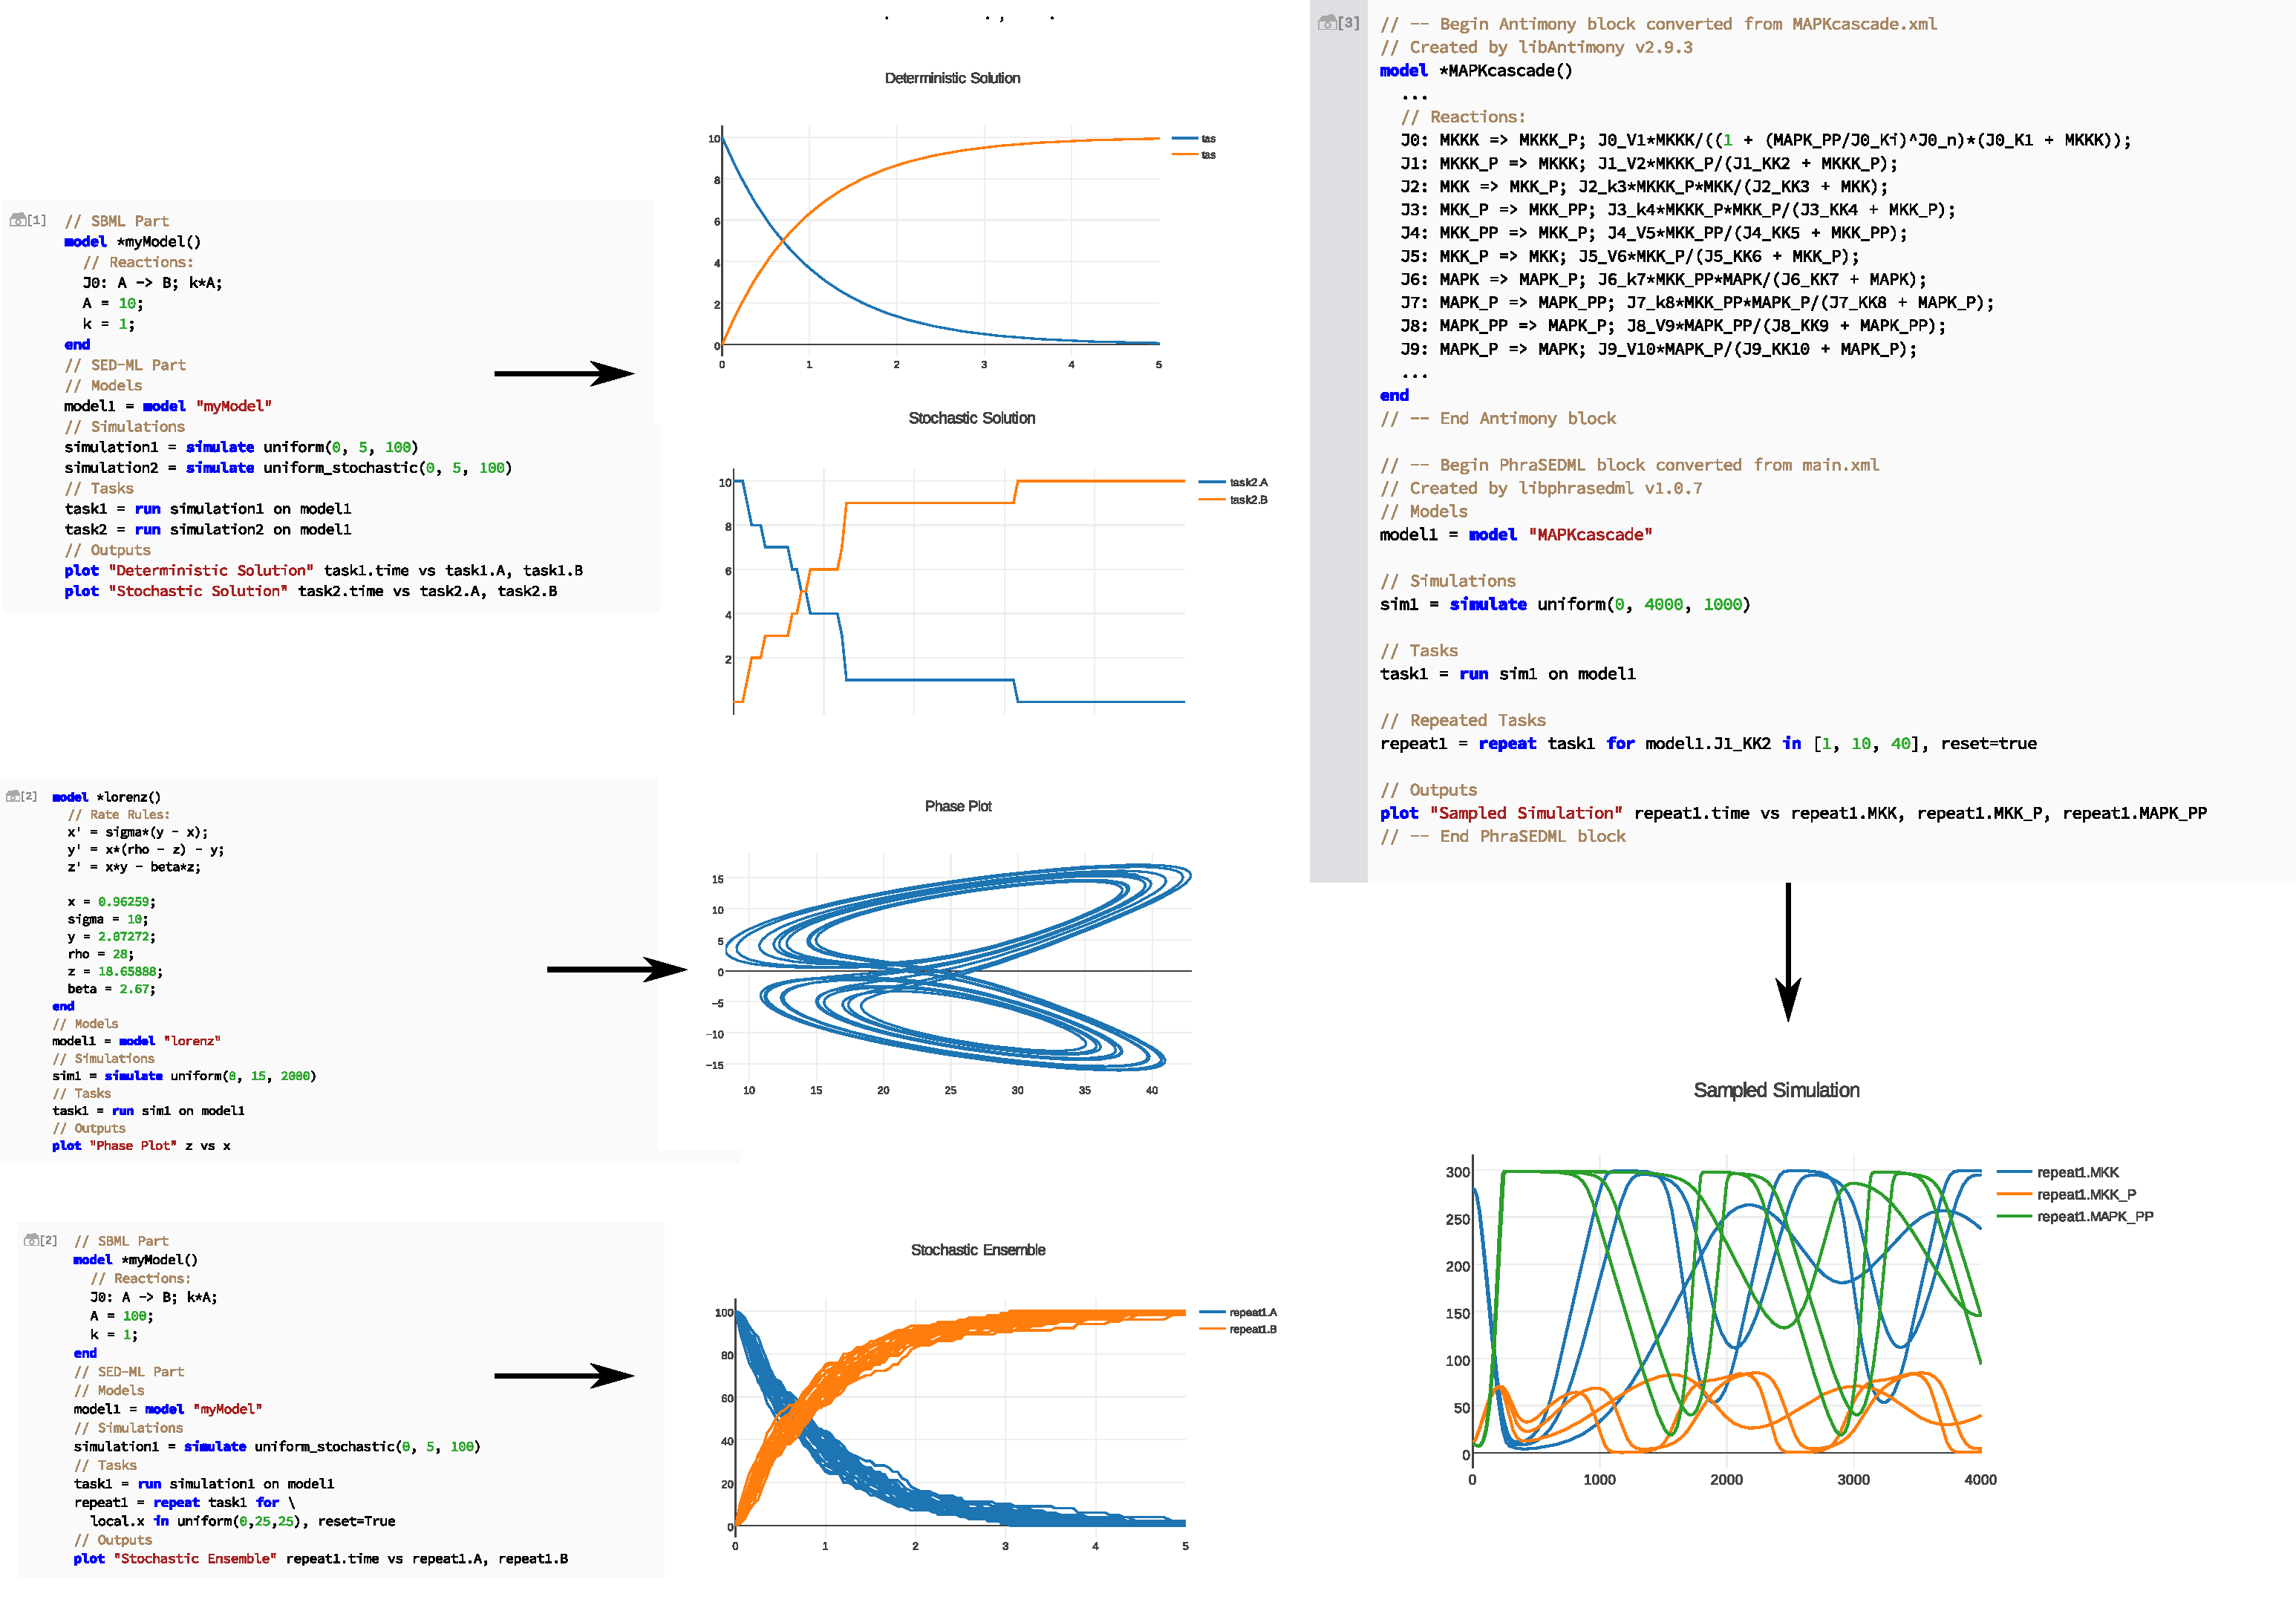
\includegraphics[width=1.0\textwidth]{fig-inline-omex.pdf}
  \caption{Examples of Tellurium's inline OMEX format for specifying COMBINE archives. These examples start with very simple cases and build on these cases with progressively more advanced features. The first example contains a simple two--species model and simulated using a deterministic and stochastic solver. The second example shows a phase plot. The third example shows multiple stochastic traces. The fourth example shows a one--dimensional parameter scan. All of these examples are available via a Tellurium notebook, which can be accessed by clicking on ``File'' $\rightarrow$ ``Open Example Notebook'' $\rightarrow$ ``COMBINE Archive Basics'' from within the Tellurium notebook viewer. }
  \label{fig:inlineomex}
\end{figure}

\clearpage

\begin{figure}
  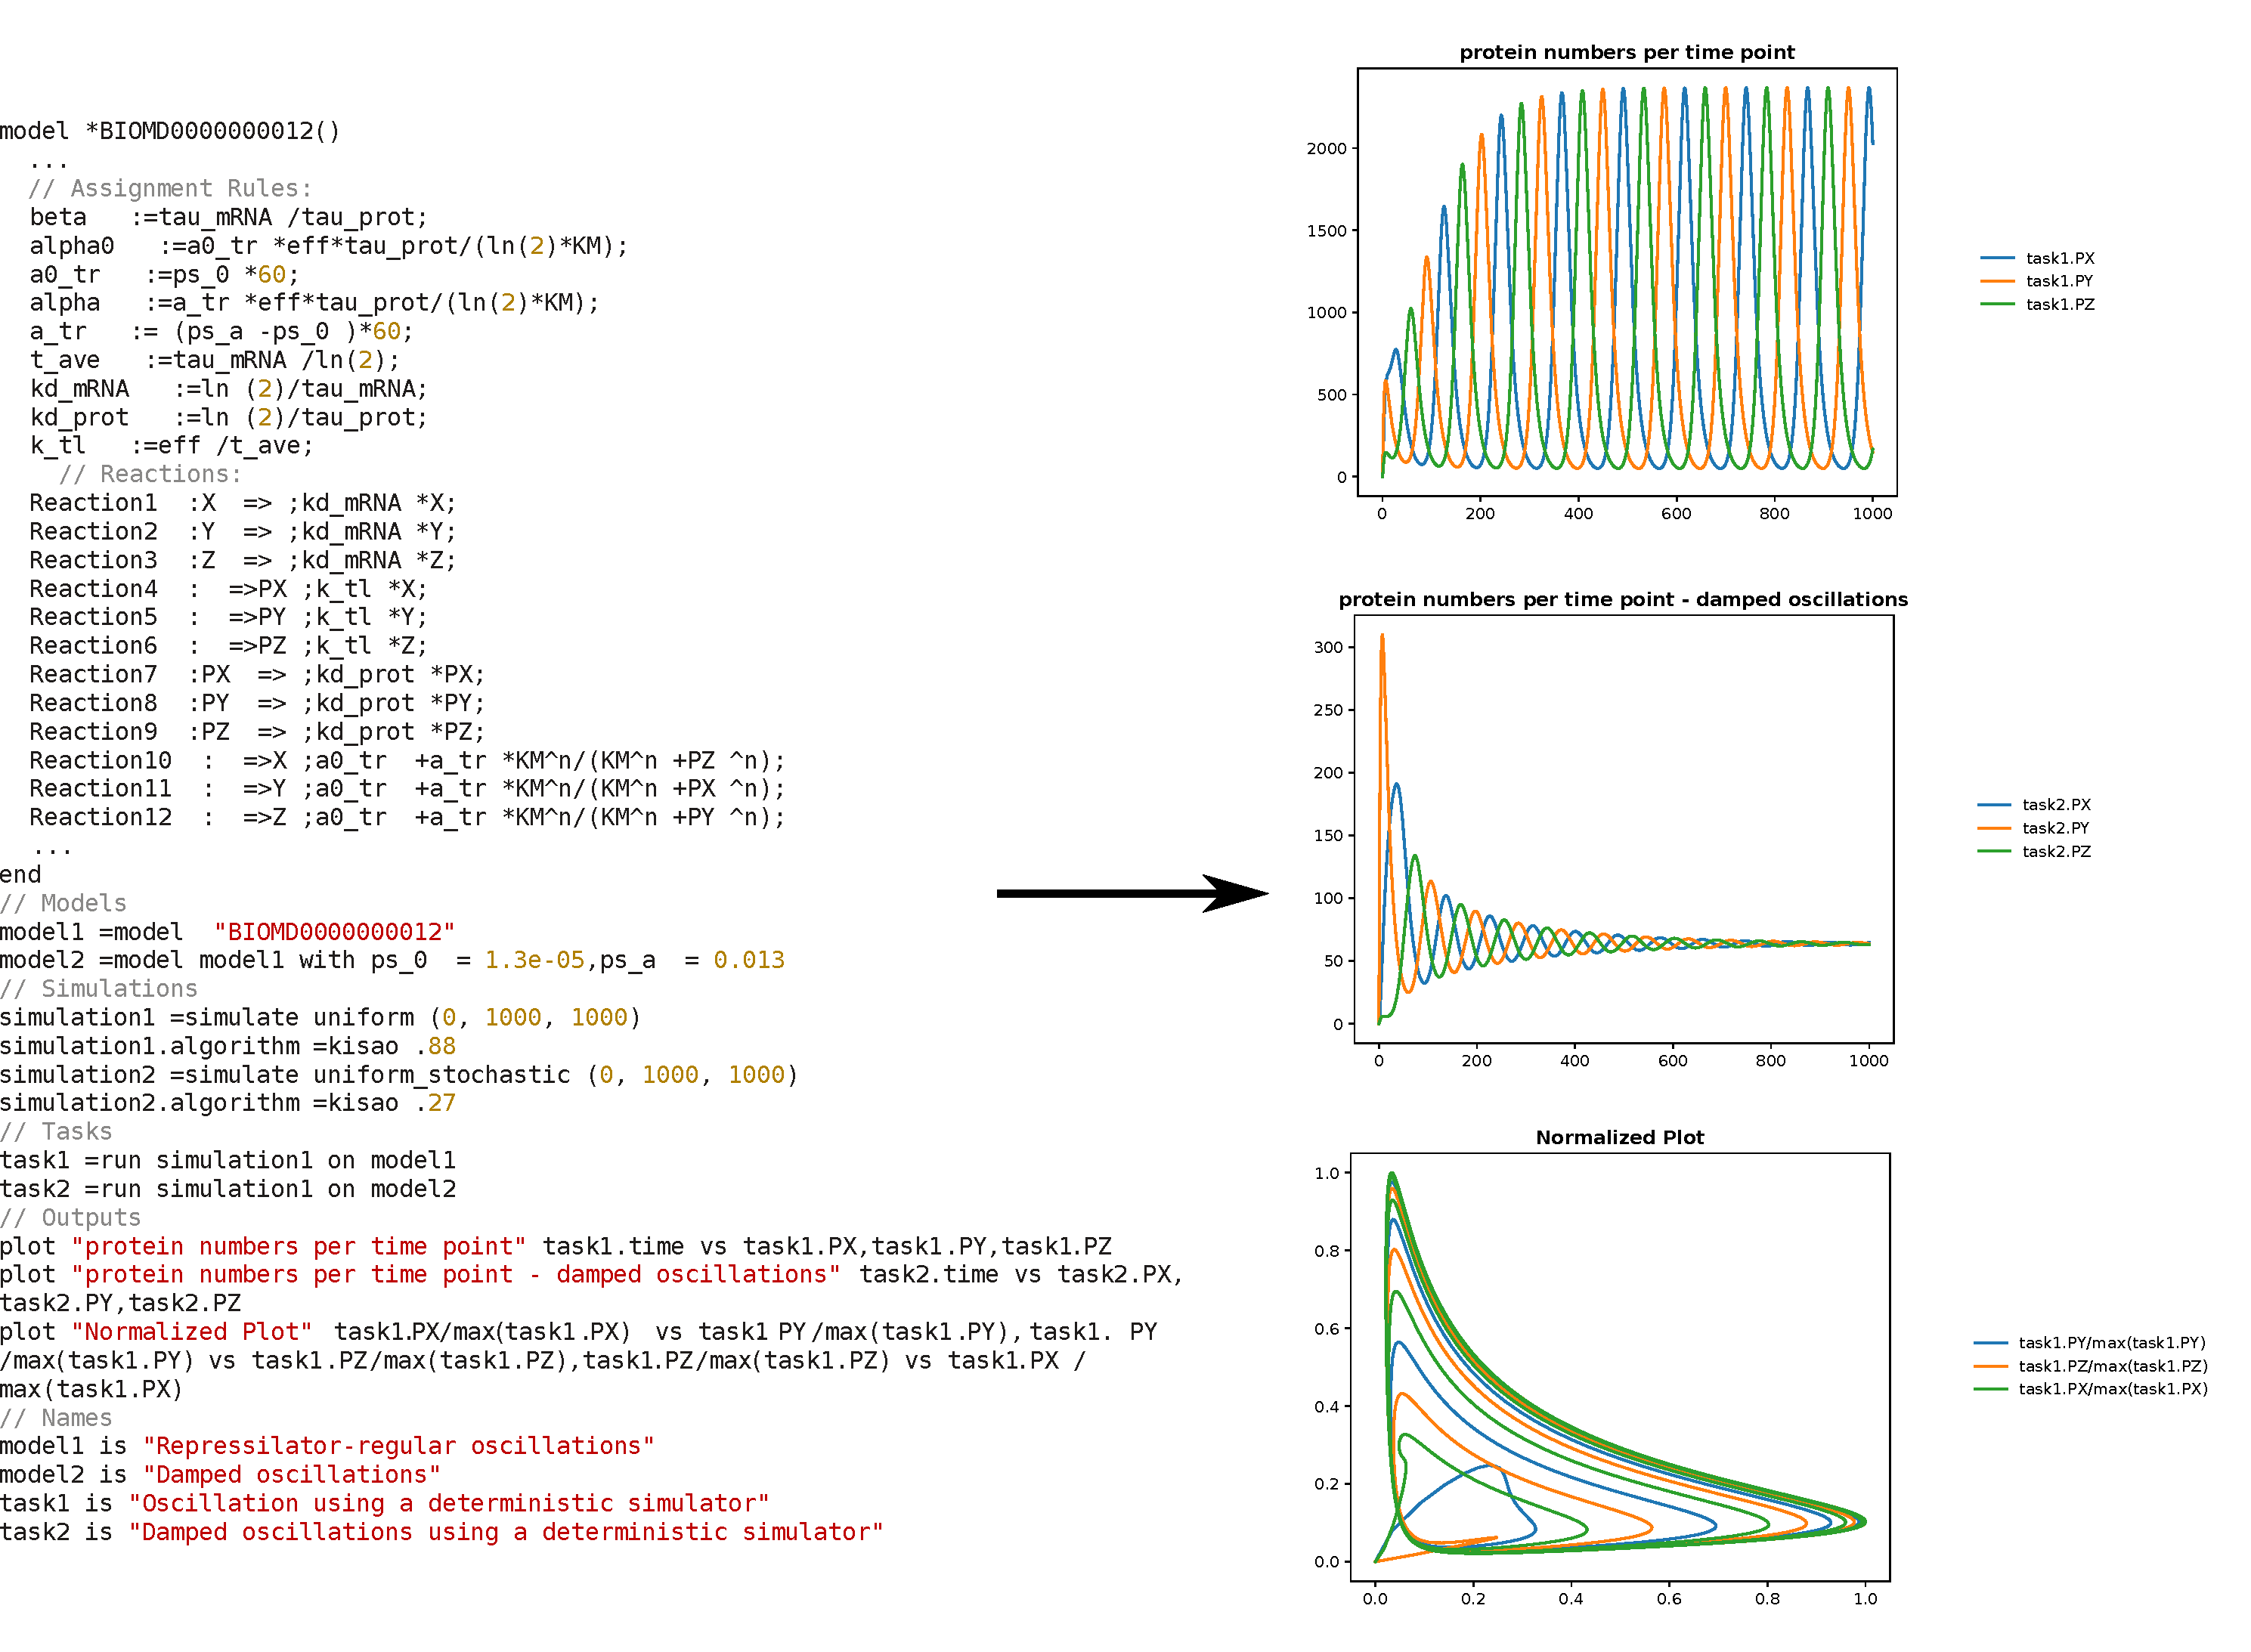
\includegraphics[width=\textwidth]{fig-bergmann2014.pdf}
  \caption{ A normative example of a COMBINE archive introduced  in the original paper describing the COMBINE archive format \cite{bergmann2014combine}. This example contains the repressilator model \cite{elowitz2000synthetic}, a damped oscillation variant showing the modification of model parameters using SED--ML, and a phase plot of the undamped system. }
  \label{fig:bergmann2014}
\end{figure}

\clearpage

% Place tables after the first paragraph in which they are cited.
\begin{table}[t]
%\begin{adjustwidth}{-2.25in}{0in} % Comment out/remove adjustwidth environment if table fits in text column.
\centering
\caption{
{\bf Combine Archive Test Cases.} }
\begin{tabular}{p{12cm}}
\hline %\thickhline
  \texttt{demos}: A set of models and SED--ML simulations of increasing complexity, in order to facilitate incremental support of the standard (4 archives, shown in Fig \ref{fig:inlineomex}). \\ \hline
  \texttt{real-models}: A selection of BioModels converted to COMBINE archives containing the associated SED--ML simulations (2 archives). \\ \hline
  \texttt{published}: COMBINE archives published in the literature, including normative examples from the original paper introducing COMBINE archives \cite{bergmann2014combine} shown in Fig \ref{fig:bergmann2014} (2 archives). \\ \hline
  \texttt{swt}: Examples from the SED--ML Web Tools \cite{bergmann2017sed} demonstrating advanced features of SED--ML (5 archives). \\ \hline
  \texttt{sbml-test-suite}: COMBINE archive encodings of the entire SBML test suite (1196 archives). \\ \hline
\end{tabular}
\begin{flushleft} We collected all COMBINE archives used during development of Tellurium in an online repository on GitHub \cite{catests}. These archives serve to test Tellurium's standards compliance, but they may also allow other tool developers to better support COMBINE archives. We have therefore organized the test cases into different categories, from toy examples using progressively more advanced features of SED--ML, to BioModels, and finally advanced SED--ML usage. The test suite draws archives from a wide range of sources: publications \cite{bergmann2014combine,scharmf1000}, other tools (e.g. the SED--ML Web Tools \cite{bergmann2017sed}), the SBML Test Suite encoded as COMBINE archives, and archives developed by our group. The COMBINE test suite contains archives ranging from basic examples to advanced usage of the SED--ML standard. To verify exchangeability, we have manually tested importing these archives into our software and also into the SED--ML Web Tools. The SBML test cases were too numerous to test in this way, so a subset of archives were tested with the SED--ML Web Tools whereas the full set of archives was tested with Tellurium using a Tellurium notebook \cite{sbmltsnotebook}.
\end{flushleft}
\label{combine-archive-tests}
%\end{adjustwidth}
\end{table}

\clearpage

% Place tables after the first paragraph in which they are cited.
\begin{table}[t]
%\begin{adjustwidth}{-2.25in}{0in} % Comment out/remove adjustwidth environment if table fits in text column.
\centering
\caption{
{\bf Advanced SED--ML Tests (Provided by SED--ML Web Tools \cite{bergmann2017sed}).} }
\begin{tabular}{p{12cm}}
\hline %\thickhline
  \texttt{repeated\_stochastic\_traces.omex}: Repeated runs of a stochastic simulation, overlaying the results of each run. \\ \hline
  \texttt{repeated\_stochastic\_traces.omex}: Scanning the steady state of a model as a function of a parameter. \\ \hline
  \texttt{pulse\_experiment.omex}: Representing a generalized, time--varying forcing function in SED--ML. \\ \hline
  \texttt{pulse\_experiment.omex}: Generalized, time--varying forcing function in SED--ML. \\ \hline
  \texttt{timecourse\_scan.omex}: Timecourse plot of different parameterizations of a model. \\ \hline
  \texttt{nested\_scan.omex}: Nested steady state scan, iterating over two parameters. \\ \hline
\end{tabular}
\begin{flushleft} The SBML test suite was converted into COMBINE archives using the provided notebook \href{https://github.com/0u812/tellurium-combine-archive-test-cases/blob/master/sbml-test-suite/convert-to-combine-arch.ipynb}{https://github.com/0u812/tellurium-combine-archive-test-cases/blob/master/sbml-test-suite/convert-to-combine-arch.ipynb}. These SBML test cases are automatiaclly converted into COMBINE archives containing the expected results, which are then converted by Tellurium into inline OMEX and simulated. A ``failed'' test refers to a case where the numeric simulation results diverge from the expected values. An ``unsupported'' test refers to a test that uses features not available in our simulator (libroadrunner) or the inline OMEX strings.
\end{flushleft}
\label{swt-examples}
%\end{adjustwidth}
\end{table}

\clearpage

% \begin{itemize}
% \item An example showing repeated runs of a stochastic simulation, overlaying the results of each run (\texttt{repeated\_stochastic\_traces.omex}).
% \item An example of scanning the steady state of a model as a function of a parameter (\texttt{repeated\_stochastic\_traces.omex}).
% \item An example showing how to represent a generalized, time--varying forcing function in SED--ML (\texttt{pulse\_experiment.omex}).
% \item A timecourse plot of different parameterizations of a model (\texttt{timecourse\_scan.omex}).
% \item A nested steady state scan, iterating over two parameters (\texttt{nested\_scan.omex}).
% \end{itemize}
%
% Fig \ref{fig:swt-roundtrip} shows the result of a round--trip procedure consisting of exporting the test cases from the SED--ML Web Tools as COMBINE archives, importing the archives into Tellurium, editing the archives in Tellurium, and re--exporting the archives to the SED--ML Web Tools. As these cases utilize advanced features, this procedure demonstrates broad compliance with SED--ML. It also demonstrates the utility of COMBINE archives for exchanging models and simulations between tools.

% Place tables after the first paragraph in which they are cited.
\begin{table}[t]
%\begin{adjustwidth}{-2.25in}{0in} % Comment out/remove adjustwidth environment if table fits in text column.
\centering
\caption{
{\bf Tellurium SBML Test Suite Results.} }
\begin{tabular}{l|l|l|l|}
\hline
{\bf Test Range} & {\bf Number Passing} & {\bf Number Failing} & {\bf Unsupported}\\ \hline %\thickhline
  1-100  & \textbf{91} & \textbf{3} & \textbf{ 6} \\ \hline
101-200  & \textbf{90} & \textbf{1} & \textbf{ 9} \\ \hline
201-300  & \textbf{90} & \textbf{1} & \textbf{ 9} \\ \hline
301-400  & \textbf{99} & \textbf{1} & \textbf{ 0} \\ \hline
401-500  & \textbf{97} & \textbf{3} & \textbf{ 0} \\ \hline
501-600  & \textbf{59} & \textbf{3} & \textbf{38} \\ \hline
601-700  & \textbf{77} & \textbf{1} & \textbf{22} \\ \hline
701-800  & \textbf{86} & \textbf{6} & \textbf{ 8} \\ \hline
801-900  & \textbf{41} & \textbf{2} & \textbf{10} \\ \hline
901-1000 & \textbf{41} & \textbf{2} & \textbf{57} \\ \hline
1001-1196& \textbf{ 0} & \textbf{0} & \textbf{95} \\ \hline
\textbf{Totals}& \textbf{816} & \textbf{25} & \textbf{254} \\ \hline
\end{tabular}
\begin{flushleft} The SBML test suite was converted into COMBINE archives using the provided notebook \href{https://github.com/0u812/tellurium-combine-archive-test-cases/blob/master/sbml-test-suite/convert-to-combine-arch.ipynb}{https://github.com/0u812/tellurium-combine-archive-test-cases/blob/master/sbml-test-suite/convert-to-combine-arch.ipynb}. These SBML test cases are automatiaclly converted into COMBINE archives containing the expected results, which are then converted by Tellurium into inline OMEX and simulated. A ``failed'' test refers to a case where the numeric simulation results diverge from the expected values. An ``unsupported'' test refers to a test that uses features not available in our simulator (libroadrunner) or the inline OMEX strings.
\end{flushleft}
\label{sbmlbenchmark}
%\end{adjustwidth}
\end{table}

\clearpage

\begin{figure}
  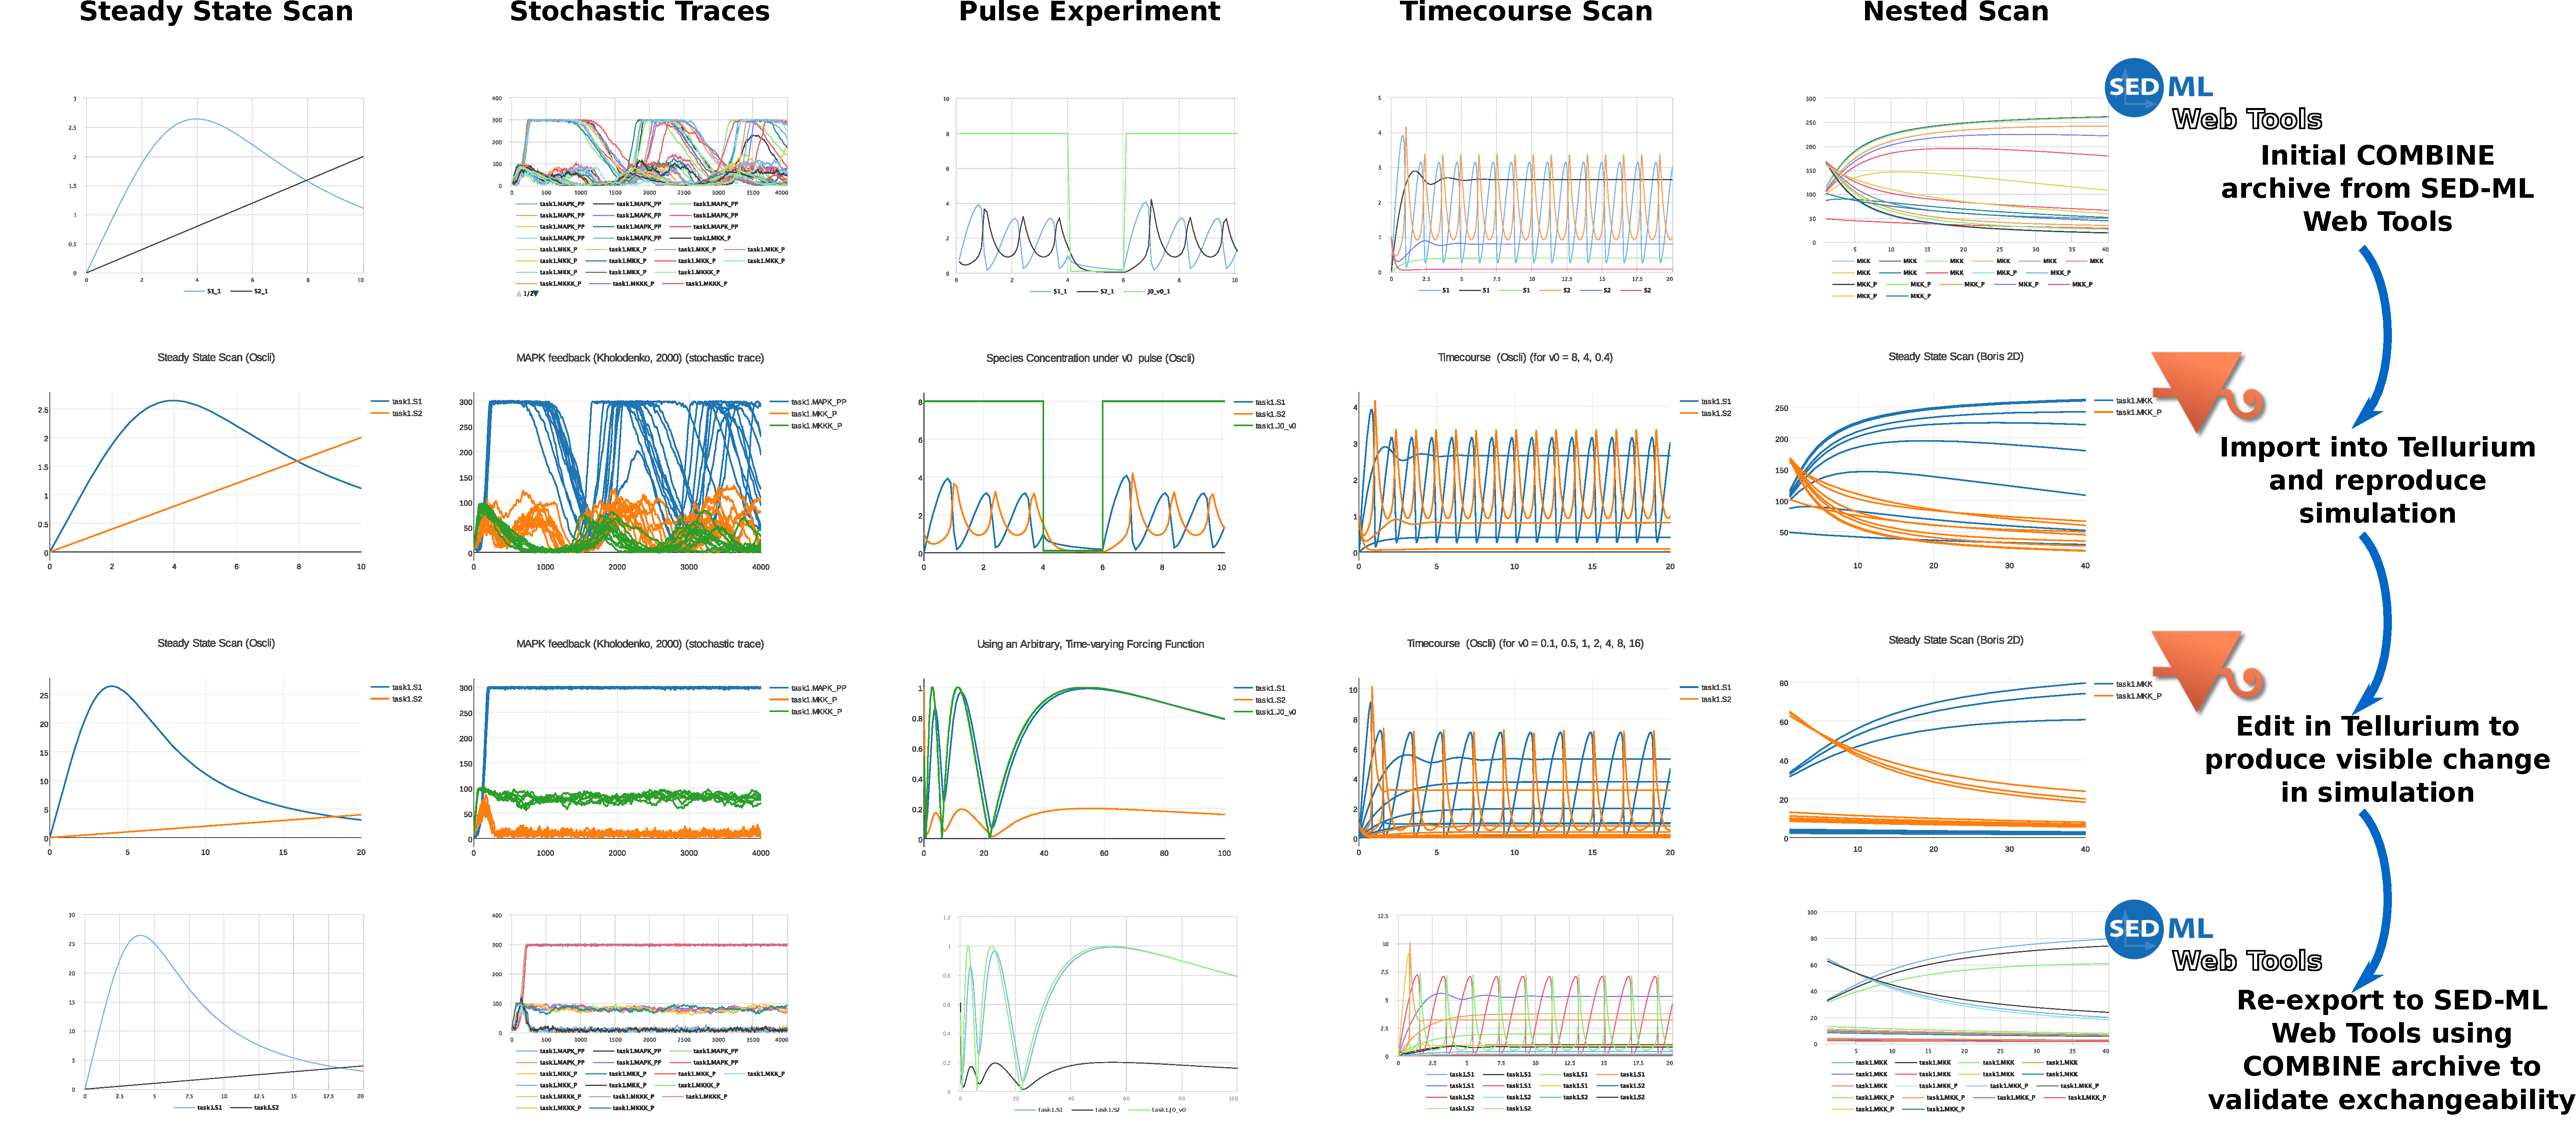
\includegraphics[width=\textwidth]{swt-roundtrip.pdf}
  \caption{Round-tripping the SED--ML Web Tools examples \cite{bergmann2017sed}. In order to demonstrate broad support for standards, we conducted a series of tests utilizing advanced usage of SED--ML. The first row shows the original example rendered in the SED--ML Web Tools. The second row shows the same example imported into Tellurium. The third row shows the simulation after editing the model in Tellurium. Finally, the fourth row shows the result of re--exporting the example to the SED--ML Web Tools using a COMBINE archive. }
  \label{fig:swt-roundtrip}
\end{figure}

\clearpage

% Include only the SI item label in the paragraph heading. Use the \nameref{label} command to cite SI items in the text.

% \paragraph*{S1 Fig.}
% \label{S1_Fig}
% {\bf Bold the title sentence.} Add descriptive text after the title of the item (optional).

% \paragraph*{S2 Fig.}
% \label{S2_Fig}
% {\bf Lorem ipsum.} Maecenas convallis mauris sit amet sem ultrices gravida. Etiam eget sapien nibh. Sed ac ipsum eget enim egestas ullamcorper nec euismod ligula. Curabitur fringilla pulvinar lectus consectetur pellentesque.

% \paragraph*{S1 File.}
% \label{S1_File}
% {\bf Lorem ipsum.}  Maecenas convallis mauris sit amet sem ultrices gravida. Etiam eget sapien nibh. Sed ac ipsum eget enim egestas ullamcorper nec euismod ligula. Curabitur fringilla pulvinar lectus consectetur pellentesque.

% \paragraph*{S1 Video.}
% \label{S1_Video}
% {\bf Lorem ipsum.}  Maecenas convallis mauris sit amet sem ultrices gravida. Etiam eget sapien nibh. Sed ac ipsum eget enim egestas ullamcorper nec euismod ligula. Curabitur fringilla pulvinar lectus consectetur pellentesque.

% \paragraph*{S1 Appendix.}
% \label{S1_Appendix}
% {\bf Lorem ipsum.} Maecenas convallis mauris sit amet sem ultrices gravida. Etiam eget sapien nibh. Sed ac ipsum eget enim egestas ullamcorper nec euismod ligula. Curabitur fringilla pulvinar lectus consectetur pellentesque.

% \paragraph*{S1 Table.}
% \label{S1_Table}
% {\bf Lorem ipsum.} Maecenas convallis mauris sit amet sem ultrices gravida. Etiam eget sapien nibh. Sed ac ipsum eget enim egestas ullamcorper nec euismod ligula. Curabitur fringilla pulvinar lectus consectetur pellentesque.

% \section*{Acknowledgments}
% Cras egestas velit mauris, eu mollis turpis pellentesque sit amet. Interdum et malesuada fames ac ante ipsum primis in faucibus. Nam id pretium nisi. Sed ac quam id nisi malesuada congue. Sed interdum aliquet augue, at pellentesque quam rhoncus vitae.

\clearpage

\nolinenumbers

% Either type in your references using
% \begin{thebibliography}{}
% \bibitem{}
% Text
% \end{thebibliography}
%
% or
%
% Compile your BiBTeX database using our plos2015.bst
% style file and paste the contents of your .bbl file
% here. See http://journals.plos.org/plosone/s/latex for
% step-by-step instructions.
%
\bibliography{main}

%\begin{figure}
%  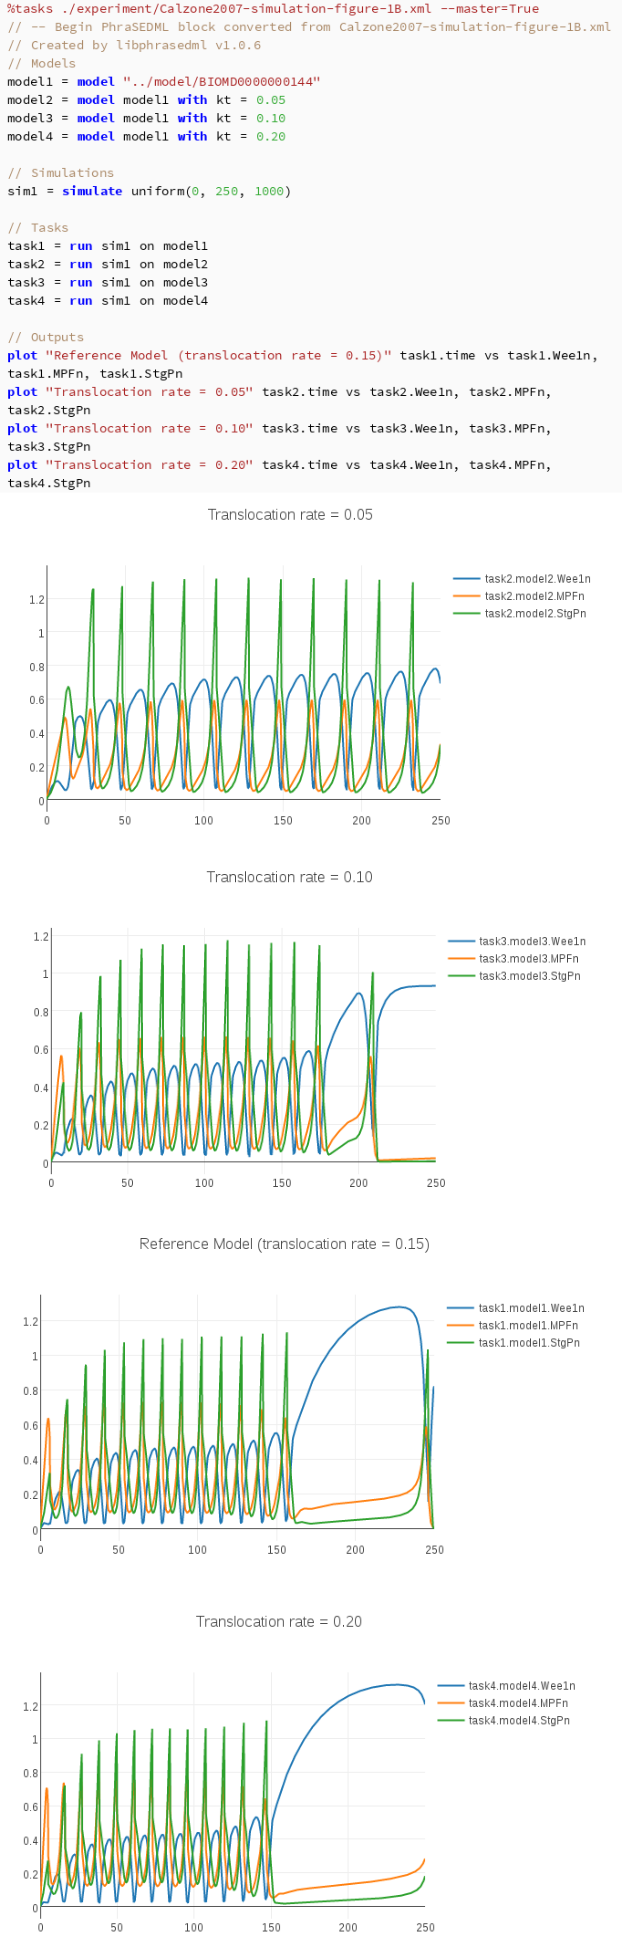
\includegraphics[width=0.5\textwidth]{calzone-tr.png}
%  \caption{Effect of translocation rate on syncytial division dynamics.}
%  \label{fig:calzone-tr}
%\end{figure}

%\begin{figure}
%  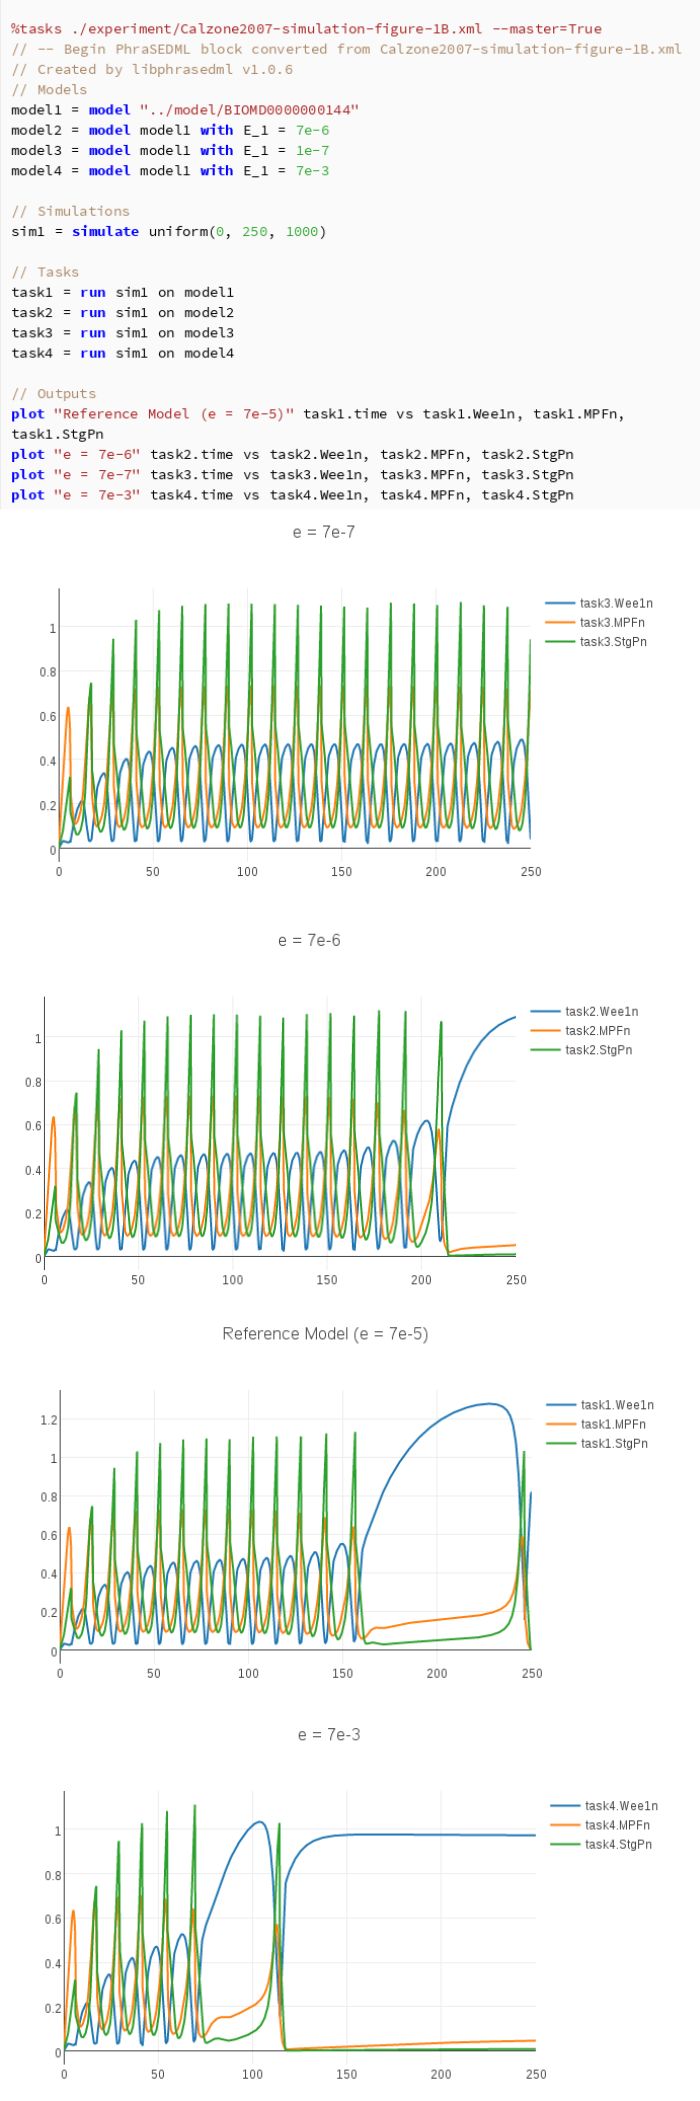
\includegraphics[width=0.5\textwidth]{calzone-e.png}
%  \caption{Effect of nuclear volume fraction on syncytial division dynamics.}
%  \label{fig:calzone-e}
%\end{figure}

%\begin{figure}
%  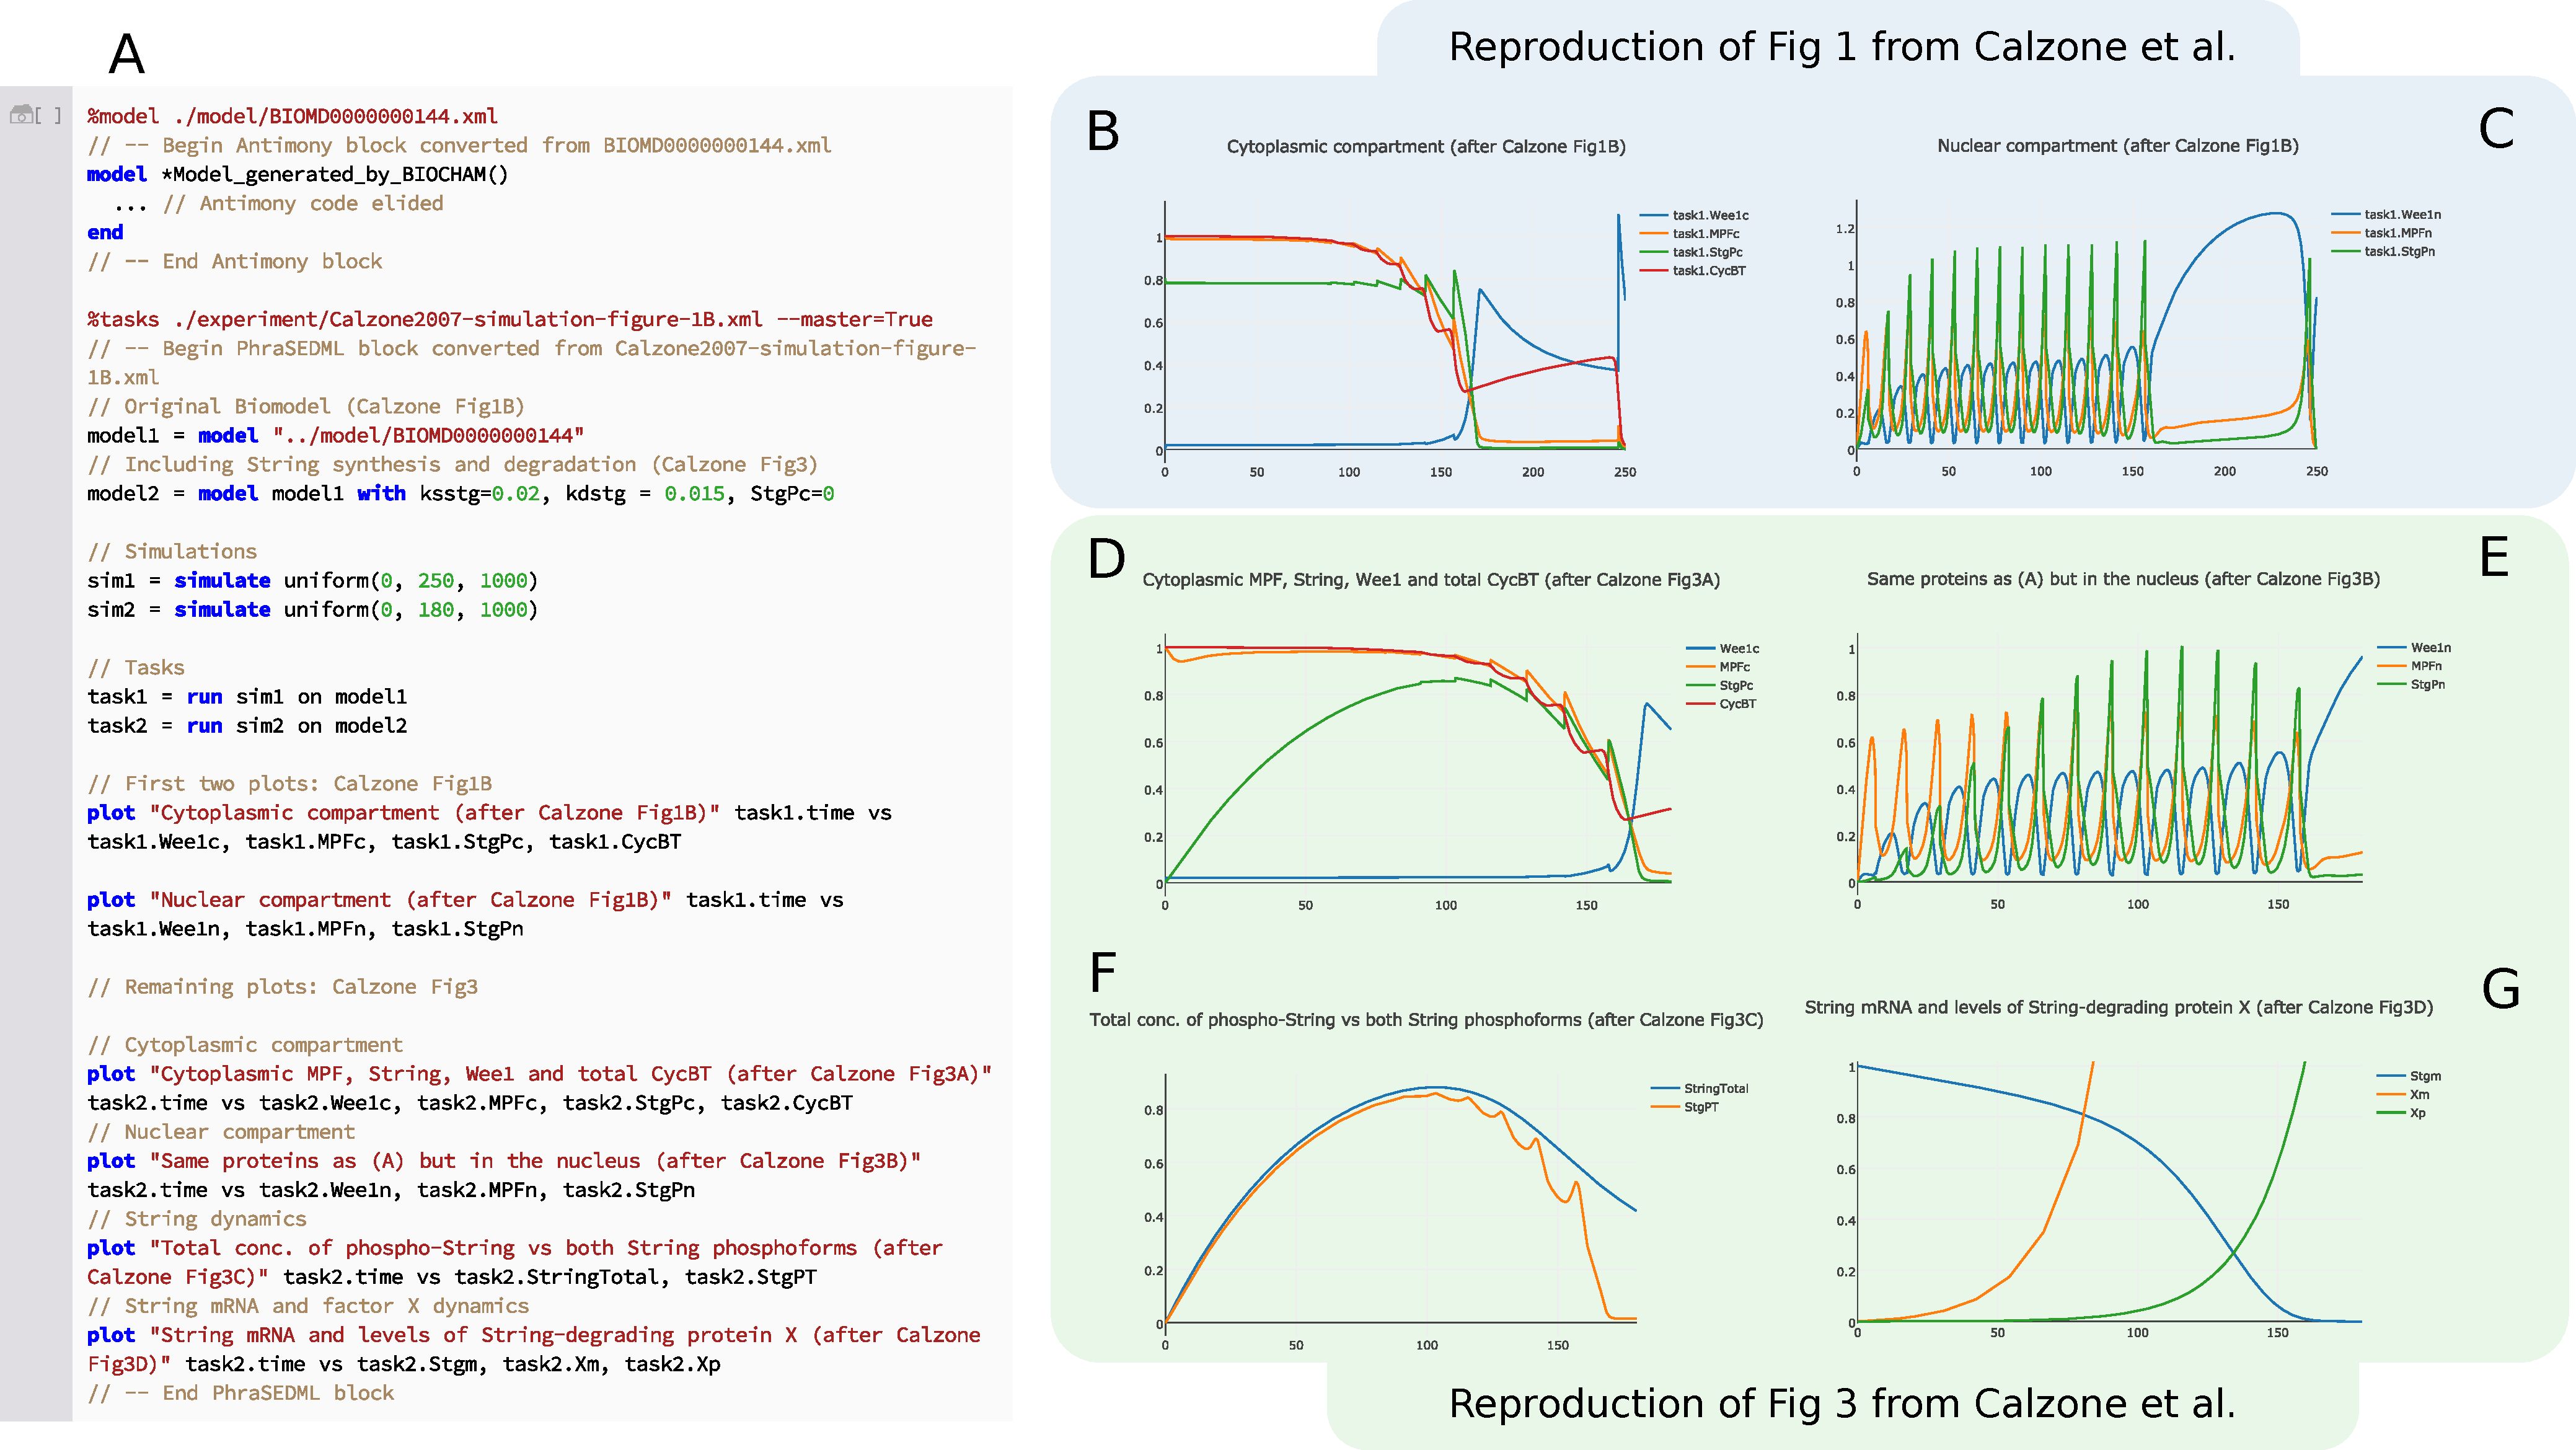
\includegraphics[width=\textwidth]{fig-calzone.pdf}
%  \caption{A COMBINE archive-based reproduction of a model of syncytial mitotic cycles in %\textit{Drosophila} embryos \cite{scharmShowcase,bergmann2017} originally published in \cite{calzone2007dynamical}. Left-hand panels (A and B) represent the cytosol and right-hand panels (C and D) represent the nuclear compartment. This two-compartment scheme was created to model the effects of localization of a key mediator of negative feedback which is localized at centrosomes. The first row (A and C) represent simulations for the two compartments in the original archive. The second row (B and D) represent the effect of changing a single parameter \texttt{factor\_1} from  to . }
%  \label{fig:combineshowcase}
%\end{figure}

\end{document}
